
\errorcontextlines=200

\documentclass[finalspec]{sbmlpkgspec}
%% \documentclass[draftspec]{sbmlpkgspec}
\usepackage{microtype}
\usepackage{color}
\usepackage{todonotes}
\usepackage[color]{changebar}
\usepackage{xcolor}
\usepackage{soul}
\usepackage{subcaption}

% Make changebars switchable to allow faster compilation:
%\def\fullchangebars{} % comment this out to simplify changebars and speed up compilation

% Macros just for this document:

\newcommand{\sbmlpkg}{\texorpdfstring{%
    \textls[-25]{\textsc{SBMLPkgSpec}}}{%
    \textsc{SBMLPkgSpec}}\xspace}
\newcommand{\sbmlpkghead}{\texorpdfstring{%
    \textls[-50]{\textsc{SBMLPkgSpec}}}{%
    \textsc{SBMLPkgSpec}}\xspace}
\newcommand{\sbmlpkgfile}{\literalFont{sbmlpkgspec.cls}\xspace}
\newcommand{\latex}{\LaTeX{}\xspace}
\newcommand{\tex}{\TeX{}\xspace}
\newcommand{\distURL}{http://sourceforge.net/projects/sbml/files/specifications/tex}
\newcommand{\srcURL}{https://sbml.svn.sourceforge.net/svnroot/sbml/trunk/project/tex/sbmlpkgspec}
\newcommand{\webURL}{http://sbml.org/Documents/Specifications/The_SBMLPkgSpec_LaTeX_class}
\newcommand{\cmd}[1]{\literalFont{\textbackslash #1}}

% Custom latex listing style, for use with the listings package.  The default
% highlights far too many things, IMHO.  This keeps it simple and only adjusts
% the appearance of comments within listings.

\lstdefinelanguage{mylatex}{%
  morekeywords={},%
  sensitive,%
  alsoother={0123456789$_},%$
  morecomment=[l]\%%
}[keywords,tex,comments]

\lstdefinestyle{latex}{language=mylatex}


%Command to format the listings containing SBOL RDF/XML serialization examples
\newcommand{\lstsetsbol}{
 \lstset{language=sbol,
        tabsize=2
 }
}

%Commands to format SBOL terms in the document

% Use sbolheading when you are referencing an SBOL data model class/field in a
% section heading.
\newcommand{\sbolheading}[1]{\texttt{#1}}

% Use sbol when you are referencing an SBOL data model class/field in text.
\newcommand{\sbol}[1]{\texttt{\hyperref[sec:#1]{#1}}}

% Use prov when you are using a class borrowed from Prov-O, this will prepend the "prov:" prefix as well
\newcommand{\prov}[1]{\texttt{\hyperref[sec:prov:#1]{prov:#1}}}

% Use provmult for Prov-O fields that appear in multiple classes, for example
% \sbolmult{hadRole:U}{hadRole}. This ensures the reference links to the correct
% section.
\newcommand{\provmult}[2]{\texttt{\hyperref[sec:prov:#1]{prov:#2}}}

% Use om when you are using a class borrowed from Ontology of Units & Measures, this will prepend the "om:" prefix as well
\newcommand{\om}[1]{\texttt{\hyperref[sec:om:#1]{om:#1}}}

% Use provmult for OM fields that appear in multiple classes, for example
% \sbolmult{hadUnit:M}{hadUnit}. This ensures the reference links to the correct
% section.
\newcommand{\ommult}[2]{\texttt{\hyperref[sec:om:#1]{om:#2}}}

% Use sbolmult for SBOL fields that appear in multiple classes, for example
% \sbolmult{types:CD}{types}. This ensures the reference links to the correct
% section.
\newcommand{\sbolmult}[2]{\texttt{\hyperref[sec:#1]{#2}}}

% Rarely used. Use refObj you want to put the field in angle brackets.
\newcommand{\refObj}[1]{$\langle$#1$\rangle$}

%Command to format external terms in the document
\newcommand{\external}[1]{\texttt{#1}}

%Commands to highlight SBOL versions
\newcommand{\threezeroone}[1]{%
	\cbcolor{red}
	\cbstart%
	{\color{red}%
		\version{3.0.1}%
		#1
	}
	\cbend
}

% -----------------------------------------------------------------------------
% Start of document
% -----------------------------------------------------------------------------

\begin{document}

\packageTitle{\latex Class for SBML Package Specifications}		
\packageVersion{Version 3.0.1}		
\packageVersionDate{October 15, 2020}
 
\title{
  Synthetic Biology Open Language \texorpdfstring{\\[3pt]}{}\mbox{(SBOL) Version~3.0.1}}

\author{{\bf Editors:}\hfil\\
\begin{tabular}{l>{\hspace*{15pt}}r}
Hasan Baig & \emph{University of Connecticut, USA}\\   
Pedro Fontanarrosa & \emph{University of Utah, USA}\\   
Vishwesh Kulkarni & \emph{University of Warwick, UK}\\ 
James McLaughlin & \emph{Newcastle University, UK}\\
Prashant Vaidyanathan & \emph{Microsoft Research, UK}\\ 
\multicolumn{2}{c}{\href{mailto:editors@sbolstandard.org}{\sffamily editors@sbolstandard.org}}\\
\\
\multicolumn{2}{c}{ {\bf Chair:} } \\
Chris Myers		& \emph{University of Utah, USA}\\
\\
\multicolumn{2}{c}{{\bf Additional authors:}} \\
Bryan Bartley & \emph{Raytheon BBN, USA} \\
Jacob Beal & \emph{Raytheon BBN Technologies, USA}\\ 
Matthew Crowther & \emph{Newcastle University, UK} \\
Thomas Gorochowski & \emph{University of Bristol, UK}\\
Raik Gr\"unberg & \emph{KAUST, SA}\\
Goksel Misirli & \emph{Keele University, UK}\\ 
Ernst Oberortner & \emph{DOE Joint Genome Institute, USA}\\
James Scott-Brown & \emph{University of Oxford, UK} \\
Anil Wipat & \emph{Newcastle University, UK}\\
\end{tabular}\\
}

\maketitlepage

\maketableofcontents

% -----------------------------------------------------------------------------
\section{Purpose}
% -----------------------------------------------------------------------------
% Synthetic biology aims to apply engineering principles such as standardization, modularity, and design abstraction to molecular biology.  However, synthetic biology still faces substantial challenges, including long development times, high rates of failure, and poor reproducibility. 

% The Synthetic Biology Open Language is intended to help synthetic biologists collaborate by allowing them to exchange designs in a standardized data format.  In addition, the SBOL data model systematically describes the essential details of a design that are required for researchers to reproduce each other's designs in the laboratory.  The purpose of the Synthetic Biology Open Language is to aid collaboration between researchers, improve scientific reproducibility, and to speed the research and development of technologies based on synthetic biology.

% Below is my revision. Any thoughts? - Nic

Synthetic biology builds upon the techniques and successes of genetics, molecular biology and metabolic engineering by applying engineering principles to the design of biological systems. These principles include standardization, modularity, and design abstraction. The field still faces substantial challenges, including long development times, high rates of failure, and poor reproducibility. One of the greatest challenges is the exchange of information between laboraties. Synthetic biology typically relies upon associating a given sequence with a functional role. Often the functional role may be associated with another type of molecule entirely, such as a small chemical, a DNA, an RNA or a Protein molecule. An example is an DNA sequence that is transcribed into a messenger RNA that contains an encoded microRNA binding site, and the messenger RNA in turn being translated into a protein molecule which is a transcription factor binding protein. Functionally the representation of the products of the DNA sequence need to describe the role of microRNA binding to the messenger RNA leading to possible  degredation, or the functional consequence of the protein being absent, leading to repression of expression of another gene. The DNA sequence itself is one or two steps removed from the functional role of the designed device or circuit. Current file formats such as Genbank and SwissProt represent sequence information based upon annotation of sequence features - they do not represent the functional consequence of these sequences. Systems Biology Markup Language represents reactions, pathways and models but does not typically represent the associated sequences. Synthetic biology needs a standard with common formats to represent relevant molecues and their functional roles within the designed system, standarized rules on how such information is encoded in the file and the means to enable exchange of such data between participating laboraties as part of publications. 
\Ctodo{Maybe discuss more about how SBOL is a standard. Huge transition from what is Syntetic Biology to SBOL}
\Rtodo{Added some text on the need for a standard and why other standards do not meet the current needs for SynBio data exchange - KC}


To help address these challenges, the Synthetic Biology Open Language (SBOL)Standard introduces a standardized format for the electronic exchange of information describing the structural and functional aspects of biological designs. The standard is designed to support the development of explicit and unambiguous data models of biological designs through the use of a well defined format on how to represent the component molecues, and theri structural and functional roles in a systematic fashion. The stanrard describes rules and best practices on how to include, develop and populate this format with relevant information of essential design details. Because the standard itself can represent information from other sources for sequence representations, reaction information and ontologies to represent biological design information, the standard uses modern information exchange techniques such as Universal Resource Identifiers (URIs). This permits the reuse of existing information without the need to repeat it, thus avoiding both redundancy and future information rot. The ultimate utility of URIs in the SBOL Standard is the ability to support flexible annotation with meta data while associating an authority with that annotation. The definition of the data model and associated format, the rules on the addition of data within the format and the representation of this in electronic data files make the SBOL Standard an excellent means of promoting global data exchange between laboraties and between software programs.
\Ctodo{it's not about a file format, it's about a representation; the fact that this is a file format is incidental -JSB}

\Ctodo{Motivate/discuss URI's?}
\Ctodo{Explicit and unambiguous data model, promotes global data exhchange, allows flexible annotation with meta data while associating an authority with that annotation.}
\Rtodo{reworked the text to add in the suggestions from the associated comments - KC}


\Ctodo{Should the comparison with 1.1 really be there?  This needs revision to be stand-alone, and right now it's basically an extract of the SBOL2 paper -JSB}
Version 1.1 of the SBOL standard focused on representing the structural aspects of genetic designs. To serve as an effective medium for the computational exchange of genetic designs, SBOL must be extended to capture more aspects of a designed system, including both structural and functional information, and the composition of complex structural and functional designs by combining simpler parts. The SBOL data model proposed in this specification provides for addressing the most pressing needs for expanding SBOL Version 1.1. 

\begin{enumerate}

\item represent structural components of a biological design, including DNA, RNA, proteins, small molecules and other physical components

\item describe behavioral aspects of a biological design, the intended or expected interactions and dynamic behavior

\item associate structure and function together, so that a single design can be understood both in terms of its structure and its behavior

\item support rich annotations of all components, so that data required to describe a design, but not formalized in this specification can be safely exchanged

\end{enumerate}

Taken together, these capabilities allow SBOL sufficient expressivity to support the description and exchange of hierarchical, modular representations of both the intended structure and function of designed biological systems.

To address the need for functional descriptions in SBOL, the proposed data model adds classes for modules, interactions, and models. These classes provide a firm basis for functional representation in SBOL without going so far as to create a new standard for mathematically modeling biology, as there already exist several established languages for doing so, from the Systems Biology Markup Language (SBML)~\cite{SBML} to CellML~\cite{CellML} and even MatLab~\cite{matlab}. Rather, these classes enable users of SBOL to group components that function together, describe the basic qualitative interactions between these components, and document references to standard mathematical models that are external to SBOL and that provide more detailed descriptions of component function. In other words, a module gathers together a set of component instantiations, a set of interactions between these component instantiations, and a set of references to external models that are expected to be consistent with the module's interactions.

\Ctodo{This just sort of stops.  Need a better end. --JSB}
The SBOL standard has been developed in collaboration between both wet bench scientists and ascientific modelers active within the Synthetic Biology community. As with the earlier SBOL v1.1 standard this community has met to discuss, argue and agree upon needs that the SBOL standard should address. This information has been used by developers within our community to design, develop and test a specification of the standard. The specification has been tested by the community through several iterations for the ability to represent a wide range of synthetic biology design projects as well as the ability to share designs between different laboratories. The standard has been used to develop softwares that employ the standard for developing and sharing synthetic design projects. The purpose of the current specification is to share the details of the SBOL standard with a wider community of users and developers so it can be more widely employed through the scientific community.
\Rtodo{I wrote a final paragraph to }

% -----------------------------------------------------------------------------
\section{A Brief History of SBOL}
% -----------------------------------------------------------------------------
%Add yourself if you have helped and aren't on the list

\Rtodo{The text below needs thorough review by the community.  We are certain that there are many errors, including missing people.  Please send input to fix these errors.  Reviewed: JSB}

In early 2006, Microsoft issued a call for proposals in the field of computational synthetic biology. A proposal was submitted from UW with the aim to kickstart an effort to develop exchange standards for designs in the new field of synthetic biology. Along with five other groups, the UW group was successful in securing a modest grant. 
Part of the funds were used to fund the initial standards meeting held in Seattle on April 26-27, 2008. 
The organizers of the initial meeting were Herbert Sauro, Sean Sleight and Deepak Chandran. 
The meeting included talks by Raik Gruenberg,  Kim de Mora from the Jason Kelly lab, John Cumbers,  Christopher Anderson, Mac Cowell, Jason Morrison, Jean Peccoud, Ralph Santos, Andrew Milar, Vincent Rouilly, Mike Hucka, Michael Blinov, Lucian Smith, Sarah Richardson, Guillermo Rodrigo, Jonathan Goler, and last but not least Michal Galdzicki. 
Michal was to go on and lead the development of PoBol, as it was then called. Mike's early efforts were instrumental in making SBOL the success it is today. He organized annual workshops from 2008 to 2011 and kept the idea of developing a standard alive. 
These were held at the Synthetic Biology Data Exchange Working Group meeting at Stanford on July 26, 2009 and Anaheim, CA on June 13, 2010. 
Included at the Anaheim meeting were Chandran, Densmore, Dmytriv, Galdzicki, Ham, Rodriquez, Peccoud, Sauro, and Stan. 
The original SBOL 1.0 was developed at these early meetings through Michal's efforts, together with the small group of other dedicated researchers. 
It was also that the Anaheim meeting that a decision was made to write a letter to Nature Biotechnology highlighting the issue of reproducibility in synthetic biology. This letter was initiated by Jean Peccoud and submitted by participants of the Anaheim meeting. 

An important meeting was held in 2011 at Blacksburg, Virginia on January 7-10, 2011 where new members joined the group resulting in 17 individuals at the meeting. New members included Cesar Rodriguez, Mandy Wilson, Guy-Bart Stan, Chris Myers, and Nicholas Roehner, and the over all pace of development quickened. 

At a meeting in San Diego in June 2011, the SBOL Developers Group was officially established, rules of governance were established, and the first SBOL editors were elected: Mike Galdzicki, Cesar Rodriguez, and Mandy Wilson.  
At this time, Allan Kuchinsky, a research scientist at Agilent, joined the effort, and he was able to obtain some resources to begin development on what was to become libSBOLj.  
Kevin Clancy from LifeTechnologies also joined at this time, as well as Anil Wipat, Matthew Pocock, and Goksel Misirli from Newcastle University, and Jacob Beal, Aaron Adler, and Fusun Yaman Sirin from Raytheon BBN Technologies.  
In October 2011, SBOL 1.0 was officially released.  At our next meeting in Seattle in January 2012, Herbert Sauro was elected the SBOL Chair, and two new editors were added: Matthew Pocock and Ernst Oberortner.  
At this meeting, the first data exchange between software tools using SBOL was conducted when a design was passed from Newcastle University's VirtualParts Repository to Boston University's Eugene tool, and finally to University of Utah's iBioSim tool. 

In March 2012, SBOL 1.1 was released, the version that this document replaces. 
SBOL 1.1 did not change the data model, but provided a number of small adjustments and clarifications to details of its intended use and implementation, particularly around annotation of sequences and their locational relations.
The 8th SBOL workshop was held in November 2012 at Boston University, and the major topic of discussion was the next version of SBOL.  SBOL 1.1 is limited to describing hierarchical DNA sequences.  
Several extensions were discussed at this meeting, such as a means to describe genetic regulation, which later become the \sbol{Interaction} class, and a means to group components, which later became the \sbol{Module} class.  
In April 2013, at the 9th SBOL workshop at Newcastle University, the framework for SBOL 2.0 was agreed upon.  
Nicholas Roehner, Matthew Pocock, and Ernst Oberortner then began work on a draft proposal for SBOL 2.0.  In January 2014 at the 10th SBOL workshop, this draft was discussed and many refinements were debated and approved.  Another important decision at this meeting was that SBOL should begin investigating joining the COMBINE community of standards (\url{www.co.mbine.org}). 

In the Spring and Summer of 2014, several important events occurred.  In April, several SBOL representatives attended Harmony in Manchester UK to discuss joining the COMBINE community, which was approved by both sides shortly thereafter.  In May, Herbert Sauro, John Gennari, and Chris Myers received a grant from the National Science Foundation to support SBOL (this document and the supporting software are due in no small part to this support).  

In June, a description and our initial, multi-institutional demonstration of the use of SBOL 1.1 was published in Nature Biotechnology \cite{galdzicki2014synthetic}. In July, Nicholas Roehner presented a proposal for the next version of SBOL at the SEED Conference in Los Angeles \cite{roehner2014proposed}.  Finally, in August 2014, the SBOL community attended their first COMBINE workshop as members of the COMBINE community.  At this meeting, many of the final details of SBOL 2.0 were discussed, and the data model presented here is essentially the result of this meeting.

At the Harmony meeting in April 2015 in Wittenberg, Germany, the work on this specification began in earnest.  The key contributors at this meeting and the previous one were: Bryan Bartley (University of Washington), Jacob Beal (Raytheon BBN Technologies), Kevin Clancy (ThermoFischer), Bryan Der (MIT), John Gennari (University of Washington), Curtis Madsen (Newcastle University), Goksel Misirli (Newcastle University), Chris J. Myers (University of Utah), Tramy Nguyen (University of Utah), Matthew Pocock (Newcastle University and Turing Ate My Hamster LTD), Jackie Quinn (Google), Nicholas Roehner (Boston University), Herbert M. Sauro (University of Washington), Anil Wipat (Newcastle University), and Zhen Zhang (University of Utah).


% % -----------------------------------------------------------------------------
\section{Overview of SBOL}
% % -----------------------------------------------------------------------------
Synthetic designs need to convey three types of information:
\begin{itemize}
\item The physical molecule, represented by a sequence or a chemical structure
\item The functional role of the element in the design
\item The functional consequence of this element within the overall design or the biological system where it will perform 
\end{itemize}
In broad strokes, SBOL 1.1 describes the first of these, the physical information, whereas SBOL 2.0 extends the description of the design to include functional information. The physical information about a designed genetic circuit includes the order of its constituents and their descriptions. The exact locations of these constituents and their sequences allow genetic circuits to be defined unambiguously, and reused in other designs. However, SBOL 1.1 lacked the ability to describe functional interactions among elements within a design, nor functional descriptions of the overall system.

\Rtodo {next two paragraphs are un-edited text provid by Kevin C. I will try to reduce these, without losing biological relevance.}

As an example consider the cloning and expression cassette of a plasmid such as pUC18. The device has a number of parts, including a region of E.coli operon lac containing CAP protein binding site, promoter Plac, lac repressor binding site and 5’-terminal part of the lacZ gene encoding the N-terminal fragment of beta-galactosidase. This fragment, whose synthesis can be induced by the chemical IPTG, is capable of intra-allelic complementation with a defective form of beta-galactosidase encoded by host. In the presence of IPTG, bacteria synthesize both the device portion and the host specific fragments of the enzyme and form blue colonies on media containing the chemical X-gal. Insertion of DNA into the MCS located within the lacZ gene (codons 6-7 of lacZ are replaced by MCS) inactivates the N-terminal fragment of beta-galactosidase and abolishes alfa-complementation. Bacteria carrying recombinant plasmids therefore give rise to white colonies. This device and its usage is fundamental to how colony selection of recombinant plasmids is carried out in laboratories around the world. Understanding how such a device works and how it might be adapted to new experimental applications is currently passed on through working with fellow scientists or reading articles in papers and books. But there is no systematic way of communicating the integration of sequence with functional design, so users typically have to look in many different places to develop an understanding of this system. 

To  adequately describe the functional design of this device it is necessary to include information on the physical elements of the design, such as the chemicals, proteins encoded both in the device and well as from the cell host, and complexes of these elements with each other. The design then needs to include information on the local interactions of the system such as IPTG complexing with the terameric repressor of the lac operon, or the lac repressor complexing with the lac repressor binding site. Finally the design needs to specify the models of the system such as consequence of the IPTG disrupting the tetrameric repressor ultimately leading to a working color selection system. The proposed standard is designed to permit users to incorporate as much or as little of this information as needed to share the physical structure of the device, the functional roles of each of the participating elements as well as the model of the overall system within the cell.  


Figure 1 shows, at an abstract level, some of the important classes of information in SBOL. Figure 2 extends this view to provide a more detailed view of these classes. 

\Rtodo {...this section (obviously) under construction. Currently working on my view of Figures 1 and 2. - jhg}


Figure 1 illustrates the relationships between the main classes of information encoded by SBOL.  
The physical structure of an element is represented with a \sbol{ComponentDefinition}, often corresponding to a particular \sbol{Sequence} (e.g., DNA, RNA, amino acids), and with its structure further described in terms of the smaller \sbol{Component} instances contained within, and their absolute and relative positions within the component.
Functional relationships are represented with a \sbol{ModuleDefinition}, often also described by some \sbol{Model}, and with its structure further described in terms of the smaller \sbol{Module} instances contained within, as well as particular components (designated \sbol{FunctionalComponent} to indicate their use in defining a module), and their interactions.

\begin{figure}[ht]
\begin{center}
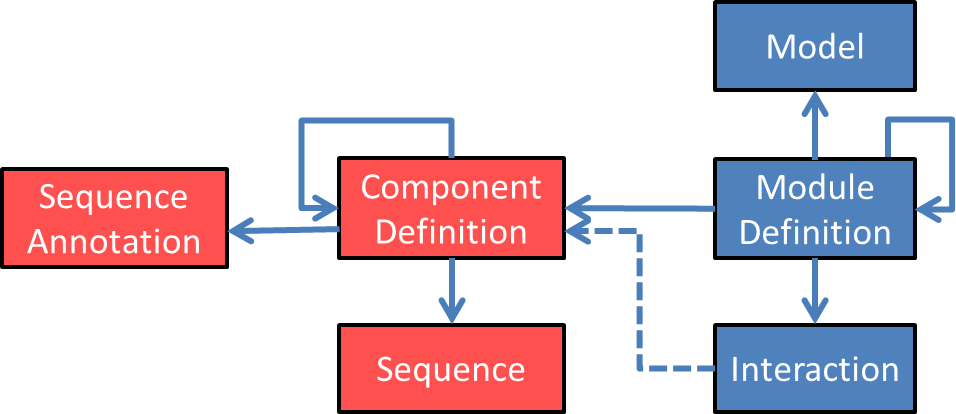
\includegraphics[scale=0.5]{images/OverviewFigforSpec-v3.png}
\caption{Main classes of information represented by the SBOL standard, and their relationships.  Red boxes are classes from the 1.1 version of SBOL that focused on structure, whereas blue classes are some of the new classes that support the functional aspects of designs.}
\label{images:overview1}
\end{center}
\end{figure}

\begin{figure}[ht]
\begin{center}
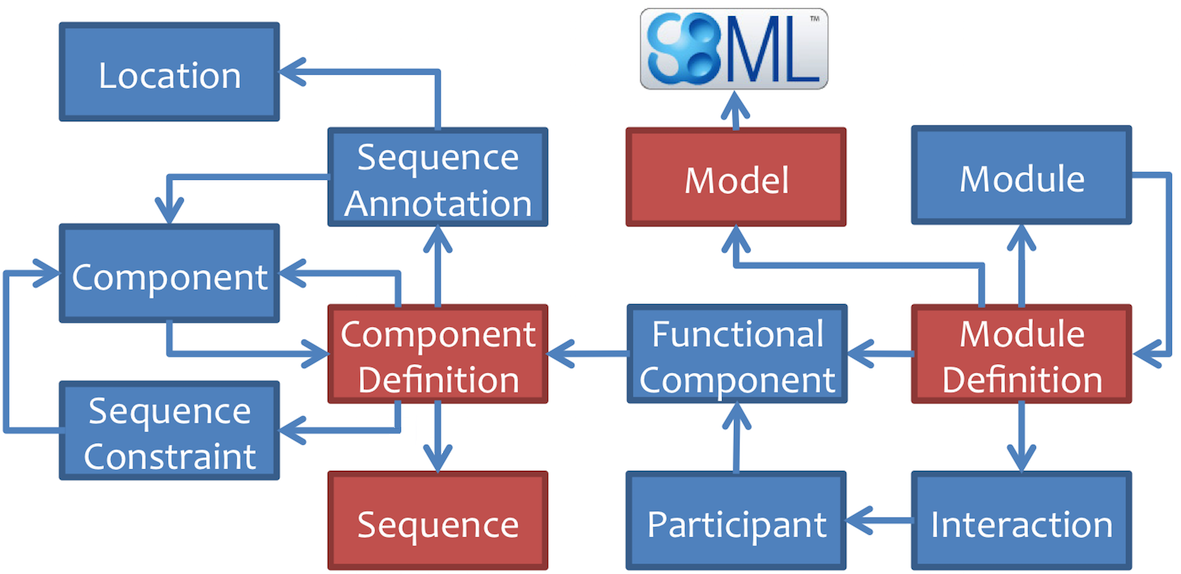
\includegraphics[scale=1.2]{images/SBOL2_2_revised.png}
\caption{Main classes of information represented by the SBOL standard, and their relationships.  Red boxes are ``top level'' classes, while blue classes are used in describing a top-level class; an arrow indicates that one class refers to another.}
\label{images:overview2}
\end{center}
\end{figure}

The \sbol{Sequence} is a fundamental information object for synthetic biology and is needed to reuse components, to replicate synthetic biology work, and to assemble new synthetic biological systems. In designed systems such objects can consist of small chemical molecules, DNAs, RNAs or Proteins. The \sbol{Sequence} object has been designed to encapsulate any of these types of molecules. Small molecule \sbol{Sequence} objects are typically referred to via their chemical formulae. Molecules where sequence specific information is important, such as DNA, RNA and Protein \sbol{Sequence} objects, use the object to incorporate this information. The \sbol{Sequence} object encapsulates this positional information as well as the associated experimental work or other information related to a sequenced molecule.

\Rtodo{need to make it clear that it includes DNA, RNA, and protein, also smooth the text --JSB made addiitons based upon the suggested changes - KC}

In the SBOL data model, a structural layer defines the physical arrangement of components in a biological system.  \sbol{ComponentDefinition}s define genetic elements such as promoters, RBSs, CDSs, and terminators, as well as RNA, proteins, and small molecules.  In a structural hierarchy, \sbol{ComponentDefinition}s can contain subcomponents (\sbol{Component}s), which are instances of the \sbol{ComponentDefinition} for that subcomponent.  A functional layer can be defined to describe the behaviors that arise from the structural layer.  \sbol{ModuleDefinition}s contain information about molecular interactions and their participating components.  They can contain \sbol{FunctionalComponent}s that are instances of \sbol{ComponentDefinition}s that can be assigned functional properties, and they can also contain other modules in a functional hierarchy.  The functions and interactions of these components and other modules within the \sbol{ModuleDefinition} can be quantitatively or qualitatively described using a \sbol{Model}. The \sbol{SequenceAnnotation} object defines data associated the \sbol{Sequence} and \sbol{ComponentDefinition} objects that is needed beyond basic definitions. This can refer to local annotations of the object as well as a container for URIs to external information sources. 


SBOL includes different entities to describe such genetic circuits. Genetic elements such as a promoter, ribosome binding site (RBS), coding sequence (CDS), or terminator are defined with the \sbol{ComponentDefinition} entity. Their instances are reused in different designs via the \sbol{Component}s that refer to corresponding \sbol{ComponentDefinition}s. \sbol{ComponentDefinition}s can also represent proteins, RNAs or small molecules. They are associated with sequence information such as nucleotides aminoacids or chemical structure. A full description of a genetic circuit is then represented using  \sbol{ModuleDefinition}s which contains information about molecular interactions and their participating components. Modules can be associated with quantitative or qualitative models using the \sbol{Model} entity, which is used to point to the actual location of a model. 
\sbol{SequenceAnnotation}s can be used to carry data associated with the successful running of that model on another computer, can be used to point towards sources of some or all of the circuit and the location of experimental data associated with the development of the model.

\Rtodo{Need to also explain annotation --JSB
Provided some text for review describing annotation - KC}



SBOL facilitates the design of complex systems using hierarchical composition. In addition to using simple genetic elements in a modular fashion, modules that are composed of multiple, different components can also be reused. Such modules can expose some of the design components as inputs and outputs, which can be connected to components from other modules using \sbol{MapsTo} entities.


\Ctodo{This needs to be clarified.  Do we really want to explain MapsTo here? -JSB}
\Ctodo{it's not in the diagram. So it should be removed or dealt with in the figure and earlier in the text- KC}

\Ctodo{Explain why it is important to separate definitions from instantiations?}

\LDtodo{The motivation for separating structural and functional considerations is not explained.  Which class names are structural, which class names are functional, and how are the two connected?  Do all structural components require a functional counterpart?  If not, explain why only a subset of structural components would have functional definitions.}

\Ctodo{As a person reading about SBOL2 for the first time, I rank this as the most important section.  While the document should be technically focused overall, this section is your chance to concisely tell someone who won't read the whole document about the take-home messages for the new data model.}

\LDtodo{Why are URI's needed for Components?  Why not just for ComponentDefinitions?  Is there anything in SBOL that does not require a URI?}
\Ctodo{Also briefly mention URI}

\Ctodo{Make sure we explain about annotations up in the motivation and overview, since it's really, really important.}

% The same toggle switch is now displayed using two LacI and TetR inverter submodules in figure \ref{images:toggleswitch_modular}. The LacI inverter uses LacI as input and produces the TetR output, and the TetR inverter uses TetR as input and produces the LacI output. These inputs and outputs are mapped in a parent module.

% Removed as redundant:
%-----------------------------------------------------------------------------
%\section{Introduction}
% -----------------------------------------------------------------------------
%While the first version of the Synthetic Biology Open Language (SBOL) has been adopted by several academic and commercial genetic design automation (GDA) software tools, it only covers a limited range of the requirements for a standardized exchange format for synthetic biology. The SBOL 2.0 specification revises version 1.1, enabling the representation of a wider range of components with and without sequences, including RNA components, protein components, small molecules, and molecular complexes. Additionally, the latest SBOL can be used to convey the intended function of a design, as well as its structural composition. 
%This dichotomous representation of the structural and functional features of a design is a paradigm applied to great success in electrical and computer engineering, and is essential for the development of design automation software in synthetic biology.
%
%The goal of this specification is to define the terminology and relationships used to describe biological designs. In order to provide a shared understanding between engineers seeking to exchange biological designs, SBOL provides a common definition of the concepts needed. As much as possible, we attempt to make explicit the meaning of all terminology and data structures.


% % -----------------------------------------------------------------------------
% \section{Overview of SBOL}
% % -----------------------------------------------------------------------------
% Typically, information about a  genetic circuit includes the order of its constituents and their descriptions. The exact locations of these constituents and their sequences allow genetic circuits to be defined unambiguously, and reused in other designs. Interactions between these constituents are then used to construct biologically plausible designs. 

% In the figure below, a simple toggle switch system is displayed, in which LacI and TetR repress each other's genes transcriptionally. The toggling of the system  is controlled by adding IPTG to deactivate LacI, and ATC to deactivate TetR. The components of the system includes genetic elements, proteins, small molecules.

% \begin{figure}[ht]
% \begin{center}
% 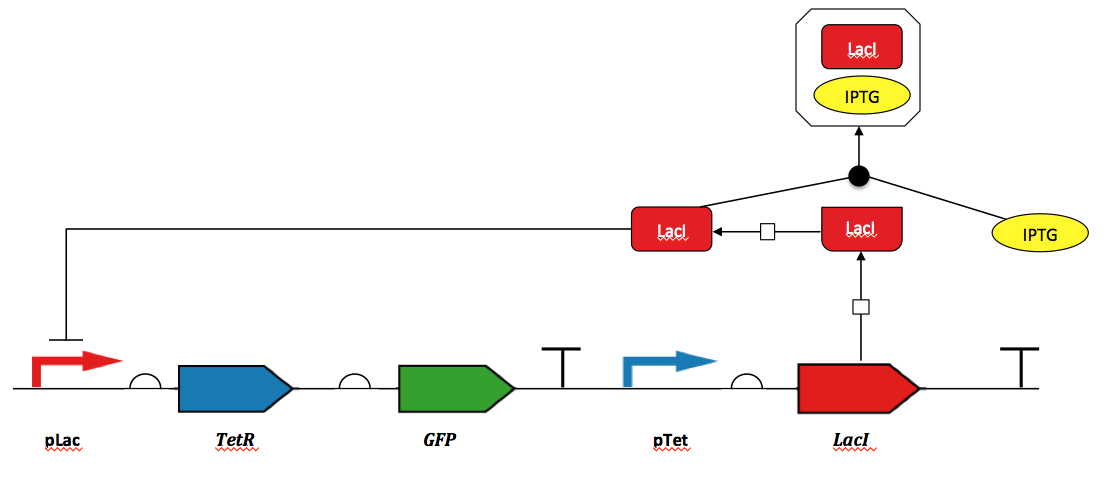
\includegraphics[scale=0.4]{images/toggleswitch_flat}
% \caption[]{An example toggle swicth genetic circuit. }
% \label{images:toggleswitch_flat}
% \end{center}
% \end{figure}

% SBOL includes different entities to describe such genetic circuits. Genetic elements such as promoters, RBS, CDSs and terminators are defined with the \sbol{ComponentDefinition} entity. Their instances are reused in different designs via the \sbol{Component}s that refer to corresponding \sbol{ComponentDefinition}s. \sbol{ComponentDefinition}s can also represent proteins, RNAs or small molecules. They are associated with sequence information such as nucleotides aminoacids or chemical structure. A full description of a genetic circuit is then represented using  \sbol{ModuleDefinition}s which contains information about molecular interactions and their participating components. Modules can be associated with quantitative or qualitative models using the \sbol{Model} entity, which is used to point to the actual location of a model.


% SBOL facilitates the design of complex systems using hierarchical composition. In addition to using simple genetic elements in a modular fashion, modules that are composed of multiple, different components can also be reused. Such modules can expose some of the design components as inputs and outputs, which can be connected to components from other modules using \sbol{MapsTo} entities.

% -----------------------------------------------------------------------------
\section{SBOL Specification Vocabulary}
% -----------------------------------------------------------------------------

This document indicates requirement levels using the controlled vocabulary specified in IETF RFC 2119 and reiterated in BBF RFC 0.
In particular, the key words "MUST", "MUST NOT", "REQUIRED", "SHALL", "SHALL NOT", "SHOULD", "SHOULD NOT", "RECOMMENDED", "MAY", and "OPTIONAL" in this document are to be interpreted as described in RFC 2119.

\begin{itemize}
\item The words "MUST", "REQUIRED", or "SHALL" mean that the item is an absolute requirement.
\item The phrases "MUST NOT" or "SHALL NOT" mean that the item is an absolute prohibition.
\item The word "SHOULD" or the adjective "RECOMMENDED" mean that there may exist valid reasons in particular circumstances to ignore a particular item, but the full implications must be understood and carefully weighed before choosing a different course.
\item The phrases "SHOULD NOT" or "NOT RECOMMENDED" mean that there may exist valid reasons in particular circumstances when the particular behavior is acceptable or even useful, but the full implications should be understood and the case carefully weighed before implementing any behavior described with this label.
\item The word "MAY" or the adjective "OPTIONAL" mean that an item is truly optional.
\end{itemize}

\todo[inline]{Make sure all requirements words are properly upper-cased}

\subsection{SBOL Class Names}

SBOL defines the following classes:

\begin{description}

\item \emph{\sbol{Collection}}:
Represents a user-defined container for organizing a group of SBOL objects.

\item \emph{\sbol{Component}}:
Represents a specific occurrence or instance of a single entity within the design of a more complex component.
Each \sbol{Component} is associated with a \sbol{ComponentDefinition}, and there may be many different instances at different locations in a design that share the same definition.

\item \emph{\sbol{ComponentDefinition}}: Describes the structure of designed entities, such as DNA, RNA, and proteins, as well as other entities they interact with, such as small molecules or environmental properties.

\item \emph{\sbol{FunctionalComponent}}:
Represents a specific occurrence or instance of an entity within a \sbol{ModuleDefinition}.
Exactly like a \sbol{Component}, except that it can be associated with information about its context of use in the \sbol{Module}, rather than in the context of a containing \sbol{ComponentDefinition}.

\item \emph{\sbol{GenericTopLevel}}:
Represents a data container that can contain custom data added by user applications.

\item \emph{\sbol{Interaction}}:
Describes a functional relationship between biological entities, such as regulatory activation or repression, or a biological processes such as transcription or translation.

\item \emph{\sbol{Location}}:
Specifies the base coordinates and orientation of a genetic feature on a DNA or RNA molecule or a residue or site on another sequential macromolecule such as a protein.

\item \emph{\sbol{MapsTo}}:
When a design (\sbol{ComponentDefinition} or \sbol{ModuleDefinition}) includes another design as a substructure, the larger design may need to refer to a \sbol{ComponentInstance} from the sub-design.
In this case, a copy of the referenced \sbol{ComponentInstance} needs to be created in the design and a \sbol{MapsTo} is added to the instance for the sub-design, which associates the original and the copy.

\item \emph{\sbol{Model}}:
Links an SBOL representation of biological components and their interactions to quantitative, computational models that may be used to predict the functional behavior of a biological design.

\item \emph{\sbol{Module}}:
Represents a specific occurrence or instance of a sub-system within a larger design.
Each \sbol{Module} is associated with a \sbol{ModuleDefinition}, and there may be many different instances at different locations in a design that share the same definition.

\item \emph{\sbol{ModuleDefinition}}:
Describes a ``system'' design as a collection of biological components and their functional relationships.

\item \emph{\sbol{Participation}}:
Describes the role that a \sbol{Component} plays in an \sbol{Interaction}.
For example, a transcription factor might participate in an \sbol{Interaction} as a repressor or as an activator.

\item \emph{\sbol{Sequence}}:
Represents a contiguous series of monomers in a macromoleculer polymer such as DNA, RNA, or protein. 

\item \emph{\sbol{SequenceAnnotation}}:
Describes the \sbol{Location} of a notable sub-sequence found within a \sbol{ComponentDefinition}, optionally linking it to a \sbol{Component}.

\item \emph{\sbol{SequenceConstraint}}:
Describes the relative spatial position and orientation of two \sbol{Component} objects that are contained within the same \sbol{ComponentDefinition}.

\end{description}


\section{SBOL Data Model}\label{sec:model}

The section describes the SBOL data model in detail.  Best practices when using the standard can be found in \ref{sec:bestpractices}.

\subsection{Identified}
\label{sec:Identified}

All SBOL-defined classes are directly or indirectly derived from the \sbol{Identified}  abstract class.
This inheritance means that all SBOL objects are uniquely identified using \sbol{URI}s that uniquely refer to these objects within an SBOL document or at locations on the World Wide Web.

As shown in \ref{uml:identified}, the \sbol{Identified} class includes the following properties: \sbol{displayId},  \sbol{name}, \sbol{description}, \sbol{prov:wasDerivedFrom}, and \sbol{prov:wasGeneratedBy}. 

\begin{figure}[ht]
\begin{center}
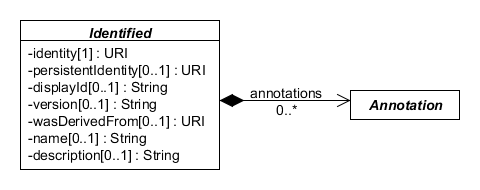
\includegraphics[scale=0.6]{uml/identified}
\caption[]{Diagram of the \sbol{Identified} abstract class and its associated properties}
\label{uml:identified}
\end{center}
\end{figure}
  
\subparagraph{The \sbolheading{displayId} property}
\label{sec:displayId}
The \sbol{displayId} property is an OPTIONAL identifier with a data type of \sbol{String}. This property is intended to be an intermediate between a URI and the \sbol{name} property that is machine-readable, but more human-readable than the full URI of an object.

If the \sbol{displayId} property is used, then its \sbol{String} value MUST be composed of only alphanumeric or underscore characters and MUST NOT begin with a digit.

\subparagraph{The \sbolheading{name} property}
\label{sec:name}

The \sbol{name} property is OPTIONAL and has a data type of \sbol{String}. This property is intended to be displayed to a human when visualizing an \sbol{Identified} object.

If an \sbol{Identified} object lacks a name, then software tools SHOULD instead display the object's \sbol{displayId} or URI.
It is RECOMMENDED that software tools give users the ability to switch perspectives between \sbol{name} properties that are human-readable and \sbol{displayId} properties that are less human-readable, but are more likely to be unique.

\subparagraph{The \sbolheading{description} property}
\label{sec:description}

The \sbol{description} property is OPTIONAL and has a data type of \sbol{String}. This property is intended to contain a more thorough text description of an \sbol{Identified} object.

\subparagraph{The \sbolheading{prov:wasDerivedFrom} property}
\label{sec:prov:wasDerivedFrom}
An \sbol{Identified} object can have zero or more \sbol{prov:wasDerivedFrom} properties, each of type URI. This property is defined by the PROV-O ontology and is located in the \url{https://www.w3.org/TR/prov-o/} namespace (Reference: \ref{sec:provenance}).

 An SBOL object with this property refers to one or more SBOL objects or non-SBOL resources from which this object was derived. An SBOL object MUST NOT refer to itself via its own \sbol{prov:wasDerivedFrom} property or form a cyclical chain of references via its \sbol{prov:wasDerivedFrom} property and those of other SBOL objects. For example, the reference chain ``$A$ was derived from $B$ and $B$ was derived from $A$'' is cyclical.

\subparagraph{The \sbolheading{prov:wasGeneratedBy} property}
\label{sec:prov:wasGeneratedBy}
An \sbol{Identified} object can have zero or more \sbol{prov:wasGeneratedBy} properties, each of type URI. This property is defined by the PROV-O ontology and is located in the \url{https://www.w3.org/TR/prov-o/} namespace (Reference: \ref{sec:provenance}).

An SBOL object with this property refers to one or more \sbol{prov:Activity} objects that describe how this object was generated.
Provenance history formed by \sbol{prov:wasGeneratedBy} properties of \sbol{Identified} objects and entity references in \sbol{prov:Usage} objects MUST NOT form circular reference chains.


\subsection {TopLevel}
\label{sec:TopLevel}
\sbol{TopLevel} is an abstract class that is extended by any \sbol{Identified} class that can be found at the top level of an SBOL document or file. In other words, \sbol{TopLevel} objects are not nested inside any other object via a composite aggregation or black diamond arrow association property. Instead of nesting, composite \sbol{TopLevel} objects refer to subordinate \sbol{TopLevel} objects by their \sbol{URI}s using shared aggregation or white diamond arrow association properties. The \sbol{TopLevel} classes defined in this specification are \sbol{Sequence}, \sbol{Component}, \sbol{Model}, \sbol{Collection}, \sbol{CombinatorialDerivation}, \sbol{Implementation}, \sbol{Attachment}, \sbol{ExperimentalData}, \prov{Activity}, \sbol{prov:Agent}, \\
\sbol{prov:Plan} (see \ref{uml:toplevel}).  Each of these classes is described in more detail below, except for the classes from the provenance ontology (PROV-O), which are described in \ref{sec:provenance}.


\begin{figure}[ht]
\begin{center}
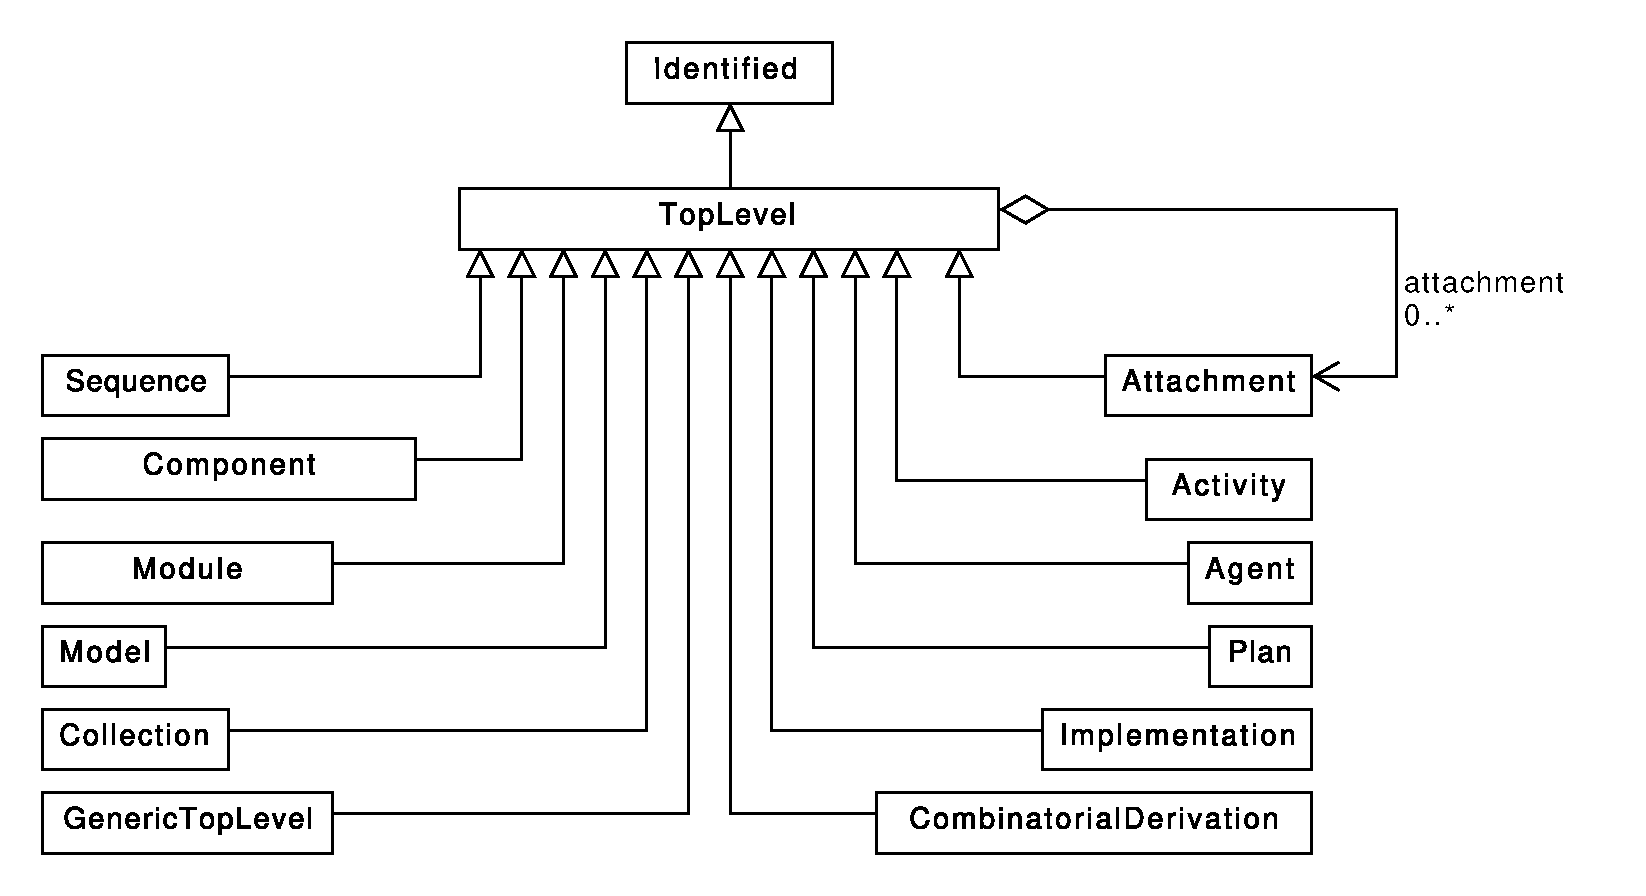
\includegraphics[width=\textwidth]{uml/toplevel}
\caption[]{Classes that inherit from the \sbol{TopLevel} abstract class.}
\label{uml:toplevel}
\end{center}
\end{figure}


\subparagraph{The hasAttachment property}
\label{sec:hasAttachment}
A \sbol{TopLevel} object can have zero or more \sbol{hasAttachment} properties, each of type URI specifying an \sbol{Attachment} object. The \sbol{Attachment} class is described in more detail in Section~\ref{sec:Attachment}.



\subsection{Sequence}
\label{sec:Sequence}
The purpose of the \sbol{Sequence} class is to represent the primary structure of a \sbol{Component} object and the manner in which it is encoded. This representation is accomplished  by means of the \sbol{elements} property and \sbol{encoding} property (\ref{uml:sequence}).

\begin{figure}[ht]
\begin{center}
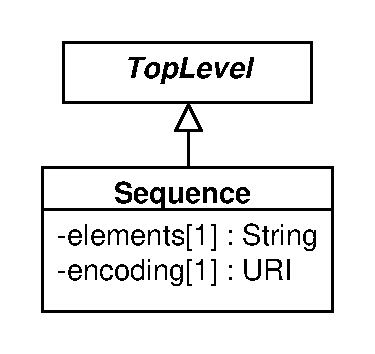
\includegraphics[scale=0.6]{uml/sequence}
\caption[]{Diagram of the \sbol{Sequence} class and its associated properties.}
\label{uml:sequence}
\end{center}
\end{figure}


\subparagraph{The \sbolheading{elements} property}
\label{sec:elements}
The \sbol{elements} property is an OPTIONAL \sbol{String} of characters that represents the constituents of a biological or chemical molecule. 
For example, these characters could represent the nucleotide bases of a molecule of DNA, the amino acid residues of a protein, or the atoms and chemical bonds of a small molecule.

If the \sbol{elements} property is not set, then it means the particulars of this \sbol{Sequence} have not yet been determined.


\subparagraph{The \sbolheading{encoding} property}
\label{sec:encoding}

The \sbol{encoding} property has a data type of \sbol{URI}, and is OPTIONAL unless \sbol{elements} is set, in which case it is REQUIRED.
This property MUST indicate how the \sbol{elements} property of a \sbol{Sequence} are formed and interpreted.
The \sbol{encoding} property SHOULD respectively contain a \sbol{URI} identifying from the textual format (\url{https://identifiers.org/edam:format_2330}) branch of the EDAM ontology.

For example, the \sbol{elements} property of a \sbol{Sequence} with an IUPAC DNA encoding property MUST contain characters that represent nucleotide bases, such as {\tt a}, {\tt t}, {\tt c}, and {\tt g}. The \sbol{elements} property of a \sbol{Sequence} with a Simplified Molecular-Input Line-Entry System (SMILES) encoding, on the other hand, MUST contain characters that represent atoms and chemical bonds, such as {\tt C}, {\tt N}, {\tt O}, and {\tt =}.

\ref{tbl:sequence_encodings} contains a partial list of possible \sbol{URI} values for the \sbol{encoding} property. 
These terms are organized by the type of \sbol{Component} (see \ref{tbl:component_types}) that typically refer to a \sbol{Sequence} with such an \sbol{encoding}. 
It is RECOMMENDED that the encoding property of a Sequence contains a URI from \ref{tbl:sequence_encodings}. 
When the \sbol{encoding} of a \sbol{Sequence} is well described by one of the \sbol{URI}s in \ref{tbl:sequence_encodings}, it MUST contain that \sbol{URI}.

%A Summary of letters for nucleic acids and aminoacids
\begin{table}[ht]
  \begin{edtable}{tabular}{lll}
    \toprule
     \textbf{Encoding} & \textbf{URI} & \textbf{Component Type} \\
    \midrule
     IUPAC DNA, RNA & \url{https://identifiers.org/edam:format_1207} & DNA, RNA \\
    IUPAC Protein & \url{https://identifiers.org/edam:format_1208} & Protein\\
    InChI & \url{https://identifiers.org/edam:format_1197} & Simple Chemical \\
   SMILES & \url{https://identifiers.org/edam:format_1196} & Simple Chemical \\
    \bottomrule
  \end{edtable}
  \caption{\sbol{URI}s for specifying the \sbol{encoding} property of a \sbol{Sequence}, organized by the type of \sbol{Component} (see \ref{tbl:component_types}) that typically refer to a \sbol{Sequence} with such an \sbol{encoding}.}
  \label{tbl:sequence_encodings}
\end{table}


\subsection{Component}
\label{sec:Component}

The \sbol{Component} class represents the structural and/or functional entities of a biological design. The primary usage of this class is to represent entities with designed sequences, such as DNA, RNA, and proteins, but it can also be used to represent any other entity that is part of a design, such as simple chemicals, molecular complexes, strains, samples, light, and abstract functional groupings of other entities.

As shown in \ref{uml:component}, the \sbol{Component} class describes a design entity using the following properties: \sbolmult{type:CD}{type}, \sbolmult{role:CD}{role}, \sbol{hasSequence}, \sbol{hasFeature}, \sbol{hasConstraint}, \sbol{hasInteraction}, and \sbol{hasModel}.  The \sbol{hasSequence}, \sbol{hasFeature}, and \sbol{hasConstraint} properties are used to represent structural relationships, while the \sbol{hasInteraction} and \sbol{hasModel} are used to represent functional relationships.

\begin{figure}[ht]
\begin{center}
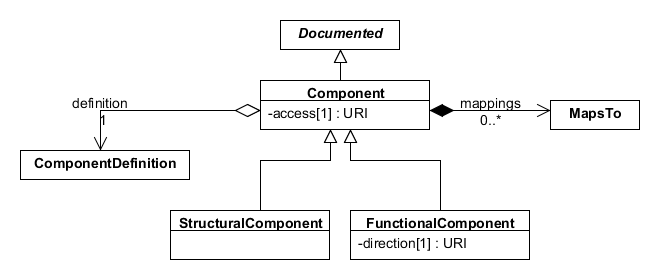
\includegraphics[width=0.95\textwidth]{uml/component}
\caption[]{Diagram of the \sbol{Component} class and its associated properties.}
\label{uml:component}
\end{center}
\end{figure} 

\subparagraph{The \sbolheading{type} property}
\label{sec:type:CD}

A \sbol{Component} is REQUIRED to have one or more \sbolmult{type:CD}{type} properties, each of type \sbol{URI} specifying the category of biochemical or physical entity (for example DNA, protein, or simple chemical) that a \sbol{Component} object abstracts
for the purpose of engineering design. For DNA or RNA entities, additional \sbolmult{type:CD}{type} properties are used to describe nucleic acid topology (circular / linear) and strandedness (double- or single-stranded).

The \sbolmult{type:CD}{type} properties of every \sbol{Component} MUST include one or more \sbol{URI}s that MUST identify terms from appropriate ontologies, such as the physical entity representation branch of the Systems Biology Ontology~\cite{SBO} or the ontology of Chemical Entities of Biological Interest (ChEBI)~\cite{chebi}.  \ref{tbl:component_types} provides a partial list of possible ontology terms for the \sbolmult{type:CD}{type} property and their \sbol{URI}s.  In order to maximize the compatibility of designs, the \sbolmult{type:CD}{type} property of a \sbol{Component} SHOULD contain a \sbol{URI} from the physical entity representation branch of the Systems Biology Ontology~\cite{SBO}, and any \sbol{Component} that can be well-described by one of the terms in \ref{tbl:component_types} MUST use the \sbol{URI} for that term as one of its \sbolmult{type:CD}{type}.
Finally, if the \sbolmult{type:CD}{type} property contains multiple \sbol{URI}s, then they MUST identify non-conflicting terms (otherwise, it might not be clear how to interpret them). For example, the SBO terms provided by \ref{tbl:component_types} would conflict because they specify classes of biochemical entities with different molecular structures.

\begin{table}[ht]
  \begin{edtable}{tabular}{ll}
    \toprule
    \textbf{Component Type} & \textbf{URI for SBO Term} \\
    \midrule
    DNA (Deoxyribonucleic acid)  & \url{https://identifiers.org/SBO:0000251}\\
    RNA (Ribonucleic acid) & \url{https://identifiers.org/SBO:0000250}\\
    Protein (Polypeptide chain)  & \url{https://identifiers.org/SBO:0000252}\\
    Simple Chemical  & \url{https://identifiers.org/SBO:0000247}\\
    Non-covalent complex  & \url{https://identifiers.org/SBO:0000253}\\
    Functional Entity  & \url{https://identifiers.org/SBO:0000241}\\
    \bottomrule
  \end{edtable}
  \caption{Partial list of the most common SBO terms to specify the molecule type using the \sbolmult{type:CD}{type} property of a \sbol{Component}.  Systems composed of multiple molecules composed together to perform a function should use the functional entity type.}
 \label{tbl:component_types}
\end{table}

\emph{Nucleic Acid Topology types}\\
Any \sbol{Component} classified as DNA (see \ref{tbl:component_types}) is RECOMMENDED to encode circular/linear topology information in an additional type field. This (topology) type field SHOULD specify a URI from the Topology Attribute branch of the SO
(this is currently just `linear' or `circular' as given in \ref{tbl:component_topology}). Topology information SHOULD be specified for DNA \sbol{Component} records with a fully specified sequence, except in three scenarios: if the DNA record does not have sequence information, or if the DNA record has incomplete sequence information, or if topology is genuinely unknown. For any \sbol{Component} classified as RNA (see \ref{tbl:component_types}), a topology type field is OPTIONAL. The default
assumption in this case is linear topology.  In any case, no more than one topology should be specified.

Any \sbol{Component} classified as DNA or RNA MAY also have strand
information encoded in an additional (third) type field using a URI from the Strand Attribute branch of the SO (currently there are only two possible terms for single or double-stranded nucleic
acids given in \ref{tbl:component_topology}). In absence of this field, the
default strand information assumed for DNA is `double-stranded' and for RNA is
`single-stranded'. 

Any other type of \sbol{Component} record (protein, simple chemical, etc) SHOULD NOT
have any type field pointing to SO terms from the topology or strand attribute branches of SO.

Note that a \emph{circular} topology instructs software to interpret the
beginning / end position of a given sequence (be it DNA or RNA) as arbitrary so
that sequence features may be mapped or identified across this junction. \emph{Double stranded} instructs software to apply sequence searches to both strands (i.e. sequence and reverse complement of sequence).

\begin{table}[ht]
  \begin{edtable}{tabular}{ll}
    \toprule
    \textbf{Nucleic Acid Topology} & \textbf{URI for Nucleic Acid Topology
      Term in SO} \\
    \midrule
    linear  & \url{http://identifiers.org/so/SO:0000987}\\
    circular  & \url{http://identifiers.org/so/SO:0000988}\\
    single-stranded & \url{http://identifiers.org/so/SO:0000984}\\
    double-stranded & \url{http://identifiers.org/so/SO:0000985}\\
    \bottomrule
  \end{edtable}
  \caption{Sequence Ontology terms to encode DNA or RNA topology information in the \sbolmult{types:CD}{types} properties of a \sbol{Component}.}
 \label{tbl:component_topology}
\end{table}

\subparagraph{The \sbolheading{role} property}
\label{sec:role:CD}

A \sbol{Component} MAY have one or more \sbolmult{role:CD}{role} properties, each of type \sbol{URI} that MUST identify terms from ontologies that are consistent with the \sbolmult{type:CD}{type} property of the \sbol{Component}.  For example, the \sbolmult{role:CD}{role} property of a DNA or RNA \sbol{Component} could contain URIs identifying terms from SO. As a best practice, a DNA or RNA \sbol{Component} SHOULD contain exactly one \sbol{URI} that refers to a term from the sequence feature branch of the SO.
Similarly, the role properties of a protein and simple chemical \sbol{Component} SHOULD respectively contain \sbol{URI}s identifying terms from the \texttt{MolecularFunction} branch (\texttt{GO:0003674}) of the Gene Ontology (GO) and the \texttt{role} branch (\texttt{CHEBI:50906}) of the CHEBI ontology.
\ref{tbl:component_roles} contains a partial list of possible ontology terms for the \sbolmult{role:CD}{role} properties and their \sbol{URI}s. These terms are organized by the type of \sbol{Component} to which they SHOULD apply (see \ref{tbl:component_types}). Any \sbol{Component} that can be well-described by one of the terms in \ref{tbl:component_roles} MUST use the \sbol{URI} for that term as one of its \sbolmult{role:CD}{role}.

These \sbol{URI}s might identify descriptive biological roles, such as ``metabolic pathway'' and ``signaling cascade,'' but they can also identify identify ``logical'' roles, such as ``inverter'' or ``AND gate'', or other abstract roles for describing the function of design. Interpretation of the meaning of such roles currently depends on the software tools that read and write them.

\begin{table}[ht]
  \begin{edtable}{tabular}{lll}
    \toprule
    \textbf{Component Role} & \textbf{URI for Ontology Term} & \textbf{Component Type} \\
    \midrule
   Promoter & \url{http://identifiers.org/so/SO:0000167} & DNA \\
   RBS & \url{http://identifiers.org/so/SO:0000139} & DNA \\
      CDS & \url{http://identifiers.org/so/SO:0000316} & DNA \\
      Terminator & \url{http://identifiers.org/so/SO:0000141} & DNA \\
      Gene & \url{http://identifiers.org/so/SO:0000704} & DNA \\
      Operator & \url{http://identifiers.org/so/SO:0000057} & DNA \\
      Engineered Gene & \url{http://identifiers.org/so/SO:0000280} & DNA \\
      mRNA & \url{http://identifiers.org/so/SO:0000234} & RNA \\
      Effector & \url{http://identifiers.org/chebi/CHEBI:35224} & Small Molecule \\
      Transcription Factor & \url{http://identifiers.org/go/GO:0003700} & Protein\\
    \bottomrule
  \end{edtable}
  \caption{Partial list of ontology terms to specify the \sbolmult{role:CD}{role} property of a \sbol{Component}, organized by the type of \sbol{Component} to which they are intended to apply (see \ref{tbl:component_types}).}
  \label{tbl:component_roles}
\end{table}

\subsubsection*{The \sbolheading{hasSequence} property}
\label{sec:hasSequence}
A \sbol{Component} MAY have one or more \sbol{hasSequence} properties, each of type \sbol{URI} that MUST reference a \sbol{Sequence} object (see \ref{sec:Sequence}).  These objects define the primary structure of the \sbol{Component}.

If a \sbol{Feature} of a \sbol{Component} refers to a \sbol{Location}, and this \sbol{Location} refers to a \sbol{Sequence}, then the \sbol{Component} MUST also include a \sbol{hasSequence} property that refers to this \sbol{Sequence}.

Many \sbol{Component} objects will have exactly one \sbol{hasSequence} property that refers to a \sbol{Sequence} object.  In this case, if its has a \sbolmult{type:CD}{type} from \ref{tbl:componentdefinition_types} and there is an \sbol{encoding} that is cross-listed with this term in \ref{tbl:sequence_encodings}, then the \sbol{Sequence} objects MUST have this encoding.
This \sbol{Sequence} is implicitly the entire sequence for this \sbol{Component} (In other words, it is equivalent to a \sbol{SequenceFeature} with an \sbol{EntireSequence} \sbol{Location} that refers to this \sbol{Sequence}).

\subparagraph{The \sbolheading{hasFeature} property}
\label{sec:hasFeature}

A \sbol{Component} MAY have one or more \sbol{hasFeature} properties, each of type \sbol{URI} that MUST reference a \sbol{Feature} object (see \ref{sec:Feature}). The set of relations between \sbol{Feature} and \sbol{Component} objects MUST be strictly acyclic.

While the \sbol{Component} class is analogous to a blueprint or specification sheet for a biological part or a system of interacting biological elements, the \sbol{Feature} class represents, among other things, the specific occurrence of a part or subsystem within a design.  For example, this mechanism allows a biological design to include multiple instances of a particular part (defined by reference to the same \sbol{Component}). For example, the \sbol{Component} of a polycistronic gene could contain two \sbol{SubComponent} objects that refer to the same \sbol{Component} of a CDS.  As another example, consider the \sbol{Component} for a network of two-input repressor devices in which the particular repressors have not been chosen yet. This \sbol{Component} could contain multiple \sbol{SubComponent} objects that refer to the same \sbol{Component} of an abstract two-input repressor device.

The \sbol{hasFeature} properties of \sbol{Component} objects can be used to construct a hierarchy of \sbol{SubComponent} and \sbol{Component} objects.  If a \sbol{Component} in such a hierarchy refers to a \sbol{Location} object, and there exists a \sbol{Component} object lower in the hierarchy that refers to a \sbol{Location} object that refers to the same \sbol{Sequence} with the same \sbol{encoding}, then the \sbol{elements} properties of these \sbol{Sequence} objects SHOULD be consistent with each other, such that well-defined mappings exist from the ``lower level'' \sbol{elements} to the ``higher level'' \sbol{elements} in accordance with their shared \sbol{encoding} properties. This mapping is also subject to any restrictions on the positions of the \sbol{Feature} objects in the hierarchy that are imposed by the \sbol{SubComponent}, \sbol{SequenceFeature}, or \sbol{SequenceConstraint} objects contained by the \sbol{Component} objects in the hierarchy.

A DNA \sbol{Component}, for example, could refer to a \sbol{Sequence} with an \external{IUPAC DNA} \sbol{encoding} and an \sbol{elements} \external{String} of ``{\tt gattaca}.'' In turn, this \sbol{Component} could contain a \sbol{SubComponent} that refers to a ``lower level''  \sbol{Component} that also refers to a \sbol{Sequence} with an \external{IUPAC DNA} \sbol{encoding}. Consequently, a consistent \sbol{elements} \external{String} of this ``lower level'' \sbol{Sequence} could be ``{\tt gatta},'' or perhaps ``{\tt tgta}'' if the \sbol{SubComponent} is positioned by a \sbol{Location} with an \sbol{orientation} of ``reverse complement'' (see \ref{sec:Location}).

\subparagraph{The \sbolheading{hasConstraint} property}
\label{sec:hasConstraint}

A \sbol{Component} MAY have one or more \sbol{hasConstraint} properties, each of type \sbol{URI} that MUST reference a \sbol{Constraint} object (see \ref{sec:Constraint}).  These objects describe, among other things, any restrictions on the relative, sequence-based positions and/or orientations of the \sbol{Feature} objects contained by the \sbol{Component}.
For example, the \sbol{Component} of a gene might specify that the position of its promoter \sbol{SubComponent} precedes that of its CDS \sbol{SubComponent}. This is particularly useful when a \sbol{Component} lacks a \sbol{Sequence} and therefore cannot specify the precise, sequence-based positions of its \sbol{SubComponent} objects using \sbol{Location} objects.

\subparagraph{The \sbolheading{hasInteraction} property}\label{sec:hasInteraction}

A \sbol{Component} MAY have one or more \sbol{hasInteraction} properties, each of type \sbol{URI} that MUST reference an \sbol{Interaction} object (see \ref{sec:Interaction}).  

The \sbol{Interaction} class provides an abstract, machine-readable representation of entity behavior within a \sbol{Component} (whereas a more detailed model of the system might not be suited to machine reasoning, depending on its implementation).
Each \sbol{Interaction} contains \sbol{Participation} objects that indicate the roles of the \sbol{Feature} objects involved in the \sbol{Interaction}.

\subparagraph{The \sbolheading{hasModel} property}\label{sec:hasModel}

A \sbol{Component} MAY have one or more \sbol{hasModel} properties, each of type \sbol{URI} that MUST reference a \sbol{Model} object (see \ref{sec:Model}).  

\sbol{Model} objects are placeholders that link \sbol{Component} objects to computational models of any format.
A \sbol{Component} object can link to more than one \sbol{Model} since each might encode system behavior in a different way or at a different level of detail.

\subsubsection{Feature}
\label{sec:Feature}

\begin{figure}[ht]
\begin{center}
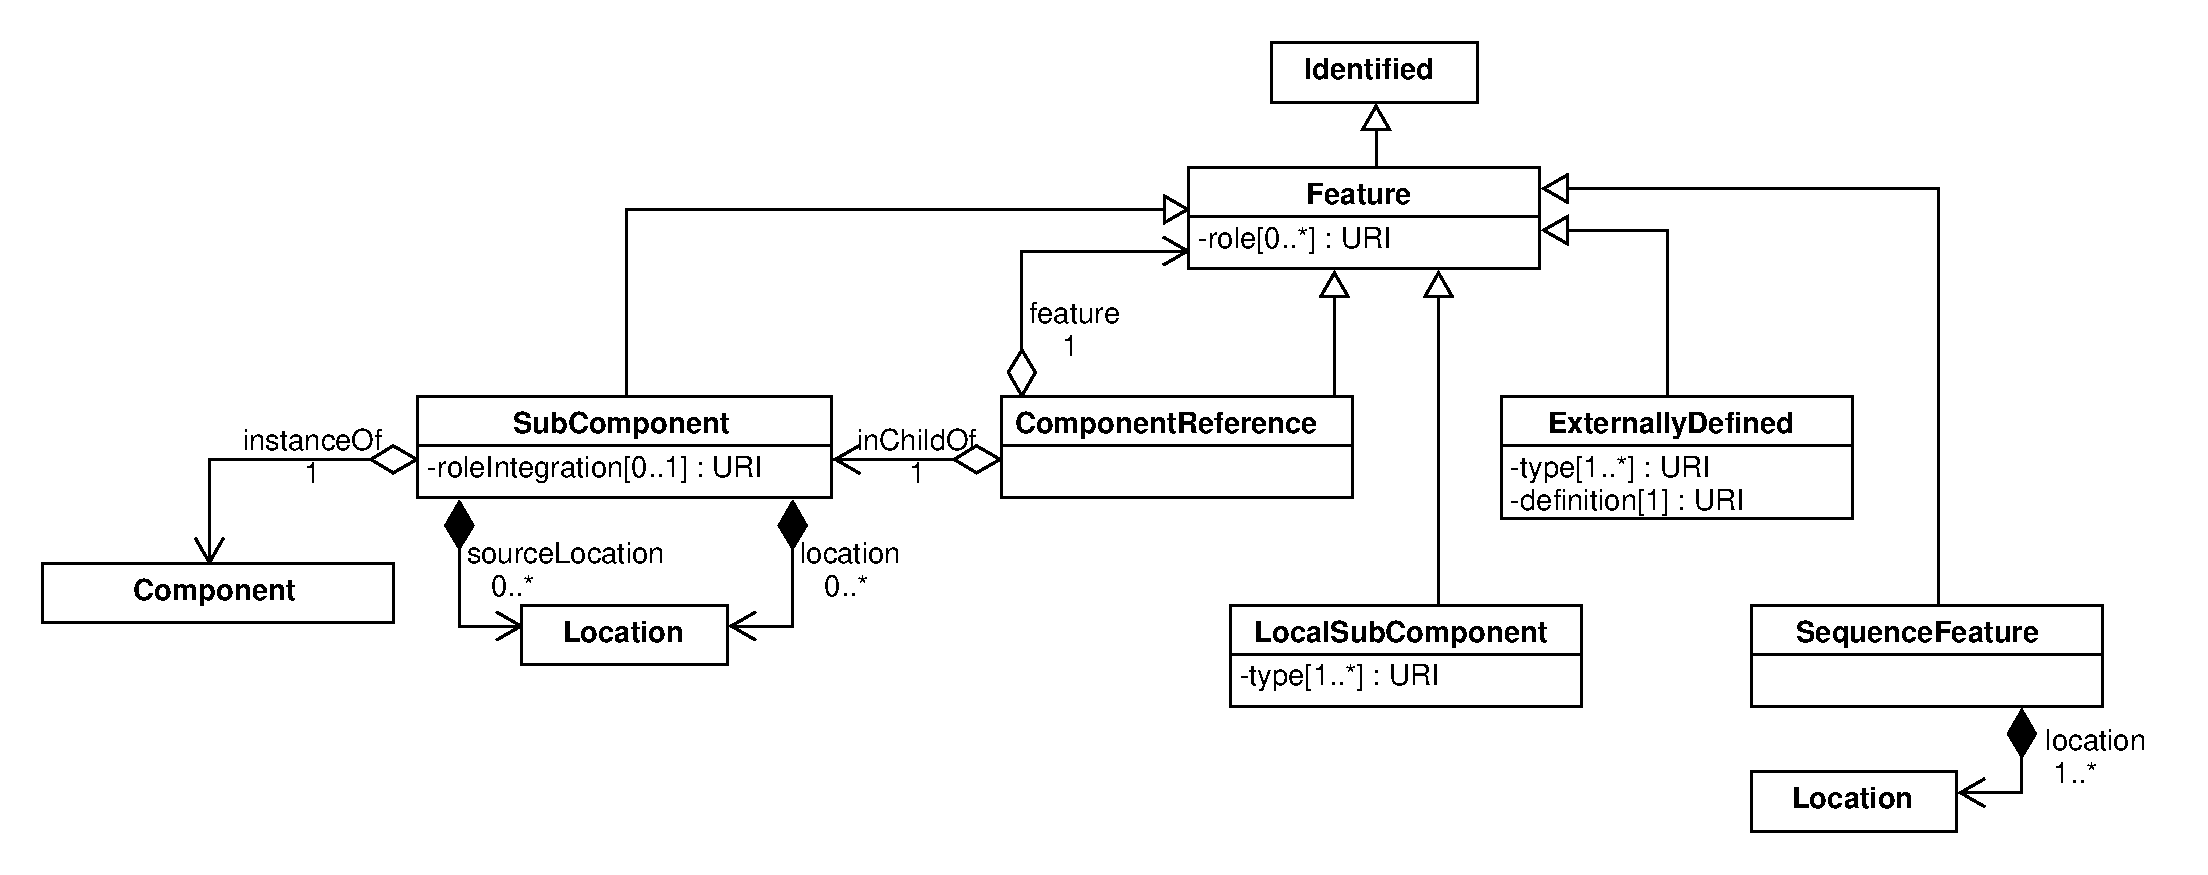
\includegraphics[width=\textwidth]{uml/feature}
\caption[]{Diagram of the \sbol{Feature} class and its associated properties.}
\label{uml:subcomponent}
\end{center}
\end{figure}

The \sbol{Feature} class is used to compose \sbol{Component} objects into a structural or functional hierarchy. 

\subparagraph{The \sbolheading{role} property}\label{sec:roles:C}

The expected purpose and function of a genetic part are described by the
\sbolmult{roles:CD}{roles} property of \sbol{Component}. However, the same building block might be used for a different purpose in an actual design. In other words, purpose and function are sometimes determined by context. 

The \sbolmult{roles:C}{roles} property comprises an OPTIONAL set of zero or more \sbolmult{roles:C}{role} \sbol{URI}s describing the purpose or potential function of this \sbol{Feature}'s included sub-\sbol{Component} in the \textit{context} of its parent \sbol{Component}.
If provided, these \sbolmult{roles:C}{role} \sbol{URI}s MUST identify terms from appropriate ontologies. Roles are not restricted to describing biological function; they may annotate a \sbol{Feature}'s function in any domain for which an ontology exists.

It is RECOMMENDED that these \sbolmult{roles:C}{role} \sbol{URI}s identify terms that are compatible with the \sbolmult{types:CD}{type} properties of both this \sbol{Feature}'s parent \sbol{Component} and its included sub-\sbol{Component}. For example, a \sbolmult{roles:C}{role} of a \sbol{Feature} which belongs to a \sbol{Component} of type DNA and includes a sub-\sbol{Component} of type DNA might refer to terms from the Sequence Ontology. A table of recommended ontology terms for \sbolmult{roles:C}{roles} is given in \ref{tbl:component_roles}.

\paragraph{SubComponent}
\label{sec:SubComponent}

The \sbol{SubComponent} class a subclass of the \sbol{Feature} class that can be used to specify structural hierarchy. For example, the \sbol{Component} of a gene could contain four \sbol{SubComponent} objects: a promoter, RBS, CDS, and terminator. In turn, the \sbol{Component} of the promoter \sbol{SubComponent} could contain \sbol{SubComponent} objects defined as various operator sites.

\subparagraph{The \sbolheading{roleIntegration} property}\label{sec:roleIntegration:C}


A \sbolmult{roleIntegration:C}{roleIntegration} specifies the relationship between a \sbol{Feature} instance's own set of \sbolmult{roles:C}{roles} and the set of \sbolmult{roles:CD}{roles} on the included sub-\sbol{Component}.

The \sbolmult{roleIntegration:C}{roleIntegration} property has a data type of \sbol{URI}. A \sbol{Feature} instance with zero \sbolmult{roles:C}{roles} MAY OPTIONALLY specify a \sbolmult{roleIntegration:C}{roleIntegration}. A \sbol{Feature} instance with one or more \sbolmult{roles:C}{roles} MUST specify a \sbolmult{roleIntegration:C}{roleIntegration} from \ref{tbl:component_roleIntegration}.
If zero \sbol{Feature} \sbolmult{roles:C}{roles} are given and no \sbol{Feature} \sbolmult{roleIntegration:C}{roleIntegration} is given, then \url{http://sbols.org/v2\#mergeRoles} is assumed.
It is RECOMMENDED to specify a set of \sbol{Feature} \sbolmult{roles:C}{roles} only if the integrated result set of roles would differ from the set of \sbolmult{roles:CD}{roles} belonging to this \sbol{Feature}'s included sub-\sbol{Component}.


\begin{table}[ht]
  \begin{edtable}{tabular}{lp{4in}}
    \toprule
    \textbf{roleIntegration URI} & \textbf{Description} \\
    \midrule
    \url{http://sbols.org/v2\#overrideRoles} & In the context of this \sbol{Feature}, ignore any \sbolmult{roles:CD}{roles} given for the included sub-\sbol{Component}. Instead use only the set of zero or more \sbolmult{roles:C}{roles} given for this \sbol{Feature}. \\
    \url{http://sbols.org/v2\#mergeRoles} & Use the union of the two sets: both the set of zero or more \sbolmult{roles:C}{roles} given for this \sbol{Feature} as well as the set of zero or more \sbolmult{roles:CD}{roles} given for the included sub-\sbol{Component}. \\
    \bottomrule
  \end{edtable}
  \caption{Each \sbolmult{roleIntegration:C}{roleIntegration} mode is associated with a rule governing how a \sbol{Feature}'s roles are to be combined with the included 
sub-\sbol{Component}'s roles.}
  \label{tbl:component_roleIntegration}
\end{table}


\subparagraph{The \sbolheading{instanceOf} property}
\label{sec:instanceOf}

The \sbol{instanceOf} property is a REQUIRED \sbol{URI} that refers to the \sbol{Component} of the \sbol{Feature}.
As described in the previous section, this \sbol{Component} effectively provides information about the \sbolmult{types:CD}{types} and \sbolmult{roles:CD}{roles} of the \sbol{Feature}.

The \sbol{instanceOf} property MUST NOT refer to the same \sbol{Component} as the one that contains the \sbol{Feature}.
Furthermore, \sbol{Feature} objects MUST NOT form a cyclical chain of references via their \sbol{instanceOf} properties and the \sbol{Component} objects that contain them.
For example, consider the \sbol{Feature} objects $A$ and $B$ and the \sbol{Component} objects $X$ and $Y$. The reference chain ``$X$ contains $A$, $A$ is defined by $Y$, $Y$ contains $B$, and $B$ is defined by $X$'' is cyclical.

The \sbol{sourceLocations} property is an OPTIONAL set of zero or more \sbol{Location} objects that indicate which \sbol{elements} of a \sbol{Component}'s \sbol{Sequence} are to be included in the \sbol{Component}'s parent. The \sbol{sourceLocations} property
allows for only a portion of a \sbol{Component}'s \sbol{Sequence} to be included, rather than its entirety.

If the \sbol{sourceLocation} property is not set, then the whole \sbol{Sequence} is assumed to be included. Alternatively,
if the \sbol{sourceLocation} property is set, then the relationship between the original \sbol{Component}'s
\sbol{Sequence} and the included \sbol{Sequence} is defined identically to the \sbol{locations}
property on the \sbol{SequenceFeature} object.


\subparagraph{The \sbolheading{location} property}\label{sec:location}
The \sbol{location} property is an OPTIONAL set which points to a \sbol{Location} on the parent \sbol{Component} sequence; if \sbol{location} is missing, this indicates a part / sub-part relationship for which sequence details have not (yet) been determined.

The \sbol{Location} record(s) specified by a \sbol{Feature} are subject to the same restrictions currently in place for \sbol{SequenceFeature} \sbol{Location}. Concretely, two \sbol{Location} records attached to the same \sbol{Feature} MUST NOT overlap in their range as it would not be clear what that means. The \sbol{Location} of two separate \sbol{Feature}s may overlap.

\subparagraph{The \sbolheading{orientation} property}\label{sec:orientation2}
The \sbol{orientation} property is OPTIONAL and has a data type of \sbol{URI}. All subclasses of \sbol{Feature} share this property, which can be used to indicate how the region specified by the \sbol{SequenceFeature} and any associated double-stranded \sbol{SubComponent} is oriented on the \sbol{elements} of a \sbol{Sequence}  from their parent \sbol{Component}. \ref{tbl:orientation_types} provides a list of REQUIRED \sbol{orientation} \sbol{URI}s. If a \sbol{Feature} object has an \sbol{orientation}, then it MUST come from \ref{tbl:orientation_types}.

\todo{add best practice here talking about EntireComponent?}


\paragraph{ComponentReference}
\label{sec:ComponentReference}

The \sbol{ComponentReference} class is a subclass of \sbol{Feature} and a sibling of the \sbol{SubComponent} class. 


\subparagraph{The \sbolheading{inChildOf} property}\label{sec:inChildOf}

The \sbol{inChildOf} property is a REQUIRED \sbol{URI} that refers to a SubComponent. \sbol{inChildOf} must refer to a \sbol{SubComponent} pointed directly to by the parent of the \sbol{ComponentReference} (i.e., as a \sbol{SubComponent} of \sbol{Component}, or an \sbol{inChildOf} of \sbol{ComponentReference}). If the \sbol{Feature} is a \sbol{SubComponent}, then it must be a child of the \sbol{SubComponent} pointed to by \sbol{inChildOf}.

\subparagraph{The \sbolheading{feature} property}\label{sec:feature:CR}

The \sbolmult{feature:CR}{feature} property is an OPTIONAL \sbol{URI} that refers to a \sbol{Feature}.

\paragraph{LocalSubComponent}
\label{sec:LocalSubComponent}

The \sbol{LocalSubComponent} class a subclass of \sbol{Feature}. This class was serves as a way to create an ``empty'' \sbol{Component} to serve as a placeholder in more complex \sbol{Component}s. 

\subparagraph{The \sbolheading{type} property}\label{sec:type:LSC}

The \sbolmult{type:LSC}{type} property is REQUIRED and contains one or more \sbol{URI}s. The \sbolmult{type:LSC}{type} property is identical to its use in \sbol{Component}

\paragraph{ExternallyDefined}
\label{sec:ExternallyDefined}

The \sbol{ExternallyDefined} class has been introduced so that external definitions in databases like CHEBI or UniProt can be referenced.

\subparagraph{The \sbolheading{type} property}\label{sec:type:ED}

The \sbolmult{type:ED}{type} property is REQUIRED and contains one or more \sbol{URI}s. The \sbolmult{type:ED}{type} property is identical to its use in \sbol{Component}

\subparagraph{The \sbolheading{definition} property}\label{sec:definition:ER}

The \sbolmult{definition:ER}{definition} property is REQUIRED and contains one \sbol{URI} that links to a cononical definition external to SBOL.


\paragraph{SequenceFeature}
\label{sec:SequenceFeature}

The \sbol{SequenceFeature} class describes one or more regions of interest on the \sbol{Sequence} objects referred to by its parent \sbol{Component}. 
%In addition, \sbol{SequenceFeature} objects can describe the substructure of their parent \sbol{Component} through association with the \sbol{Feature} objects contained by this \sbol{Component}.

\subparagraph{The \sbolheading{locations} property}\label{sec:locations}
The \sbol{locations} property is a REQUIRED set of one or more \sbol{Location} objects that indicate which \sbol{elements} of a \sbol{Sequence} are described by the \sbol{SequenceFeature}.

Allowing multiple \sbol{Location} objects on a single \sbol{SequenceFeature} is intended to enable representation of discontinuous regions (for example, a \sbol{Feature} encoded across a set of exons with interspersed introns).
As such, the \sbol{Location} objects of a single \sbol{SequenceFeature} SHOULD NOT specify overlapping regions, since it is not clear what this would mean.
There is no such concern with different \sbol{SequenceFeature} objects, however, which can freely overlap in \sbol{Location} (for example, specifying overlapping linkers for sequence assembly).

\subsubsection{Location}
\label{sec:Location}
The \sbol{Location} class is extended by the \sbol{Range}, \sbol{Cut}, and \sbol{EntireSequence} classes.

\begin{figure}[ht]
\begin{center}
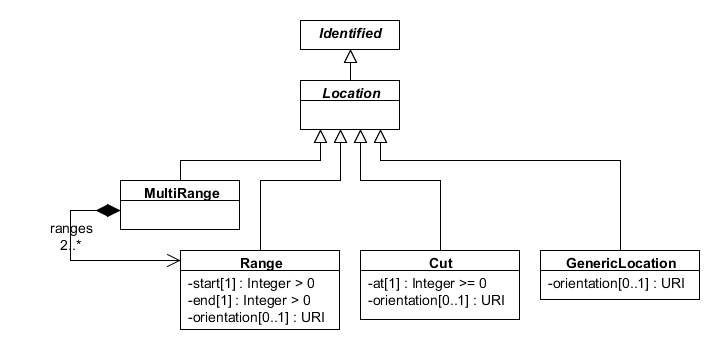
\includegraphics[scale=0.6]{uml/location}
\caption[]{Diagram of the \sbol{Location} class and its associated properties.}
\label{uml:location}
\end{center}
\end{figure} \todo{change diagram to reflect changes from SEP 41}

\subparagraph{The \sbolheading{orientation} property}
\label{sec:orientation}
The \sbol{orientation} property is OPTIONAL and has a data type of \sbol{URI}. All subclasses of \sbol{Location} share this property, which can be used to indicate how the region specified by the \sbol{SequenceFeature} and any associated double-stranded \sbol{Feature} is oriented on the \sbol{elements} of a \sbol{Sequence}  from their parent \sbol{Component}. \ref{tbl:orientation_types} provides a list of REQUIRED \sbol{orientation} \sbol{URI}s. If a \sbol{Location} object has an \sbol{orientation}, then it MUST come from \ref{tbl:orientation_types}.

\subparagraph{The \sbolheading{sequence} property}
\label{sec:sequence}
The \sbol{sequence} property is REQUIRED and MUST contain the \sbol{URI} of a \sbol{Sequence} object. All subclasses of \sbol{Location} share this property, which indicates which \sbol{Sequence} object referenced by the containing \sbol{Component} is referenced by the \sbol{Location}.

\begin{table}[ht]
  \begin{edtable}{tabular}{lp{3.75in}}
    \toprule
    \textbf{Orientation URI} & \textbf{Description} \\
    \midrule
    \url{http://sbols.org/v2\#inline} & The region specified by this \sbol{Location} is on the \sbol{elements} of a \sbol{Sequence}. \\
    \url{http://sbols.org/v2\#reverseComplement} & The region specified by this \sbol{Location} is on the reverse-complement translation of the \sbol{elements} of a \sbol{Sequence}. The exact nature of this translation depends on the \sbol{encoding} of the \sbol{Sequence}. \\
    \bottomrule
  \end{edtable}
  \caption{REQUIRED \sbol{URI}s for the \sbol{orientation} property}
  \label{tbl:orientation_types}
\end{table}


\paragraph{Range}
\label{sec:Range}
A \sbol{Range} object specifies a region via discrete, inclusive \sbol{start} and \sbol{end} positions that correspond to indices for characters in the \sbol{elements} \sbol{String} of a \sbol{Sequence}.

Note that the index of the first location is 1, as is typical practice in biology, rather than 0, as is typical practice in computer science.

\subparagraph{The \sbolheading{start} property}\label{sec:start}
The \sbol{start} property specifies the inclusive starting position of the \sbol{Range}. This property is REQUIRED and MUST contain an \sbol{Integer} value greater than zero.

\subparagraph{The \sbolheading{end} property}\label{sec:end}
The \sbol{end} property specifies the inclusive ending position of the \sbol{Range}. This property is REQUIRED and MUST contain an \sbol{Integer} value greater than zero. In addition, this \sbol{Integer} value MUST be greater than or equal to that of the \sbol{start} property.

\paragraph{Cut}
\label{sec:Cut}
The \sbol{Cut} class has been introduced to enable the specification of a region between two discrete positions.
This specification is accomplished using the \sbol{at} property, which specifies a discrete position that that corresponds to the index of a character in the \sbol{elements} \sbol{String} of a \sbol{Sequence} (except in the case when \sbol{at} is equal to zero---see below).

\subparagraph{The \sbolheading{at} property}
\label{sec:at}
The \sbol{at} property is REQUIRED and MUST contain an \sbol{Integer} value greater than or equal to zero. The region specified by the \sbol{Cut} is between the position specified by this property and the position that immediately follows it. When the \sbol{at} property is equal to zero, the specified region is immediately before the first discrete position or character in the \sbol{elements} \sbol{String} of a \sbol{Sequence}.


\paragraph{EntireSequence}
\label{sec:EntireSequence}
The \sbol{EntireSequence} class does not have any additional properties. Use of this class indicates that the linked Sequence describes the entirety of the \sbol{Component} or \sbol{Feature} parent of this Location object.

\subparagraph{The \sbolheading{order} property}
\label{sec:order}


\subsubsection{Constraint}
\label{sec:Constraint}
The \sbol{Constraint} class can be used to assert restrictions on the relationships of pairs of \sbol{Feature} objects contained by the same parent \sbol{Component}.
Uses of this class include expressing containment (e.g., a plasmid transformed into a chassis strain), identity mappings (e.g., replacing a placeholder value with a complete definition), and expressing relative, sequence-based positions (e.g., the ordering of features within a template).
Each \sbol{Constraint} includes the \sbol{restriction}, \sbol{subject}, and \sbol{object} properties.

\begin{figure}[ht]
\begin{center}
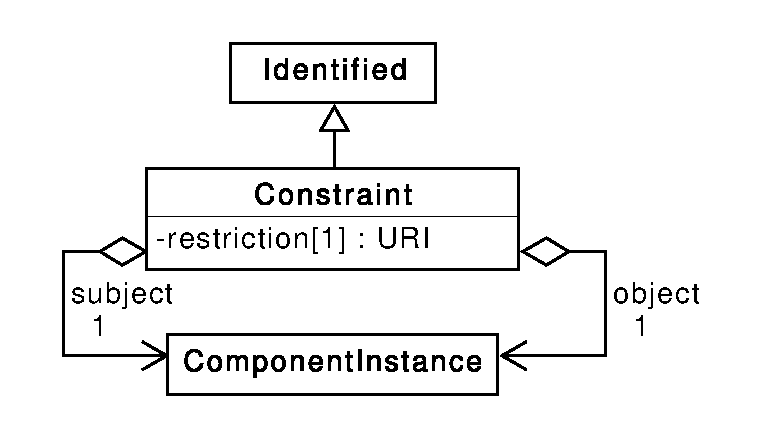
\includegraphics[scale=0.6]{uml/constraint}
\caption[]{Diagram of the \sbol{Constraint} class and its associated properties.}
\label{uml:sequence_constraint}
\end{center}
\end{figure}

\subparagraph{The \sbolheading{subject} property}\label{sec:subject}
The \sbol{subject} property is REQUIRED and MUST contain a \sbol{URI} that refers to a \sbol{Feature} contained by the same parent \sbol{Component} that contains the \sbol{Constraint}.

\subparagraph{The \sbolheading{object} property}\label{sec:object}
The \sbol{object} property is REQUIRED and MUST contain a \sbol{URI} that refers to a \sbol{Feature} contained by the same parent \sbol{Component} that contains the \sbol{Constraint}. This \sbol{Feature} MUST NOT be the same \sbol{Feature} that the \sbol{Constraint} refers to via its \sbol{subject} property.

\subparagraph{The \sbolheading{restriction} property}\label{sec:restriction}

The \sbol{restriction} property is REQUIRED and has a data type of \sbol{URI}. 
This property MUST indicate the type of restriction on the locations, orientations, or identities of the \sbol{subject} and \sbol{object} \sbol{ComponentInstance} objects in relation to each other. 
The \sbol{URI} value of this property SHOULD come from the RECOMMENDED \sbol{URI}s in \ref{tbl:restriction_types_identity}, \ref{tbl:restriction_types_topology}, and \ref{tbl:restriction_types_sequence}.

% identify and orientation
\begin{table}[ht]
  \begin{edtable}{tabular}{lp{3.25in}}
    \toprule
    \textbf{Restriction URI} & \textbf{Description} \\
    \midrule
    % identity relations
	\url{http://sbols.org/v3#verifyIdentical}  & The \sbol{instanceOf} properties of the \sbol{subject} and \sbol{object} \sbol{Feature} objects MUST refer to the same \sbol{Component}.  \emph{Example: a promoter included via two different subsystems must be the identical.} \\
	\url{http://sbols.org/v3\#differentFrom} & The \sbol{instanceOf} property of the \sbol{subject} \sbol{Feature} MUST NOT refer to the same \sbol{Component} as that of the \sbol{object} \sbol{Component}. \emph{Example: two fluorescent reporters must be different.}\\
	\url{http://sbols.org/v3#replaces} &	In the context of the parent object of the \sbol{Constraint}, information about the \sbol{subject} should be used in place of all instances of the \sbol{object}. \emph{Example: the J23101 promoter replaces a generic promoter.} \\
    
    % orientation relations
	\url{http://sbols.org/v3\#sameOrientationAs} & The \sbol{subject} and \sbol{object} \sbol{Component} objects MUST have the same orientation. \emph{Example: a promoter has the same orientation as the coding sequence it controls.}\\
	\url{http://sbols.org/v2\#oppositeOrientationAs} & The \sbol{subject} and \sbol{object} \sbol{Component} objects MUST have opposite orientations. \emph{Example: a promoter has the opposite orientation as an invertase-activated coding sequence it controls.}\\

    \bottomrule
  \end{edtable}
  \caption{RECOMMENDED \sbol{URI}s for expressing identity and orientation with the \sbol{restriction} property.}
  \label{tbl:restriction_types_identity}
\end{table}

    % topology relations
\begin{table}[ht]
  \begin{edtable}{tabular}{lp{3.25in}}
    \toprule
    \textbf{Restriction URI} & \textbf{Description} \\
    \midrule
	\url{http://sbols.org/v3#isDisjointFrom}	& The \sbol{subject} and \sbol{object} do not overlap in space. \emph{Example: a plasmid is disjoint from a chromosome.} \\
	\url{http://sbols.org/v3#strictlyContains} &	The \sbol{subject} entirely contains the \sbol{object}: they do not share a boundary. \emph{Example: a cell contains a plasmid} \\
	\url{http://sbols.org/v3#contains} &	The \sbol{subject} contains the \sbol{object} and they might or might not share a boundary (i.e., union of {\tt strictlyContains}, {\tt equals}, and {\tt covers}. \emph{Example: a cell contains a protein that may or may not bind to its membrane.} \\
	\url{http://sbols.org/v3#equals} &	The \sbol{subject} and \sbol{object} occupy the same location in space. \emph{Example: a small molecule is distributed throughour an entire sample.} \\
	\url{http://sbols.org/v3#meets} &	The \sbol{subject} and \sbol{object} are connected at a shared boundary. \emph{Example: two strains of adherent cells meet at their membranes.} \\
	\url{http://sbols.org/v3#covers} &	The \sbol{subject} contains the \sbol{object} but also shares a boundary. \emph{Example: a cell covers its transmembrane proteins.} \\
	\url{http://sbols.org/v3#overlaps} &	The \sbol{subject} and \sbol{object} overlap in space, but portions of each are outside of the other. \emph{Example: a transmembrane protein overlaps the cell membrane.} \\
    \bottomrule
  \end{edtable}
  \caption{RECOMMENDED \sbol{URI}s for expressing topological relations with the \sbol{restriction} property.}
  \label{tbl:restriction_types_topology}
\end{table}

\begin{table}[ht]
  \begin{edtable}{tabular}{lp{3.25in}}
    \toprule
    \textbf{Restriction URI} & \textbf{Description} \\
    \midrule
    % linear relations
	\url{http://sbols.org/v3#precedes} &	The start of the location for \sbol{subject} is less than the start of the location for \sbol{object} (i.e., union of \sbol{strictlyPrecedes}, \sbol{meets}, and \sbol{overlaps}). 
	\emph{Example: a promoter precedes a ribosome entry site, but the exact boundary between the two will be determined by sequence optimization and assembly planning}. \\
	
	\url{http://sbols.org/v3#strictlyPrecedes} &	The end of the location for \sbol{subject} is less than the start of the location for \sbol{object}. 
	\emph{Example: a promoter strictly precedes a terminator (with a CDS between them).} \\
	
	\url{http://sbols.org/v3#meets} &	The end of the location for \sbol{subject} is equal to the start of the location for \sbol{object}. 
	Note: this is a stronger interpretation of {\tt meets} from \ref{tbl:restriction_types_topology} in the context of a linear sequence.
	\emph{Example: the 3' region adjacent to a blunt restriction site meets the 5' region adjacent to the site.} \\
	
	\url{http://sbols.org/v3#overlaps} &	The start of the location for \sbol{subject} is before the start of the location for \sbol{object} and the end of the location for \sbol{subject} is before the end of the location for \sbol{object}. 
	Note: this is a stronger interpretation of {\tt overlaps} from \ref{tbl:restriction_types_topology} in the context of a linear sequence.
	\emph{Example: two oligos in a Gibson assembly plan} \\
	
	\url{http://sbols.org/v3#contains} &	The start of the location for \sbol{subject} is less than or equal to the start of the location for \sbol{object} and the end of the location for \sbol{subject} is greater than or equal to the end of the location for \sbol{object} (i.e., union of {\tt strictlyContains}, {\tt equals}, {\tt finishes}, and {\tt starts}). 
	Note: this is a stronger interpretation of {\tt contains} from \ref{tbl:restriction_types_topology} in the context of a linear sequence.
	\emph{Example: a composite part contains a promoter} \\
	
	\url{http://sbols.org/v3#strictlyContains} &	The start of the location for \sbol{subject} is before the start of the location for \sbol{object} and the end of the location for \sbol{subject} is after the end of the location for \sbol{object}. 
	Note: this is a stronger interpretation of {\tt strictlyContains} from \ref{tbl:restriction_types_topology} in the context of a linear sequence.
	\emph{Example: an RNA transcript strictly contains an intron.} \\
	
	\url{http://sbols.org/v3#equals} &	The start and end of the location for \sbol{subject} are equal to the start and end of the location for \sbol{object}. 
	Note: this is a stronger interpretation of {\tt equals} from \ref{tbl:restriction_types_topology} in the context of a linear sequence.
	\emph{Example: the transcribed region of a CDS part equals the entire part.} \\
	
	\url{http://sbols.org/v3#finishes} &	The start of the location for \sbol{subject} is after the start of the location for \sbol{object} and the end of the location for \sbol{subject} is equal to the end of the location for \sbol{object}. 
	\emph{Example: a terminator finishes an expression cassette.} \\
	
	\url{http://sbols.org/v3#starts} &	The start of the location for \sbol{subject} is equal to the start of the location for \sbol{object} and the end of the location for \sbol{subject} is before the end of the location for \sbol{object}. 
	\emph{Example: a promoter starts an expression cassette.} \\
    \bottomrule
  \end{edtable}
  \caption{RECOMMENDED \sbol{URI}s for expressing sequential relations with the \sbol{restriction} property.}
  \label{tbl:restriction_types_sequence}
\end{table}


\subsubsection{Interaction}
\label{sec:Interaction}

\begin{figure}[ht]
\begin{center}
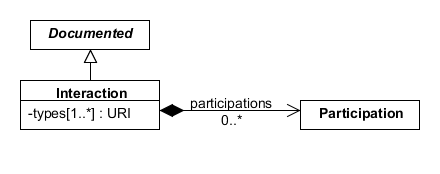
\includegraphics[scale=0.6]{uml/interaction}
\caption[]{Diagram of the \sbol{Interaction} class and its associated properties.}
\label{uml:interaction}
\end{center}
\end{figure}

The \sbol{Interaction} class provides more detailed description of how the \sbol{Feature} objects of a\\ \sbol{Component} are intended to work together.
For example, this class can be used to represent different forms of genetic regulation (e.g., transcriptional activation or repression), processes from the central dogma of biology (e.g. transcription and translation), and other basic molecular interactions (e.g., non-covalent binding or enzymatic phosphorylation).
Each \sbol{Interaction} includes a \sbolmult{types:I}{types} property that refers to descriptive ontology terms and a \sbol{participations} property that describes which \sbol{Feature} objects participate in the \sbol{Interaction}.

\subparagraph{The \sbolheading{types} property}\label{sec:types:I}

The \sbolmult{types:I}{types} property is a REQUIRED set of \sbol{URI}s that describes the behavior represented by an \sbol{Interaction}.

The \sbolmult{types:I}{types} property MUST contain one or more \sbol{URI}s that MUST identify terms from appropriate ontologies. It is RECOMMENDED that exactly one \sbol{URI} contained by the \sbolmult{types:I}{types} property refer to a term from the occurring entity branch of the Systems Biology Ontology (SBO). (See \url{http://www.ebi.ac.uk/sbo/main/}) \ref{tbl:interaction_types} provides a list of possible SBO terms for the \sbolmult{types:I}{types} property and their corresponding \sbol{URI}s.

\begin{table}[ht]
  \begin{edtable}{tabular}{ll}
    \toprule
    \textbf{Interaction Type} & \textbf{URI for SBO Term} \\
    \midrule
    Inhibition  & \url{http://identifiers.org/biomodels.sbo/SBO:0000169}\\
    Stimulation & \url{http://identifiers.org/biomodels.sbo/SBO:0000170}\\
    Biochemical Reaction & \url{http://identifiers.org/biomodels.sbo/SBO:0000176}\\
    Non-Covalent Binding & \url{http://identifiers.org/biomodels.sbo/SBO:0000177}\\
    Degradation & \url{http://identifiers.org/biomodels.sbo/SBO:0000179}\\
    Genetic Production & \url{http://identifiers.org/biomodels.sbo/SBO:0000589}\\
    Control  & \url{http://identifiers.org/biomodels.sbo/SBO:0000168} \\
    \bottomrule
  \end{edtable}
  \caption{SBO terms to specify the \sbolmult{types:I}{types} property of an \sbol{Interaction}.}
  \label{tbl:interaction_types}
\end{table}

If an \sbol{Interaction} is well described by one of the terms from \ref{tbl:interaction_types}, then its \sbolmult{types:I}{types} property MUST contain the \sbol{URI} that identifies this term. Lastly, if the \sbolmult{types:I}{types} property of an \sbol{Interaction} contains multiple
 \sbol{URI}s, then they MUST identify non-conflicting terms. For example, the SBO terms ``stimulation'' and ``inhibition'' would conflict.

\subparagraph{The \sbolheading{participations} property}\label{sec:participations}

The \sbol{participations} property is an OPTIONAL and MAY contain a set of \sbol{Participation} objects, each of which identifies the \sbolmult{roles:P}{roles} that its referenced \sbol{Feature} plays in the \sbol{Interaction}.

Even though an \sbol{Interaction} generally contains at least one \sbol{Participation}, the case of zero \sbol{Participation} objects is allowed because it is plausible that a designer might want to specify that an \sbol{Interaction} will exist, even if its \sbol{participant}s have not yet been determined.

\begin{figure}[ht]
\begin{center}
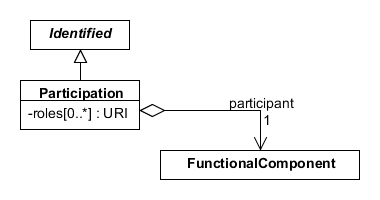
\includegraphics[scale=0.6]{uml/participation}
\caption[]{Diagram of the \sbol{Participation} class and its associated properties.}
\label{uml:participation}
\end{center}
\end{figure}

\subsubsection{Participation}
\label{sec:Participation}

Each \sbol{Participation} represents how a particular \sbol{Feature} behaves in its parent
\sbol{Interaction}.

\subparagraph{The \sbolheading{roles} property}\label{sec:roles:P}

The \sbolmult{roles:P}{roles} property is a REQUIRED set of \sbol{URI}s that describes the behavior of a \sbol{Participation} (and by extension its referenced \sbol{Feature}) in the context of its parent \sbol{Interaction}.

The \sbolmult{roles:P}{roles} property MUST contain one or more \sbol{URI}s that MUST identify terms from appropriate ontologies. It is RECOMMENDED that exactly one \sbol{URI} contained by the \sbolmult{roles:P}{roles} property refer to a term from the participant role branch of the SBO. \ref{tbl:participant_roles} provides a list of possible SBO terms for the \sbolmult{roles:P}{roles} property and their corresponding \sbol{URI}s.

\begin{table}[ht]
  \begin{edtable}{tabular}{lll}
    \toprule
    \textbf{Participation Role} & \textbf{URI for SBO Term} & \textbf{Interaction Types}\\
    \midrule
    Inhibitor  & \url{http://identifiers.org/biomodels.sbo/SBO:0000020} & Inhibition\\
    Inhibited  & \url{http://identifiers.org/biomodels.sbo/SBO:0000642} & Inhibition\\
    Stimulator & \url{http://identifiers.org/biomodels.sbo/SBO:0000459}  & Stimulation\\
    Stimulated & \url{http://identifiers.org/biomodels.sbo/SBO:0000643}  & Stimulation\\
     Reactant & \url{http://identifiers.org/biomodels.sbo/SBO:0000010}  & Non-Covalent Binding, Degradation \\
     & & Biochemical Reaction \\
    Product & \url{http://identifiers.org/biomodels.sbo/SBO:0000011}  & Non-Covalent Binding, \\
    & & Genetic Production, Biochemical Reaction\\
    Promoter  & \url{http://identifiers.org/biomodels.sbo/SBO:0000598} & Inhibition, Stimulation, Genetic Production\\
    Modifier  & \url{http://identifiers.org/biomodels.sbo/SBO:0000019} & Biochemical Reaction, Control\\
    Modified  & \url{http://identifiers.org/biomodels.sbo/SBO:0000644} & Biochemical Reaction, Control\\
    Template  & \url{http://identifiers.org/biomodels.sbo/SBO:0000645} & Genetic Production\\
%    Ligand & \url{http://identifiers.org/biomodels.sbo/SBO:0000280}\\
%    Non-Covalent Complex & \url{http://identifiers.org/biomodels.sbo/SBO:0000253}\\
    \bottomrule
  \end{edtable}
  \caption{SBO terms to specify the \sbolmult{roles:P}{roles} property of a \sbol{Participation}.}
  \label{tbl:participant_roles}
\end{table}

If a \sbol{Participation} is well described by one of the terms from \ref{tbl:participant_roles}, then its \sbolmult{roles:P}{roles} property MUST contain the \sbol{URI} that identifies this term.
Also, if a \sbol{Participation} belongs to an \sbol{Interaction} that has a type listed in \ref{tbl:interaction_types}, then the \sbol{Participation} SHOULD have a role that is cross-listed with this type in \ref{tbl:participant_roles}.
Lastly, if the \sbolmult{roles:P}{roles} property of a \sbol{Participation} contains multiple
 \sbol{URI}s, then they MUST identify non-conflicting terms. For example, the SBO terms ``stimulator'' and ``inhibitor'' would conflict.


\subparagraph{The \sbolheading{participant} property}\label{sec:participant}

The \sbol{participant} property MUST specify precisely one \sbol{Feature} object that plays the designated role in its parent \sbol{Interaction} object.


\subsubsection{Interface}
\label{sec:Interface}

\begin{figure}[ht]
\begin{center}
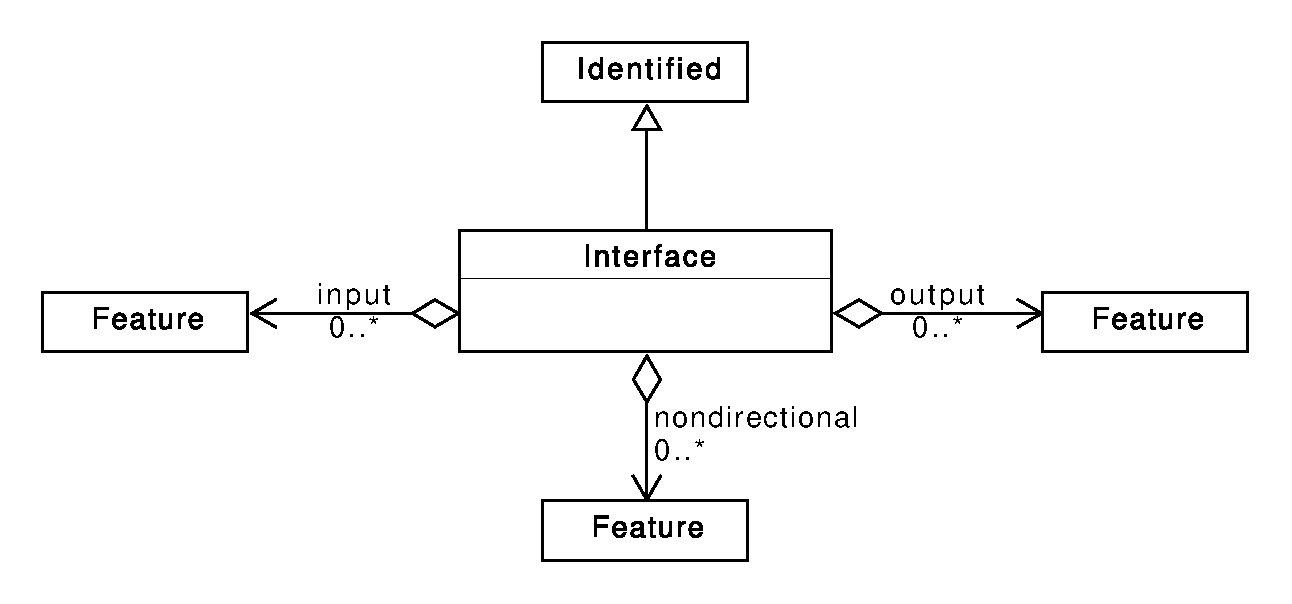
\includegraphics[scale=0.6]{uml/interface}
\caption[]{Diagram of the \sbol{Interface} class and its associated properties.}
\label{uml:interface}
\end{center}
\end{figure}

The \sbol{Interface} class is a way of explicitly specifying the interface of a \sbol{Component}. 

\subparagraph{The \sbolheading{input} property}
\label{sec:input:Interface}
The \sbolmult{input:Interface}{input} property is OPTIONAL and MAY contain a set of \sbol{Feature} \sbol{URI}s in the same \sbol{Component}.
\subparagraph{The \sbolheading{output} property}
\label{sec:output:Interface}
The \sbolmult{output:Interface}{output} property is OPTIONAL and MAY contain a set of \sbol{Feature} \sbol{URI}s in the same \sbol{Component}.

\subparagraph{The \sbolheading{nondirectional} property}
\label{sec:nondirectional:Interface}
The \sbolmult{nondirectional:Interface}{nondirectional} property is OPTIONAL and MAY contain a set of \sbol{Feature} \sbol{URI}s in the same \sbol{Component}. Note that nondirectional can imply both bidirectional as well as situations where there are no flows (for instance - a physical interface).





\subsection{CombinatorialDerivation}
\label{sec:CombinatorialDerivation}

The purpose of the \sbol{CombinatorialDerivation} class is to specify combinatorial biological designs without having to specify every possible design variant. For example, a \sbol{CombinatorialDerivation} can be used to specify a library of reporter gene variants that include different promoters and RBSs without having to specify a \sbol{Component} for every possible combination of promoter, RBS, and CDS in the library. \sbol{Component} objects that realize a \sbol{CombinatorialDerivation} can be derived in accordance with the class properties \sbol{template}, \\
\sbol{hasVariableFeature}, and \sbol{strategy} (see \ref{uml:combinatorial_derivation}).

\begin{figure}[ht]
\begin{center}
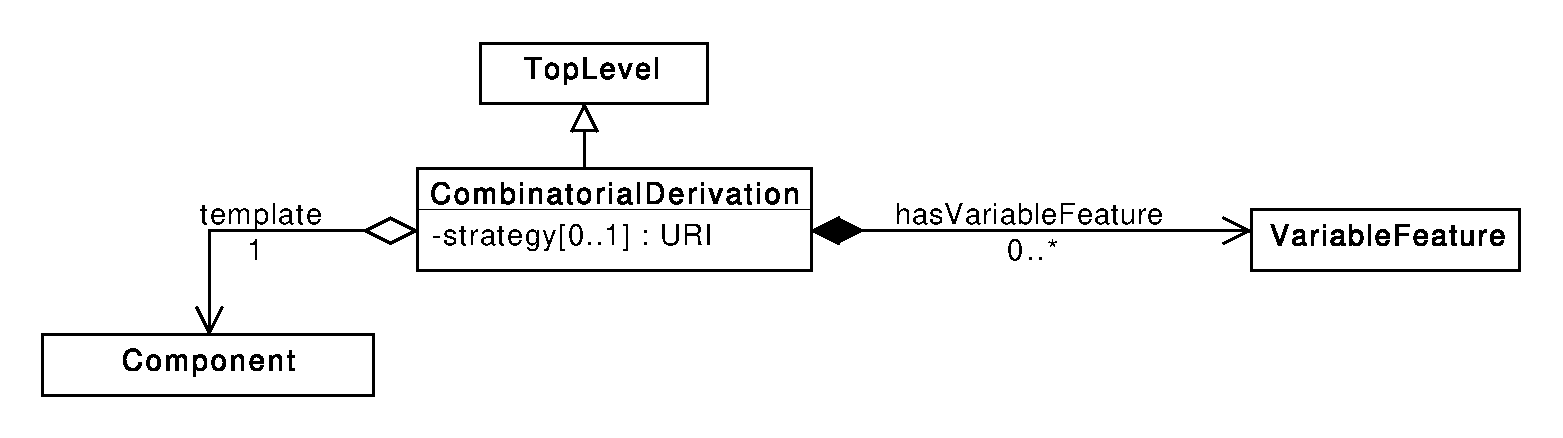
\includegraphics[scale=0.6]{uml/combinatorial_derivation}
\caption[]{Diagram of the \sbol{CombinatorialDerivation} class and its associated properties.}
\label{uml:combinatorial_derivation}
\end{center}
\end{figure}

\subparagraph{The \sbolheading{template} property}\label{sec:template}

The \sbol{template} property is REQUIRED and MUST contain a URI that refers to a \sbol{Component}. 
This \sbol{Component} is expected to serve as a template for the derivation of new \sbol{Component} objects. 
Consequently, its \sbol{hasFeature} properties SHOULD contain one or more \sbol{Feature} objects that describe its substructure (referred to hereafter as template \sbol{Feature} objects), and its other properties MAY also describe other aspects of the template that will not change based on the values that ay be varied.

When a \sbol{Component} is derived in accordance with a \sbol{CombinatorialDerivation}, the \prov{wasDerivedFrom} property of the derived \sbol{Component} SHOULD refer to the \sbol{CombinatorialDerivation}. When multiple \sbol{Component} objects are derived in accordance with the same \sbol{CombinatorialDerivation}, they MAY be referred to by the \sbol{member} property of a \sbol{Collection}, in which case the \prov{wasDerivedFrom} property of the \sbol{Collection} SHOULD also refer to this \sbol{CombinatorialDerivation}.

If the \sbolmult{type:C}{type} property of the template \sbol{Component} contains one or more URIs, then the \sbolmult{type:C}{type} property of any derived \sbol{Component} SHOULD also contain those URIs. 
The same holds true for the \sbolmult{role:C}{role} properties of these \sbol{Component} objects.

\subparagraph{The \sbolheading{hasVariableFeature} property}\label{sec:hasVariableFeature}

Each \sbol{VariableFeature} child of a \sbol{CombinatorialDerivation} defines the set of possible values for one of the variables in the \sbol{template}.
A \sbol{CombinatorialDerivation} object can have zero or more \sbol{hasVariableFeature} properties, each of type \sbol{URI}, specifying a \sbol{VariableFeature}. 
The set of  \sbol{hasVariableFeature} properties MUST NOT contain two or more \sbol{VariableFeature} objects that refer to the same template \sbol{Feature} via their \sbol{variable} properties (i.e., do not define the same variable twice).

The \sbol{variable} properties of \sbol{VariableFeature} objects control which \sbol{Feature} objects in the \sbol{template} are modified in a derived \sbol{Component}.
If no \sbol{variable} property of one of these \sbol{VariableFeature} objects refers to a template \sbol{Feature}, then it is not a variable and the derived object SHOULD have a \sbol{Feature} with identical properties
and a \prov{wasDerivedFrom} property that refers to the template \sbol{Feature}.

If a \sbol{Feature} in the \sbol{template} is referred to by some \sbol{variable} in a \sbol{VariableFeature}, then it is a variable and it SHOULD be replaced in the derived \sbol{Component} by a number of \sbol{Feature} objects constrained by the number specified by the \sbol{cardinality} property of the \sbol{VariableFeature} (see \ref{tbl:cardinality}).
Each property of such a \sbol{Feature} object in the derived \sbol{Component} MUST be derived from the values of the  associated \sbol{VariableFeature}.


Finally, all derived \sbol{Feature} objects MUST follow the \sbol{restriction} properties of any 
\sbol{Constraint} objects that refer to their corresponding template \sbol{Feature}, and SHOULD have values of \sbolmult{role:F}{role} that contain the same values as the \sbolmult{role:F}{role} in the template \sbol{Feature}.


\subparagraph{The \sbolheading{strategy} property}\label{sec:strategy}
The \sbol{strategy} property is OPTIONAL and has a data type of URI. \ref{tbl:strategy} provides a list of REQUIRED \sbol{strategy} URIs. If the \sbol{strategy} property is not empty, then it MUST contain a URI from \ref{tbl:strategy}. This property recommends how many \sbol{Component} objects SHOULD be derived from the template \sbol{Component}.

\begin{table}[ht]
  \begin{edtable}{tabular}{lp{4in}}
    \toprule
    \textbf{Strategy URI} & \textbf{Description} \\
    \midrule
    \url{http://sbols.org/v3#enumerate}  &  Derivation SHOULD produce all possible \sbol{Component} objects specified by the \sbol{CombinatorialDerivation}. \\
        \url{http://sbols.org/v3#sample}  & Derivation SHOULD produce a subset of possible \sbol{Component} objects specified by \sbol{CombinatorialDerivation}. The manner in which this subset is chosen is left unspecified. \\
    \bottomrule
  \end{edtable}
  \caption{REQUIRED \sbol{URI}s for the \sbol{strategy} property.}
  \label{tbl:strategy}
\end{table}

\subsubsection{VariableFeature}
\label{sec:VariableFeature}

As described \sbolmult{hasVariableFeature}{above}, the \sbol{VariableFeature} class specifies a variable and set of values that will replace one of the \sbol{Feature} objects in the \sbol{template} of a \sbol{CombinatorialDerivation}.
The variable is specified by the \sbol{variable} property,
and the set of values is defined by the union of \sbol{Component} objects referred to by the \sbol{variant}, \sbol{variantCollection}, and \sbol{variantDerivation} properties.

Note that this union is intended to be a set and not a multi-set.
For example, if the \sbol{variant} property contains a \sbol{Component} $A$ and the \sbol{variantCollection} property has a \sbol{Collection} containing both \sbol{Component} $A$ and  \sbol{Component} $B$, then $A$ SHOULD NOT be selected twice during enumeration, and it SHOULD NOT be selected twice as much as $B$ during sampling.

Given a set of values linked from a \sbol{VariableFeature}, it SHOULD be the case that all value are of type \sbol{om:Measure} or else all values are of type \sbol{Feature}. At present, it is explicitly left undefined how derivation of new components ought to handle mixtures of \sbol{om:Measure} and \sbol{Feature} values.

\begin{figure}[ht]
\begin{center}
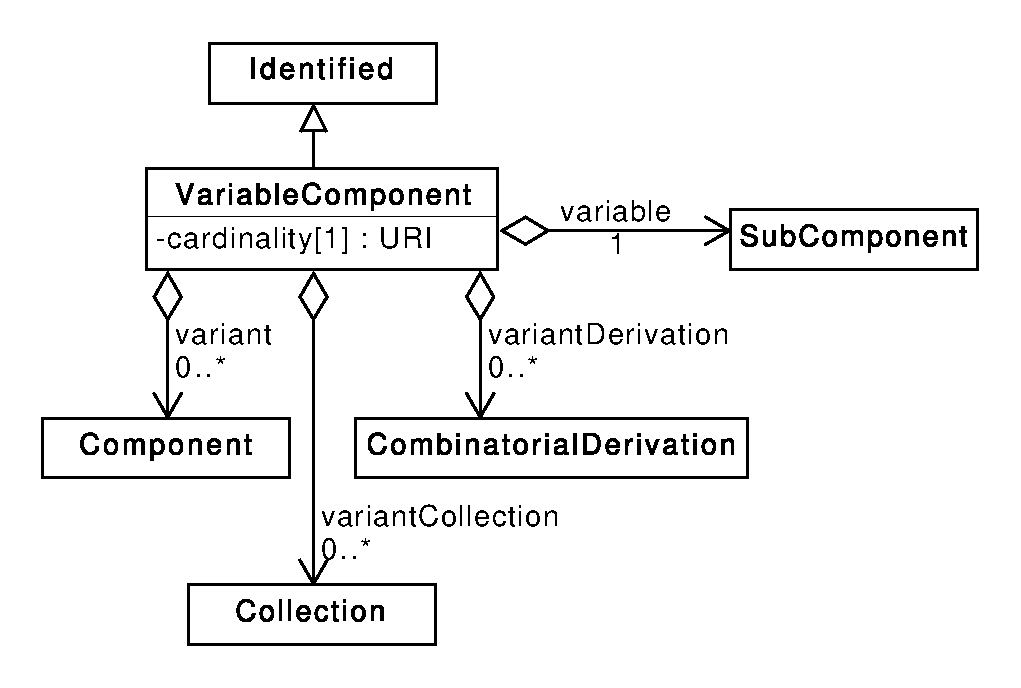
\includegraphics[scale=0.6]{uml/variable_component}
\caption[]{Diagram of the \sbol{VariableFeature} class and its associated properties.}
\label{uml:variable_component}
\end{center}
\end{figure}

\subparagraph{The \sbolheading{variable} property}\label{sec:variable}

The \sbol{variable} property is REQUIRED and MUST contain a URI that refers to a template \sbol{Feature} in the \sbol{template} \sbol{Component} referred to by this \sbol{VariableFeature}'s parent \sbol{CombinatorialDerivation}

\subparagraph{The \sbolheading{variantMeasure} property}\label{sec:variantMeasure}

A \sbol{VariableFeature} object can have zero or more \sbol{variantMeasure} properties, each of type \sbol{URI}, specifying a \sbol{om:Measure} object. This property specifies numerical values that are options to be applied to the \sbol{variable} \sbol{Feature} from the \sbol{template} when deriving a new \sbol{Component}.

Note that because a \sbol{om:Measure} is not a \sbol{TopLevel}, the vlaues of \sbol{variantMeasure} must be child objects of the \sbol{VariableFeature}.

\subparagraph{The \sbolheading{variant} property}\label{sec:variant}

A \sbol{VariableFeature} object can have zero or more \sbol{variant} properties, each of type \sbol{URI}, specifying a \sbol{Component} object. This property specifies individual \sbol{Component} objects to serve as options when deriving a new
\sbol{Feature} for the \sbol{variable} \sbol{Feature} from the \sbol{template}.

\subparagraph{The \sbolheading{variantCollection} property}\label{sec:variantCollection}

A \sbol{VariableFeature} object can have zero or more \sbol{variantCollection} properties, each of type \sbol{URI}, specifying a \sbol{Collection} object.
Such a \sbol{Collection} MUST NOT contain any objects besides \sbol{Component} objects or \sbol{Collection} objects that themselves contain only \sbol{Component} or \sbol{Collection} objects.
This property enables the specification of existing groups of \sbol{Component} objects to serve as options.

\subparagraph{The \sbolheading{variantDerivation} property}\label{sec:variantDerivation}

A \sbol{VariableFeature} object can have zero or more \sbol{variantDerivation} properties, each of type \sbol{URI}, specifying a \sbol{CombinatorialDerivation} object. 
This property enables the specification of \sbol{Component} objects derived in accordance with another \sbol{CombinatorialDerivation} to serve as options when deriving a new \sbol{Feature} for the \sbol{variable} \sbol{Feature} from the \sbol{template}. 
The \sbol{variantDerivation} properties of a \sbol{VariableFeature} MUST NOT refer to the \sbol{CombinatorialDerivation} that contains this \sbol{VariableFeature}. 
Furthermore, such \sbol{VariableFeature} objects MUST NOT form a cyclical chain of references via their \sbol{variantDerivation} properties and the \sbol{CombinatorialDerivation} objects that contain them. 

\subparagraph{The \sbolheading{cardinality} property}\label{sec:cardinality}

The \sbol{cardinality} property is REQUIRED and has type of URI. This property specifies how many \sbol{Feature} objects SHOULD be derived from the template \sbol{Feature} during the derivation of a new \sbol{Component}. The URI value of this property MUST come from the URIs provided in~\ref{tbl:cardinality}.

\begin{table}[ht]
  \begin{edtable}{tabular}{lp{4in}}
    \toprule
    \textbf{Cardinality URI} & \textbf{Description} \\
    \midrule
    \url{http://sbols.org/v3#zeroOrOne} & No more than one \sbol{Feature} in the derived \sbol{Component} SHOULD have a \prov{wasDerivedFrom} property that refers to the template \sbol{Feature}. \\
        \url{http://sbols.org/v3#one} & Exactly one \sbol{Feature} in the derived \sbol{Component} SHOULD have a \prov{wasDerivedFrom} property that refers to the template \sbol{Feature}. \\
\url{http://sbols.org/v3#zeroOrMore} & Any number of \sbol{Feature} objects in the derived \sbol{Component} MAY have \prov{wasDerivedFrom} properties that refer to the template \sbol{Feature}. \\
\url{http://sbols.org/v3#oneOrMore} & At least one \sbol{Feature} in the derived \sbol{Component} SHOULD have a \prov{wasDerivedFrom} property that refers to the template \sbol{Feature}. \\
    \bottomrule
  \end{edtable}
  \caption{REQUIRED \sbol{URI}s for the \sbol{cardinality} property.}
  \label{tbl:cardinality}
\end{table}



\subsection{Implementation}
\label{sec:Implementation}


An \sbol{Implementation} represents an instance of a synthetic biological construct, and describes the build phase of a design-built-test-learn workflow. Importantly, an \sbol{Implementation} can be associated with a laboratory sample that was already built, or that is to be built in the future. An \sbol{Implementation} can also represent virtual and simulated instances.  An \sbol{Implementation} may be linked back to its original design (i.e., a \sbol{Component}) using the \sbol{prov:wasDerivedFrom} property inherited from the \sbol{Identified} superclass. An \sbol{Implementation} may also link to a \sbol{Component} that specifies its realized structure and/or function.
% as described in Section2.1.1.

\begin{figure}[ht]
\begin{center}
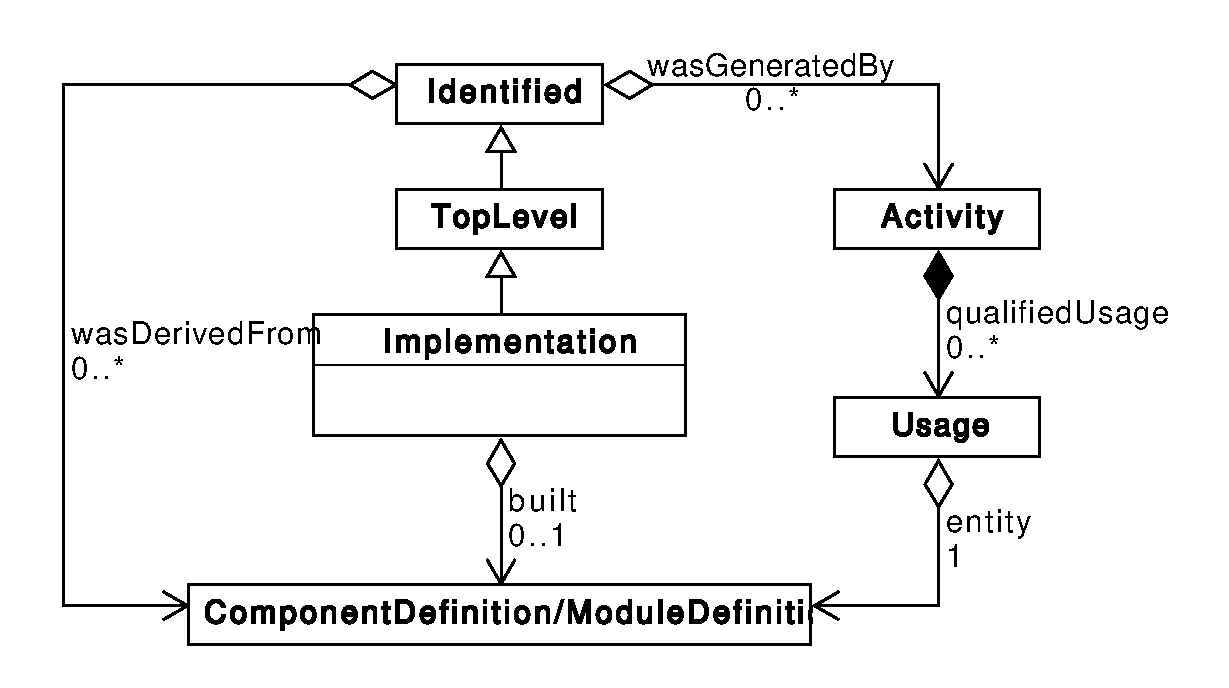
\includegraphics[scale=0.5]{uml/implementation}
\caption[]{Diagram of the \sbol{Implementation} class and its associated properties.}
\label{uml:implementation}
\end{center}
\end{figure}

\subparagraph{The \sbolheading{built} property}\label{sec:built}
The \sbol{built} property is OPTIONAL and MAY contain a URI that MUST refer to a \sbol{Component}. This \sbol{Component} is intended to describe the actual physical structure and/or functional behavior of the \sbol{Implementation}. When the built property refers to a \sbol{Component} that is also linked to the \sbol{Implementation} via PROV-O properties such as \sbol{prov:wasDerivedFrom} (see \ref{sec:provenance}), it can be inferred that the actual structure and/or function of the \sbol{Implementation} matches its original design. When the \sbol{built} property refers to a different \sbol{Component}, it can be inferred that the \sbol{Implementation} has deviated from the original design. For example, the latter could be used to document when the DNA sequencing results for an assembled construct do not match the original target sequence.





\subsection{ExperimentalData}
\label{sec:ExperimentalData}


\begin{figure}[ht]
\begin{center}
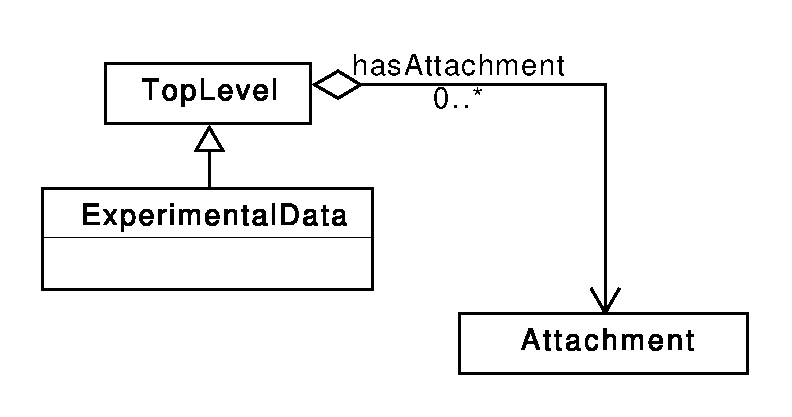
\includegraphics[scale=0.6]{uml/experimental_data}
\caption[]{Diagram of the \sbol{ExperimentalData} class and its associated properties.}
\label{uml:experimental_data}
\end{center}
\end{figure}

The purpose of the \sbol{ExperimentalData} class is to aggregate links to experimental data files. An \sbol{ExperimentalData} is typically associated with a single sample, lab instrument, or experimental condition and can be used to describe the output of the test phase of a design-build-test-learn workflow. For an example of the latter, see \ref{images:design-build-test-learn}.

As shown in \ref{uml:experimental_data}, the \sbol{ExperimentalData} class aggregates links to experimental data files using the OPTIONAL \sbol{hasAttachment} property that it inherits from the \sbol{TopLevel} class.


\subsection{Model}
\label{sec:Model}

\begin{figure}[ht]
\begin{center}
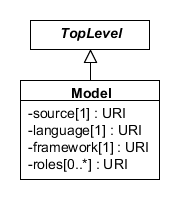
\includegraphics[scale=0.6]{uml/model}
\caption[]{Diagram of the \sbol{Model} class and its associated properties.}
\label{uml:model}
\end{center}
\end{figure}

The purpose of the \sbol{Model} class is to serve as a placeholder for an external computational model and provide additional meta-data to enable better reasoning about the contents of this model.
In this way, there is minimal duplication of standardization efforts and users of SBOL can formalize the function of a \sbol{Component} in the language of their choice.

The meta-data provided by the \sbol{Model} class include the following properties: the \sbolmult{source:M}{source} or location of the actual content of the model, the \sbol{language} in which the model is implemented, and the model's \sbol{framework}.

\subparagraph{The \sbolheading{source} property}\label{sec:source:M}
The \sbolmult{source:M}{source} property is REQUIRED and MUST contain a \sbol{URI} reference to the source file for a model.

\subparagraph{The \sbolheading{language} property}\label{sec:language}
The \sbol{language} property is REQUIRED and MUST contain a \sbol{URI} that specifies the language in which the model is implemented. It is RECOMMENDED that this \sbol{URI} refer to a term from the EMBRACE Data and Methods (EDAM) ontology. \ref{tbl:model_types} provides a list of terms from this ontology and their \sbol{URI}s. If the \sbol{language} property of a \sbol{Model} is well-described by one these terms, then it MUST contain the \sbol{URI} for this term as its value.

\begin{table}[ht]
  \begin{edtable}{tabular}{ll}
    \toprule
    \textbf{Model Language} & \textbf{URI for EDAM Term} \\
    \midrule
    SBML  & \url{http://identifiers.org/edam/format_2585}\\
    CellML		 & \url{http://identifiers.org/edam/format_3240}\\
    BioPAX    & \url{http://identifiers.org/edam/format_3156}\\
    \bottomrule
  \end{edtable}
  \caption{Terms from the EDAM ontology to specify the \sbol{language} property of a \sbol{Model}.}
  \label{tbl:model_types}
\end{table}


\subparagraph{The \sbolheading{framework} property}\label{sec:framework}
The \sbol{framework} property is REQUIRED and MUST contain a \sbol{URI} that specifies the framework in which the model is implemented.
It is RECOMMENDED this \sbol{URI} refer to a term from the modeling framework branch of the SBO when possible. A few suggested modeling frameworks and their corresponding \sbol{URI}s are shown in \ref{tbl:model_frameworks}. If the \sbol{framework} property of a \sbol{Model} is well-described by one these terms, then it MUST contain the \sbol{URI} for this term as its value.

\begin{table}[ht]
  \begin{edtable}{tabular}{ll}
    \toprule
    \textbf{Framework} & \textbf{URI for SBO Term} \\
    \midrule
    Continuous  & \url{http://identifiers.org/biomodels.sbo/SBO:0000062}\\
    Discrete & \url{http://identifiers.org/biomodels.sbo/SBO:0000063}\\
    \bottomrule
  \end{edtable}
  \caption{SBO terms to specify the \sbol{framework} property of a \sbol{Model}.}
  \label{tbl:model_frameworks}
\end{table}


\subsection {Collection}
\label{sec:Collection}
The \sbol{Collection} class is a class that groups together a set of \sbol{TopLevel} objects that have something in common.
Some examples of \sbol{Collection} objects:
\begin{itemize}
\item Results of a query to find all \sbol{Component} objects in a repository that function as promoters.
\item A set of \sbol{Component} objects representing a library of genetic logic gates.
\item A \sbol{Component} for a complex design, and all of the \sbol{Component}, \sbol{Sequence}, and \sbol{Model} objects used to provide its full specification.
\end{itemize}

\begin{figure}[ht]
\begin{center}
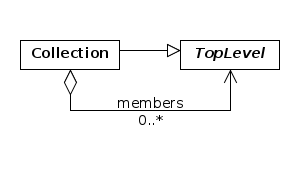
\includegraphics[scale=0.6]{uml/collection}
\caption[]{Diagram of the \sbol{Collection} class and its associated properties.}
\label{uml:collection}
\end{center}
\end{figure}

\subparagraph{The \sbolheading{member} property}\label{sec:member}
A \sbol{Collection} object can have zero or more \sbol{member} properties, each of type \sbol{URI} specifying a \sbol{TopLevel} object.

\subsubsection{Namespace}
\label{sec:Namespace}

The \sbol{Namespace} class is a subclass of \sbol{Collection} and is used to define \sbol{member} entities that share the same URI prefix.  Namely, all linked objects must have a URI prefix matching the URI of the \sbol{Namespace} object. 

\subsubsection{Experiment}
\label{sec:Experiment}

The purpose of the \sbol{Experiment} class is to aggregate \sbol{ExperimentalData} objects for subsequent analysis, usually in accordance with an experimental design.  Namely, the \sbol{member} properties of an \sbol{Experiment} MUST refer to \sbol{ExperimentalData} objects.



\subsection{Attachment}
\label{sec:Attachment}

\begin{figure}[ht]
\begin{center}
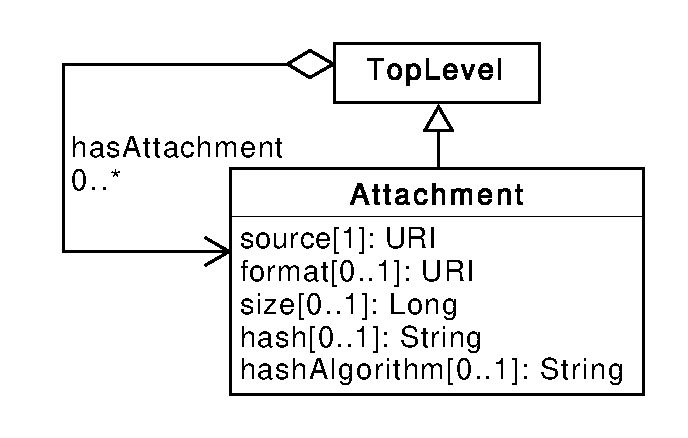
\includegraphics[scale=0.6]{uml/attachment}
\caption[]{Diagram of the \sbol{Attachment} class and its associated properties.}
\label{uml:attachment}
\end{center}
\end{figure}

The purpose of the \sbol{Attachment} class is to serve as a general container for data files, especially experimental data files.
It provides a means for linking files and metadata to SBOL designs.

The meta-data provided by the \sbol{Attachment} class include the following properties: the \sbolmult{source:A}{source} or location of the actual file of the attachment, the \sbol{format} of the file, the \sbol{size} of the file, and the \sbol{hash} for the file.

\subparagraph{The \sbolheading{source} property}\label{sec:source:A}
The \sbolmult{source:A}{source} property is REQUIRED and MUST contain a \sbol{URI} reference to the source file.

\subparagraph{The \sbolheading{format} property}\label{sec:format}
The \sbol{format} property is OPTIONAL and MAY contain a \sbol{URI} that specifies the format of the attached file. It is RECOMMENDED that this \sbol{URI} refer to a term from the EMBRACE Data and Methods (EDAM) ontology.

\subparagraph{The \sbolheading{size} property}\label{sec:size}
The \sbol{size} property is OPTIONAL and MAY contain a long indicating the file size in bytes.

\subparagraph{The \sbolheading{hash} property}\label{sec:hash}
The \sbol{hash} property is OPTIONAL and MAY contain a hash value for the file contents represented as a hexadecimal digest.

\subparagraph{The \sbolheading{hashAlgorithm} property}\label{sec:hashAlgorithm}
The \sbol{hashAlgorithm} property is OPTIONAL and MAY contain the name of the hash algorithm used to generate the value of the \sbol{hash} property.
The value of this property SHOULD be a hash name string from the \href{https://www.iana.org/assignments/named-information/named-information.xhtml}{IANA Named Information Hash Algorithm Registry}, of which \texttt{sha3-256} is currently RECOMMENDED.
If the \sbol{hash} property is set, then \sbol{hashAlgorithm} MUST be set as well.


\subsection{Annotation and Extension of SBOL}
\label{sec:Annotations}

SBOL intentionally does not attempt to describe how all types of biological design data should be captured, since many of these data types (e.g., biological context and design performance metrics) are already covered by other standards, or lack a clear consensus on their proper representation. In addition, some types of biological data are not directly relevant to design and are therefore outside of the scope of SBOL.

SBOL is built upon the Resource Description Framework (RDF), and therefore can be used in conjunction with complementary standards as described in \ref{sec:complementaryStandards}.  For example, use of the PROV-O ontology is recommended to capture provenance (see \ref{sec:provenance}).  Additionally, user-defined RDF can be used in conjunction with SBOL objects to capture custom application-specific information which does not yet have a standardized representation.  This annotation and extension mechanism is designed to enable new types of data to be easily incorporated into the SBOL standard once there is community consensus on their proper representation.

Several methods are supported for connecting the SBOL data model with other types of application-specific data:

\begin{itemize}
\item Custom data can be added to an SBOL object by annotating that object with non-conflicting properties. These properties could contain \sbol{literal} data types such as \sbol{String}s or \sbol{URI}s that require a resolution mechanism to obtain external data. An example is annotating a \sbol{Component} with  a property that contains a \sbol{String} description and \sbol{URI} for the parts registry from which its source data was originally imported.
\item Custom data in the form of independent objects can be participate in the SBOL data model if they are assigned one of the SBOL types \sbol{Identified} or \sbol{TopLevel}.  An example is an RDF object that is annotated such that it represents a data sheet that describes the performance of a \sbol{Component} in a particular context.
\item Finally, just as custom objects can be embedded in an  SBOL document, external documents can embed or refer to SBOL objects. Support for this last case is not explicitly provided in this specification. Rather, this case depends on the external non-SBOL system managing its relationship to SBOL and data serialized in RDF, and is included here for completeness.
\end{itemize}

Each \sbol{Identified} object MAY be annotated with application-specific properties, which MUST be labelled using RDF predicates outside of the SBOL namespace.  Additionally, application-specific types may be used in conjunction with the SBOL data model. These application-specific types MUST have two \sbol{rdf:type} properties: one type outside of the SBOL namespace AND an additional SBOL type of either:

\begin{itemize}
  \item \sbol{TopLevel}, if the object is to be considered an SBOL top level (i.e., not owned by another object)
  \item \sbol{Identified}, if the object is not to be considered an SBOL top level (i.e., is owned by another object)
\end{itemize}

As with SBOL \sbol{TopLevel} objects, custom \sbol{TopLevel} objects MAY include the properties \sbol{displayId}, \sbol{name},\\ \sbol{description}, etc. 


% -----------------------------------------------------------------------------
\section{Recommended Best Practices}
\label{sec:bestpractices}
% -----------------------------------------------------------------------------
\subsection{SBOL Versions}

To differentiate between major versions of SBOL, different namespaces are used.  For example, SBOL3 has the namespace \url{http://sbols.org/v3#}, while SBOL2 has the namespace \url{http://sbols.org/v2#}.  These different versions of SBOL SHOULD NOT be semantically mixed. For example, an SBOL 3.x \sbol{SubComponent} SHOULD NOT refer to an SBOL 2.x \external{ComponentInstance}, and, likewise, an SBOL 2.x \external{ComponentInstance} SHOULD NOT refer to an SBOL 1.x \external{DnaComponent}.

\subsection{Compliant SBOL Objects}
\label{sec:compliant}

Maintaining unique URIs for all SBOL objects can be challenging.  To reduce this burden, users of SBOL 3.x are encouraged to follow a few simple rules when constructing the URIs and related properties for SBOL objects.  When these rules are followed in constructing an SBOL object, we say that this object is \emph{compliant}. These rules are as follows:

Compliant URIs for \sbol{TopLevel} objects MUST conform to the following pattern:
\begin{quotation} 
\refObj{namespace}/\refObj{collection\_structure}/\refObj{displayId}
\end{quotation}

The \refObj{namespace} token MAY further decompose into \refObj{domain}/\refObj{root} tokens. The \refObj{root} and \refObj{collection\_structure} tokens may optionally be omitted; alternatively, they may consist of an arbitrary number of delimiter-separated layers. Note that this pattern means that SBOL-compliant \sbol{URI}s can be automatically decomposed with the aid of a \sbol{Namespace}. SBOL-compliant objects can be easily remapped into new namespaces by changing only the \refObj{namespace}.

Consider, for example, the SBOL-compliant \sbol{URI}:
\begin{quote}``https://synbiohub.org/igem/2017\_distribution/promoters/constitutive/BBa\_J23101''\end{quote} 
in \sbol{Namespace} ``https://synbiohub.org/igem/2017\_distribution''.
This \sbol{URI} can be decomposed as follows:
\begin{quote} 
namespace: ``https://synbiohub.org/igem/2017\_distribution'' \linebreak
domain: ``https://synbiohub.org'' \linebreak
root: ``igem/2017\_distribution'' \linebreak
collection: ``promoters/constitutive'' \linebreak
displayId: ``BBa\_J23101'' \linebreak
\end{quote}

SBOL-compliant URIs also facilitate auto-construction of child objects with unique \sbol{URI}s. 
Child objects of \sbol{TopLevel} objects with compliant \sbol{URI}s MUST conform to the following pattern:\\ ``\refObj{parent\_uri}/\refObj{child\_type}\refObj{child\_type\_counter}'' where the \refObj{parent\_uri} refers to the URI of the parent object, the \refObj{child\_type} refers to the SBOL class of the child object, and \refObj{child\_type\_counter} is a unique index for the child object. 
The \refObj{child\_type\_counter} of a new object SHOULD be calculated at time of object creation as 1 + the maximum \refObj{child\_type\_counter} for each \refObj{child\_type} object in the parent (e.g., ``\refObj{parent\_uri}/SequenceAnnotation37''). 
Note that numbering is independent for each type, so a \sbol{Component} can have children ``SubComponent37'' and ``Constraint37''.

All examples in this specification use compliant \sbol{URI}s.

\subsection{Versioning SBOL Objects}

SBOL 3.x does not specify an explicit versioning scheme. Rather it is left for experimentation across different tools. This allows version information to be included in the root (e.g., GitHub style: ``igem/HEAD/''), collection structure (e.g., ``promoters/constitutive/2/''), in tool-specific conventions on \sbol{displayId} (e.g., ``BBa\_J23101\_v2'') or in information outside of the \sbol{URI} (e.g., by attaching \external{prov:wasRevisionOf} properties).

\subsection{Annotations: Embedded Objects vs. External References}

When annotating an SBOL document with additional information, there are
two general methods that can be used:
\begin{itemize}
\item Embed the information in the SBOL document using properties outside of the SBOL namespace.
\item Store the information separately and annotate the SBOL document with \sbol{URI}s that point to it.
\end{itemize}
In theory, either method can be used in any case. (Note that a third case not
discussed here is to annotate external objects with links
to SBOL documents, rather than annotating SBOL documents with links to external objects.)

In practice, 
embedding large amounts of non-SBOL data into SBOL documents is likely
to cause problems for people and software tools trying to manage and
exchange such documents.  Therefore, it is RECOMMENDED that small amounts of information (e.g., design notes or preferred graphical layout) be embedded in the SBOL model, while large amounts of information (e.g., the contents of the scientific publication from which a model was derived or flow cytometry data that characterizes performance) be linked with URIs pointing to external resources.  The boundary between ``small'' and ``large'' is left deliberately vague, recognizing that it will likely depend on the particulars of a given SBOL application.

\subsection{Completeness and Validation}

RDF documents containing serialized SBOL objects might or might not be
entirely self-contained.  A SBOL document is self-contained or ``complete'' if every SBOL object referred to in the document is contained in the document.  It is RECOMMENDED that serializations be complete whenever practical.  In order words, when serializing an SBOL object, serialize all of the other objects that it points to, then serialize all of the other objects that these objects point to, etc., until the document is complete.

It is important to note that there is no guarantee that an RDF document
contains valid SBOL. When SBOL objects are read from an RDF document,
 the program doing so SHOULD verify that all of the property
values encoded therein have the correct data type (e.g., that the object
pointed to by the \sbol{Sequence} property of a
\sbol{Component} is really a \sbol{Sequence}).
For complete files, this validation can be carried out entirely locally. For files that are not complete, an implementation either needs to have a means of validating those external references (e.g., by
retrieving them from a repository), or it needs to mark them as
unverified and not depend on their correctness.

\subsection{Recommended Ontologies for External Terms}
\label{sec:recomm_ontologies}

External ontologies and controlled vocabularies are an integral part of SBOL. SBOL uses \sbol{URI}s to access existing biological information through these resources. 
New SBOL-specific terms are defined only when necessary. 
For example, \sbol{Component} \sbolmult{type:C}{type}s, such as DNA or protein, are described using Systems Biology Ontology (SBO) terms. Similarly, the \sbolmult{role:C}{role}s of a DNA or RNA \sbol{Component} are described via Sequence Ontology (SO) terms. Although RECOMMENDED ontologies have been indicated in relevant sections where possible, other resources providing similar terms can also be used. A summary of these external sources can be found in \ref{tbl:preferred_external_resources}.

\begin{table}[htp]
  \begin{edtable}{tabular}{p{2cm}p{1.5cm}p{5cm}p{6cm}}
    \toprule
    \textbf{SBOL Entity} & \textbf{Property} & \textbf{Preferred External Resource}
    & \textbf{More Information} \\
    \midrule
    \textbf{Component}  & type & SBO (physical entity branch)& \url{http://www.ebi.ac.uk/sbo/main/}\\
                                  & type & SO (nucleic acid topology)& \url{http://www.sequenceontology.org}\\
    						   	  & role & SO (\textit{DNA} or \textit{RNA}) & \url{http://www.sequenceontology.org}   \\
    						   	  & role & CHEBI (\textit{small molecule}) & \url{https://www.ebi.ac.uk/chebi/}   \\
							  & role & PubChem (\textit{small molecule}) & \url{https://pubchem.ncbi.nlm.nih.gov/} \\
    						   	  & role & UniProt (\textit{protein}) & \url{https://www.uniprot.org/}  \\   
    						   	  & role & NCIT (\textit{samples}) & \url{https://ncithesaurus.nci.nih.gov/}  \\   
    \textbf{Interaction}	      & type & SBO (occurring entity branch) & 
    \url{http://www.ebi.ac.uk/sbo/main/} \\
    \textbf{Participation}	      & role & SBO (participant roles branch) &
    \url{http://www.ebi.ac.uk/sbo/main/} \\
    \textbf{Model}	      		  & language & EDAM & \url{http://bioportal.bioontology.org/ontologies/EDAM}     \\
    				      		  & framework & SBO (modeling framework branch) &
    \url{http://www.ebi.ac.uk/sbo/main/} \\
    \textbf{om:Measure}	& type & SBO (systems description parameters) &
    \url{http://www.ebi.ac.uk/sbo/main/} \\
    \bottomrule
  \end{edtable}
  \caption{Preferred external resources from which to draw values for various SBOL properties.}
  \label{tbl:preferred_external_resources}
\end{table}

The URIs for ontological terms SHOULD come from identifiers.org.  However, it is acceptable to use terms from purl.org as an alternative, for example when RDF tooling requires URIs to be represented as compliant QNames.  SBOL software may convert between these forms as required.

\subsection{Annotating Entities with Date \& Time}\label{sec:DateTime}

Entities in an SBOL document can be annotated with creation and modification dates. It is RECOMMENDED that predicates, or properties, from DCMI Metadata Terms SHOULD be used to include date and time information. The \texttt{created} and \texttt{modified} terms SHOULD respectively be used to annotate SBOL entities with creation and modification dates. Date and time values SHOULD be expressed using the XML Schema \texttt{DateTime} datatype~\citep{Biron2004}. For example, ``\texttt{2016-03-16T20:12:00Z}'' specifies that the day is 16 March 2016 and the time is 20:12pm in UTC (Coordinated Universal Time).

\subsection{Annotating Entities with Authorship information}\label{sec:Authorship}

Authorship information should ideally be added to \sbol{TopLevel} entities where possible. It is RECOMMENDED that the \texttt{creator} DCMI Metadata term SHOULD be used to annotate SBOL entities with authorship information using free text. This property can be repeated for each author.
%The example below shows the use of this property for two authors and the values shown are free text \texttt{String} literals.

\subsection{Host Context / Ontologies for Experiments}

\subsubsection{Mixtures via Components}

Any \sbol{Component} can be interpreted as specifying a mixture of the material entity (SBO:0000240) \sbol{Feature}s that it includes.  The amount of each such instance included in the mixture SHOULD be specified by attaching a \om{Measure} with a \sbolmult{type:Measure}{type} set to the appropriate SBO term. The SBO terms that are RECOMMENDED as appropriate are members of the Systems Description Parameter (SBO:0000545) branch of SBO. Examples include:
\begin{itemize}
\item SBO:0000540: fraction of an entity pool (e.g., 1/3 CHO cells, 2/3 HEK cells)
\item SBO:0000472: molar concentration of an entity (e.g., 1 mM Arabinose)
\item SBO:0000361: amount of an entity pool (e.g., 200 uL M9 media)
\end{itemize}

Mixtures MAY be defined recursively, as mixtures of mixtures of mixtures, etc.

\subsubsection{Media, Inducers, and Other Reagents}

Each reagent, whether ``atomic'' (e.g., rainbow bead control) or mixture (e.g., M9 media), SHOULD be represented as a \sbol{Component}.

The roles of reagents may vary in context: for example, Arabinose may serve as an inducer or as a media carbon source. As such, role SHOULD be indicated by an NCI Thesaurus (NCIT) term in a \sbolmult{role:F}{role} property of the \sbol{SubComponent}. Examples include:
\begin{itemize}
\item NCIT:C64356: Positive Control
\item NCIT:C48694: Cell
\item NCIT:C85504: Media
\item NCIT:C14419: Strain
\item NCIT:C120268: Inducer
\end{itemize}

For more information on representing cells, strains, plasmids, and genomes, see \ref{bp:cells}

%\todo[inline]{Should we switch the GO term recommendation below to match the NCIT recommendation below?}

\subsubsection{Samples}

A complete specification of a sample SHOULD be a \sbol{Component} that includes at least:
\begin{itemize}
\item A \sbol{SubComponent} instantiating each strain in the sample
\item A \sbol{SubComponent} for the media or buffer
\item A \sbol{SubComponent} for each additional reagent added to the media (e.g., inducers, antibiotics)
\item \om{Measure}s on each of these specifying the amount in the sample
\item \om{Measure}s on the \sbol{Component} for each environmental parameter (e.g., temperature, pH, culturing time)
\end{itemize}

\subsubsection{Other Experimental Parameters}

In order to deal with parameters associated with the context in general but not specific instances, e.g., temperature, pH, total sample volume, the \sbol{hasMeasure} property of \sbol{Identified} can be used.  The \sbol{hasMeasure} of a \sbol{Component} provides context-free information (e.g., the pH of M9 media, the GC-content of a GFP coding sequence), while the \sbol{hasMeasure} of a material entity (SBO:0000240) \sbol{Feature} provides a measurement in context (e.g., the dosage of Arabinose in a sample).

Values of these parameters SHOULD be specified by attaching a \om{Measure} with a \sbolmult{type:Measure}{type} set to the appropriate SBO term. The SBO terms that are RECOMMENDED as appropriate are members of the Systems Description Parameter (SBO:0000545) branch of SBO. Examples include:
\begin{itemize}
\item SBO:0000147: thermodynamic temperature (e.g., culturing at 27 C)
\item SBO:0000332: half-life of an exponential decay (e.g., decay rate of a gRNA)
\item SBO:0000304: pH (e.g., pH of M9 media)
\end{itemize}


\subsection{Multicellular System Designs}

SBOL has been used extensively to represent designs in homogeneous systems, where the same design is implemented in every cell. However, in recent years there has been increasing interest in multicellular systems, where biological designs are split across multiple cells to optimize the system behavior and function. Therefore, there is a need to define a set of best practices so that multicellular systems can be captured using SBOL in a standard way.

\subsubsection{Representing Cell Types}
\label{bp:cells}

To represent multicellular systems using SBOL, it is first necessary to represent cells. 
When doing so, it is important to be able to capture the following information: (i) taxonomy of the strain used, (ii) interactions occurring within cells of this type, and (iii) components inside the type of cell (e.g. genomes, plasmids). 
The approach RECOMMENDED in this section is capable of capturing this information, as shown in the example in \ref{uml:cell_representation}. 
It uses a \sbol{Component} to represent a system that contains cells of the given type.
The cells themselves are represented by a \sbol{SubComponent} inside the \sbol{Component}, which is an \sbol{instanceOf} 
a \sbol{Component} capturing information about the species and strain of the cell in the design. 
This \sbol{Component} has a \sbolmult{type:C}{type} of ``cell'' from the Gene Ontology (GO:0005623), and a \sbolmult{role:C}{role} of ``physical compartment'' (SBO:0000290).
%\todo[inline]{What property are we actually recommending to use for the annotation?}
Taxonomic information is captured by annotating the class instance with a URI for an entry in the NCBI Taxonomy Database. 

As usual, other entities besides the cell that are relevant to the design are also captured as \sbol{Feature}s.
When these are contained within the cell, they are captured using a \sbol{Constraint} with restriction \texttt{contains} with the cell as \sbol{subject} and contained object as \sbol{object}.
Interactions which occur in this system are captured using the \sbol{Interaction} and \sbol{Participation} classes. 
Interactions which occur within the cell are specified by \sbol{Interaction} classes which contain the \sbol{SubComponent} instance representing the cell as a \sbol{participant} with a \sbolmult{role:P}{role} of ``physical compartment'' (SBO:0000290).

\begin{figure}[htp]
	\begin{center}
		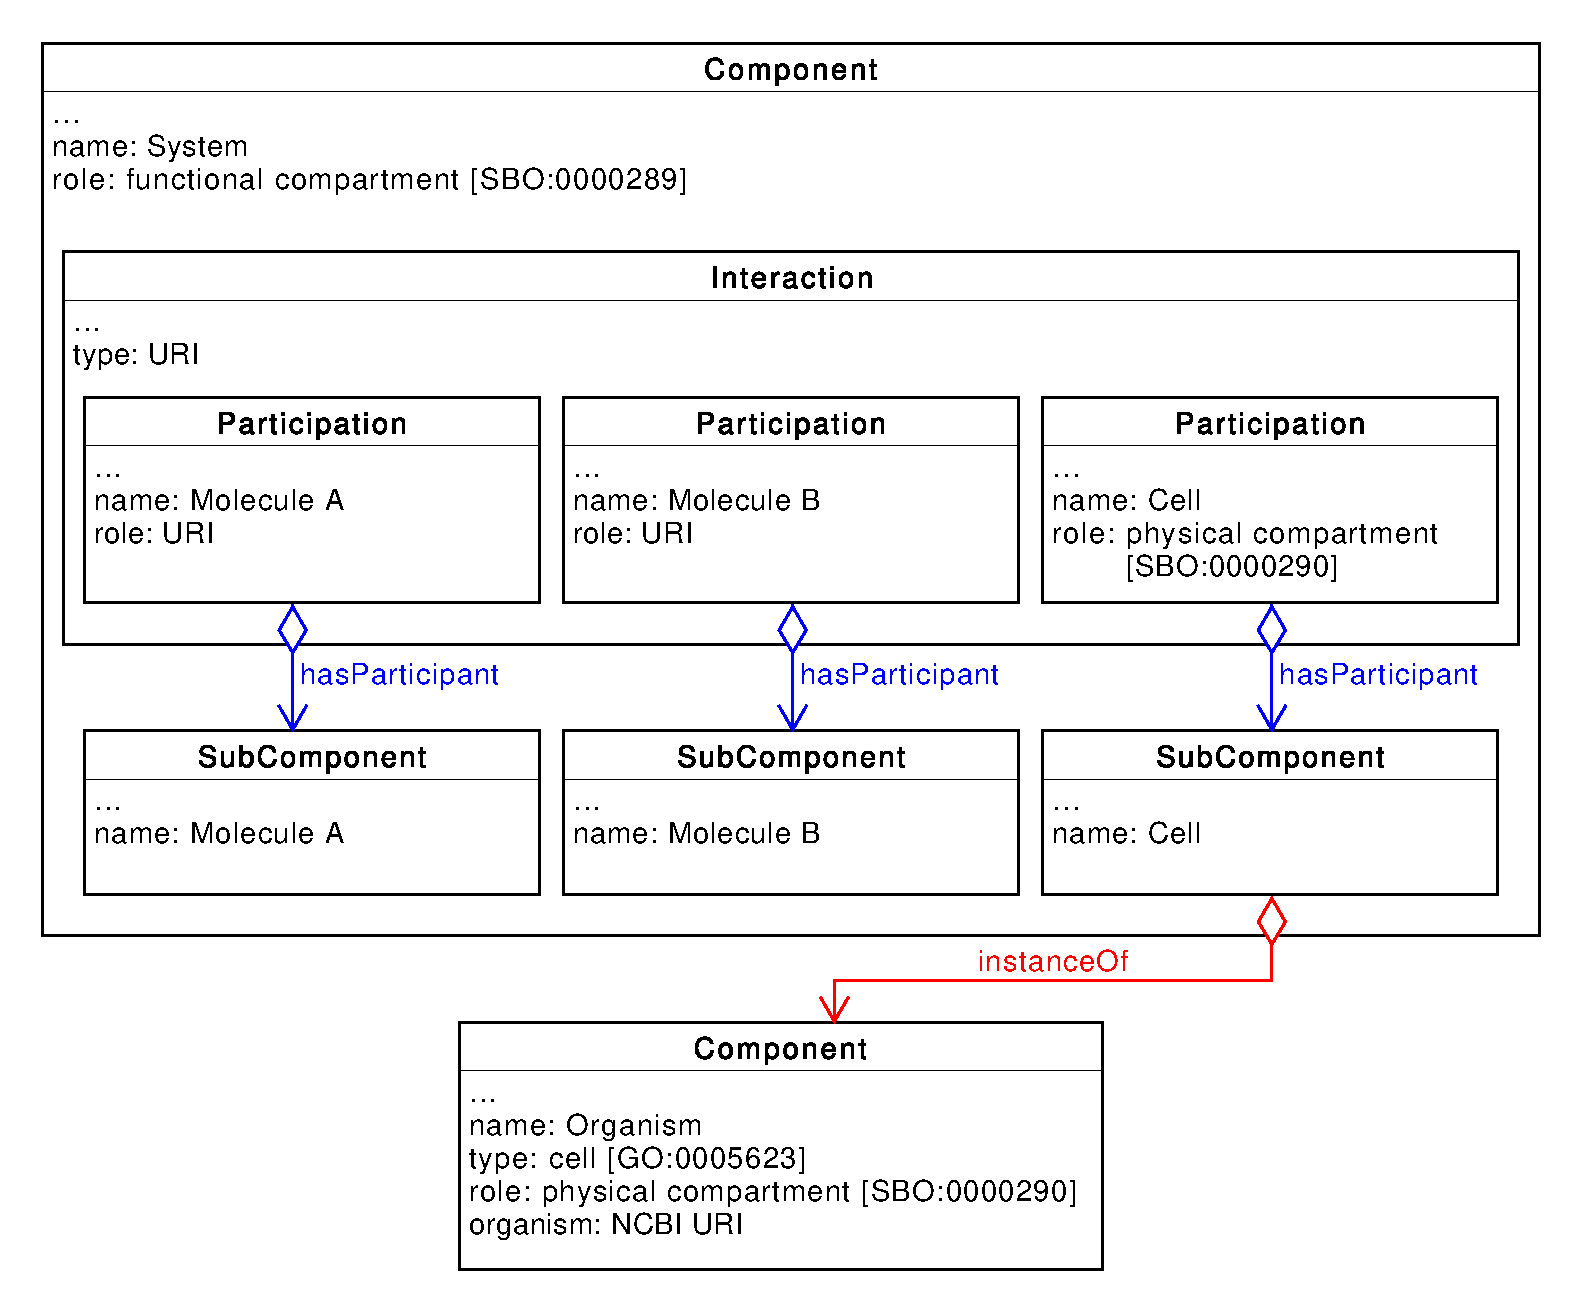
\includegraphics[width=\textwidth]{uml/cell_representation}
		\caption[Repressenting a cell]{This is a proposed approach for capturing cell designs in SBOL. A \sbol{Component} annotated with a URI pointing to an entry in the NCBI Taxonomy Database is used to capture information about the cell's strain/species. 
		The \sbol{Component} has a type of ``Cell'' from the Gene Ontology (GO), and a role of ``physical compartment''. 
		Another \sbol{Component} is used to represent a system in which the cell is implemented. 
		Entities, including the cell, are instantiated as \sbol{SubComponent}s, and processes are captured using the \sbol{Interaction} class.
		Processes that are contained within the cell are represented by including the cell as a participant with a role of ``physical compartment''. }
		\label{uml:cell_representation}
	\end{center}
\end{figure}

\subsubsection{Multiple Cell Types in a Single Design}

The same approach can be extended to represent systems with multiple types of cells.
The multicellular system can be represented as a \sbol{Component} that includes each strain of cell as a \sbol{SubComponent} that is an \sbol{instanceOf} a \sbol{Component} defining its strain.
Interactions and constraints, such as a molecule that both strains interact with, are implemented using \sbol{ComponentReference}s to link to the definitions within each cell system description.
An example is shown in \ref{uml:multiple_cell_representation}.

\begin{figure}[htp]
	\begin{center}
		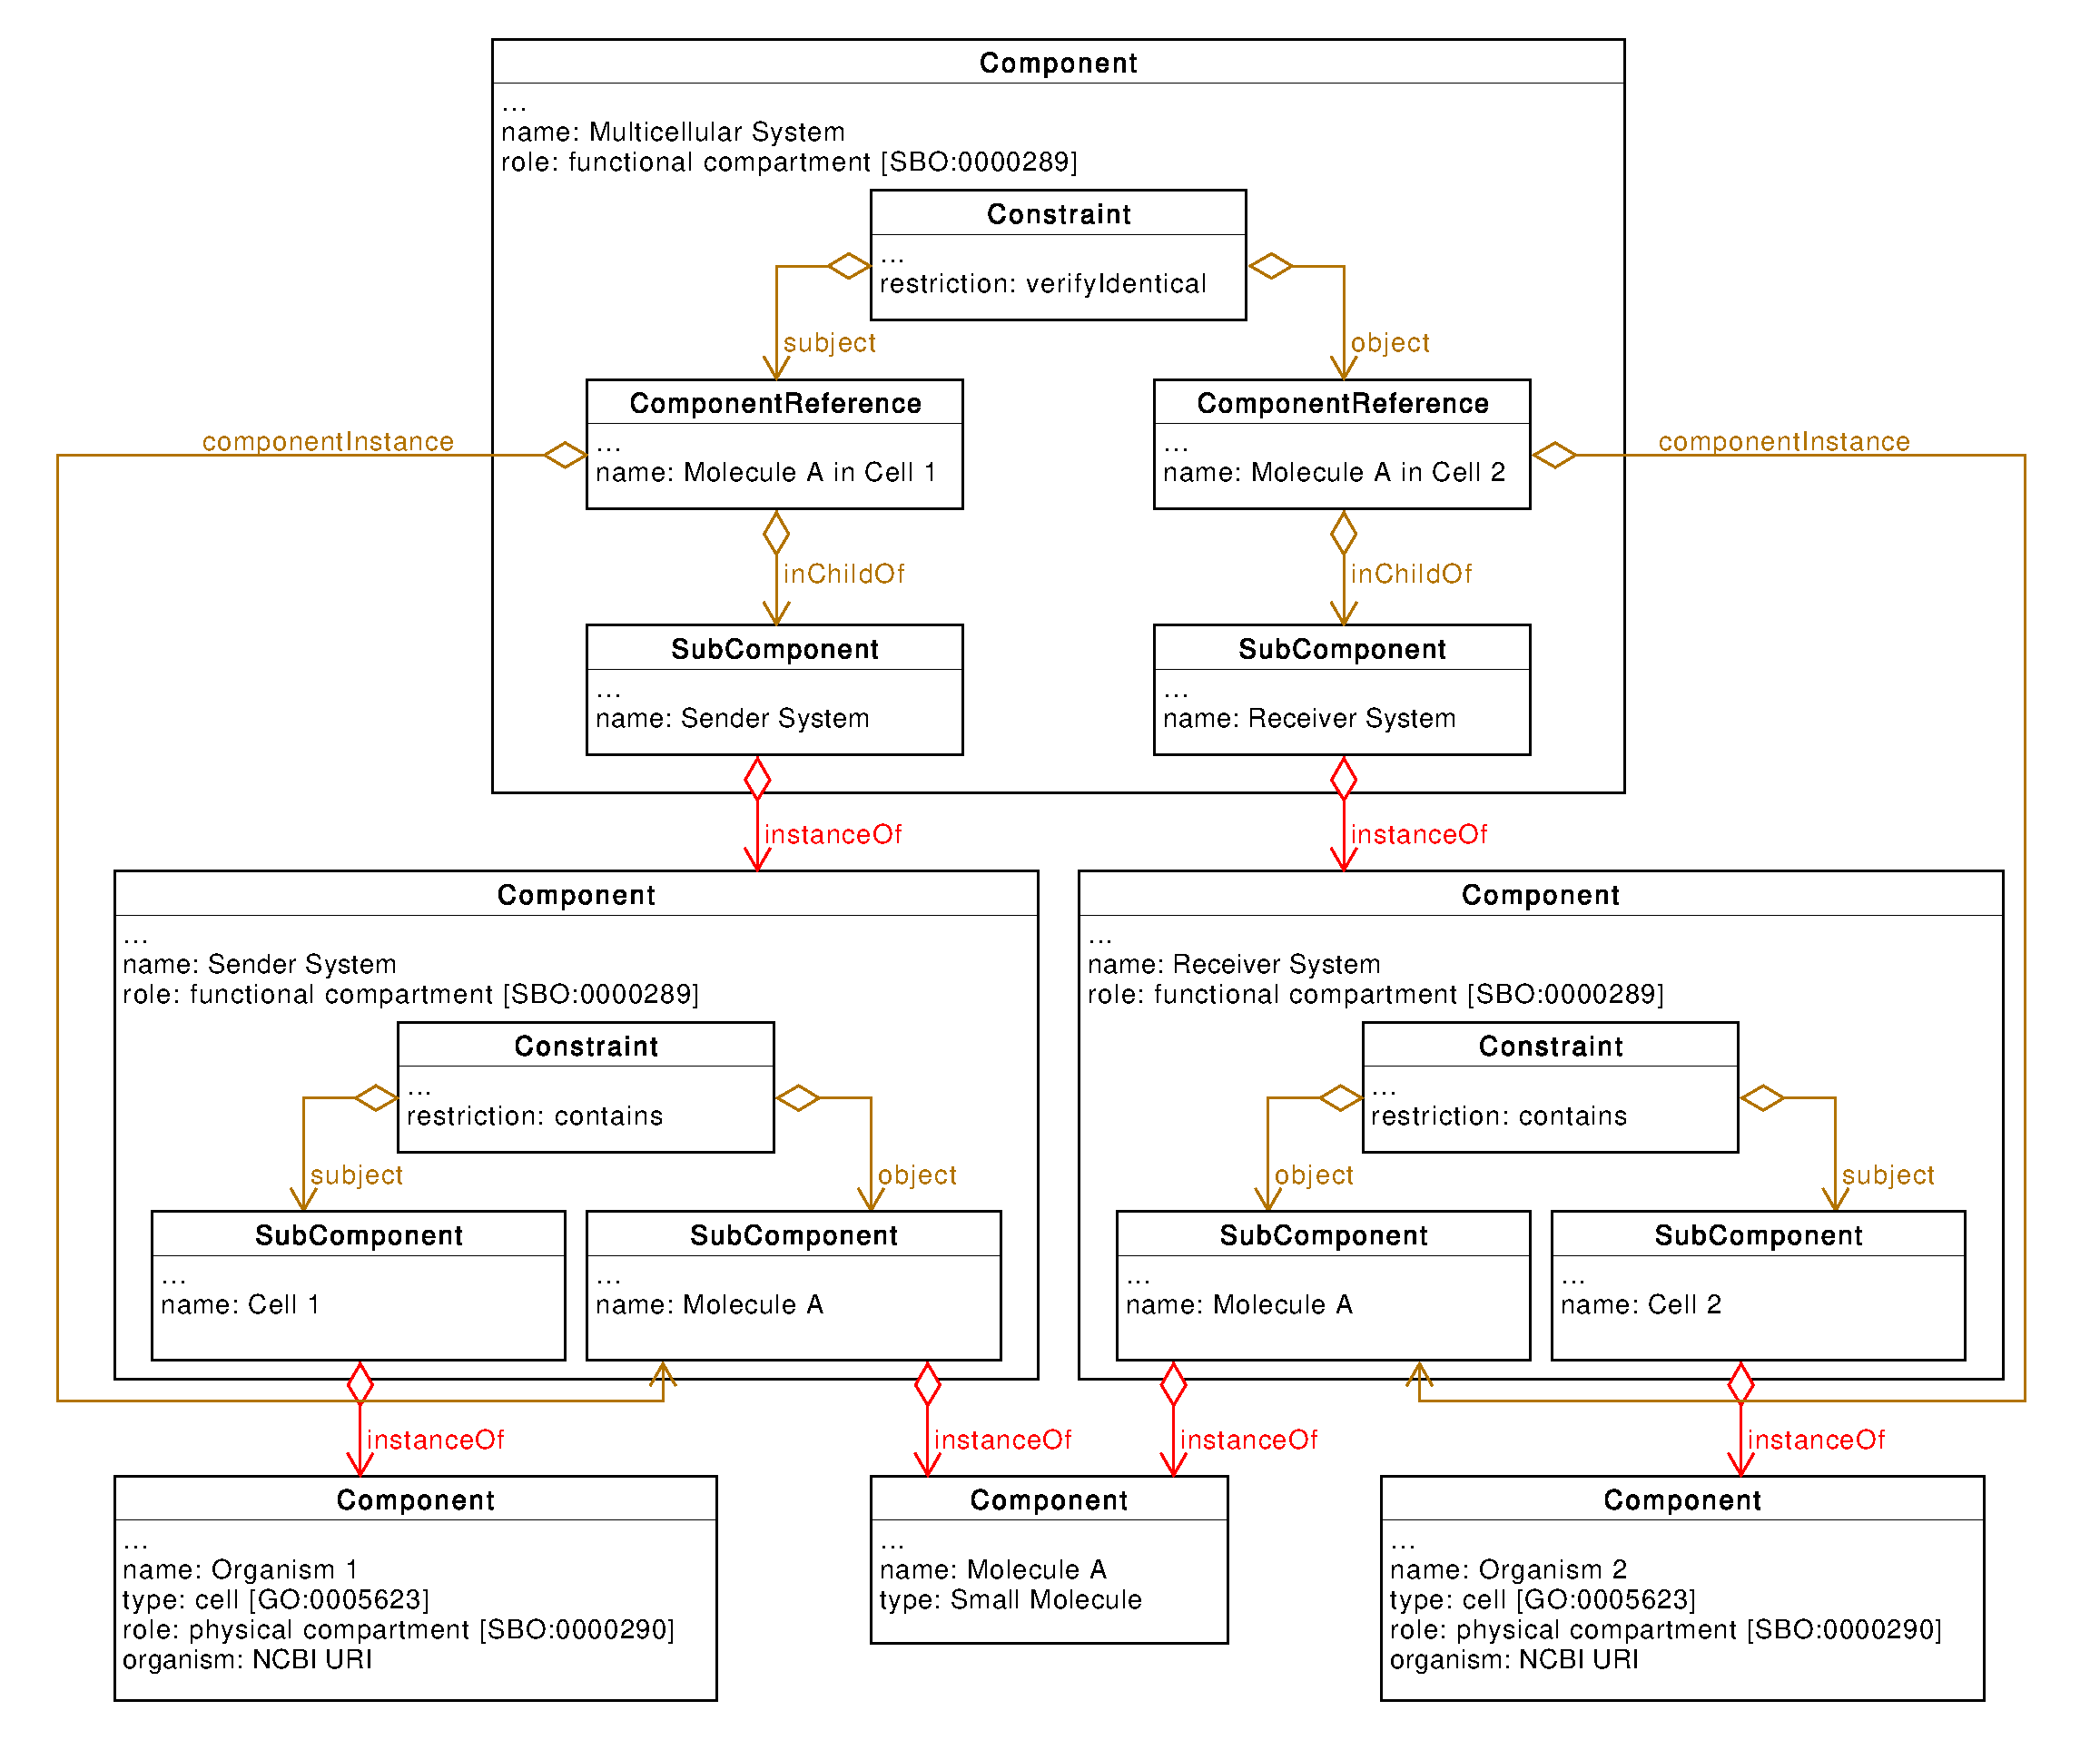
\includegraphics[width=\textwidth]{uml/two_cell_representation}
		\caption[]{Captured here is a design involving two cells which both interact with the small molecule ``Molecule A''. 
		Designs for the sender and receiver systems are captured using constraint to show that each of these cells interacts with the Molecule A contained within it.
		The overall multicellular system is represented by a \sbol{Component} with a \sbolmult{role:C}{role} of ``functional compartment'', which is an SBO term.
		The two systems are included in this multicellular design as \sbol{SubComponent}s, and the fact that Molecule A is shared between systems is indicated with a constraint.}
		\label{uml:multiple_cell_representation}
	\end{center}
\end{figure}

\subsubsection{Cell Ratios}

The proportion of cell types present in a multicellular system can be captured using \om{Measure} on the representations of cells in the design.
As a best practice, the value of these measure classes is a percentage less than or equal to 100\%, representing the amount of a cell type present in the system compared to all other cell types present. 
Therefore, the sum of all these values specified in the system will typically be equal to 100\%, though this may not be the case if the system is not completely defined. 
An example is shown in \ref{uml:cell_ratios}.

\begin{figure}[htp]
	\begin{center}
		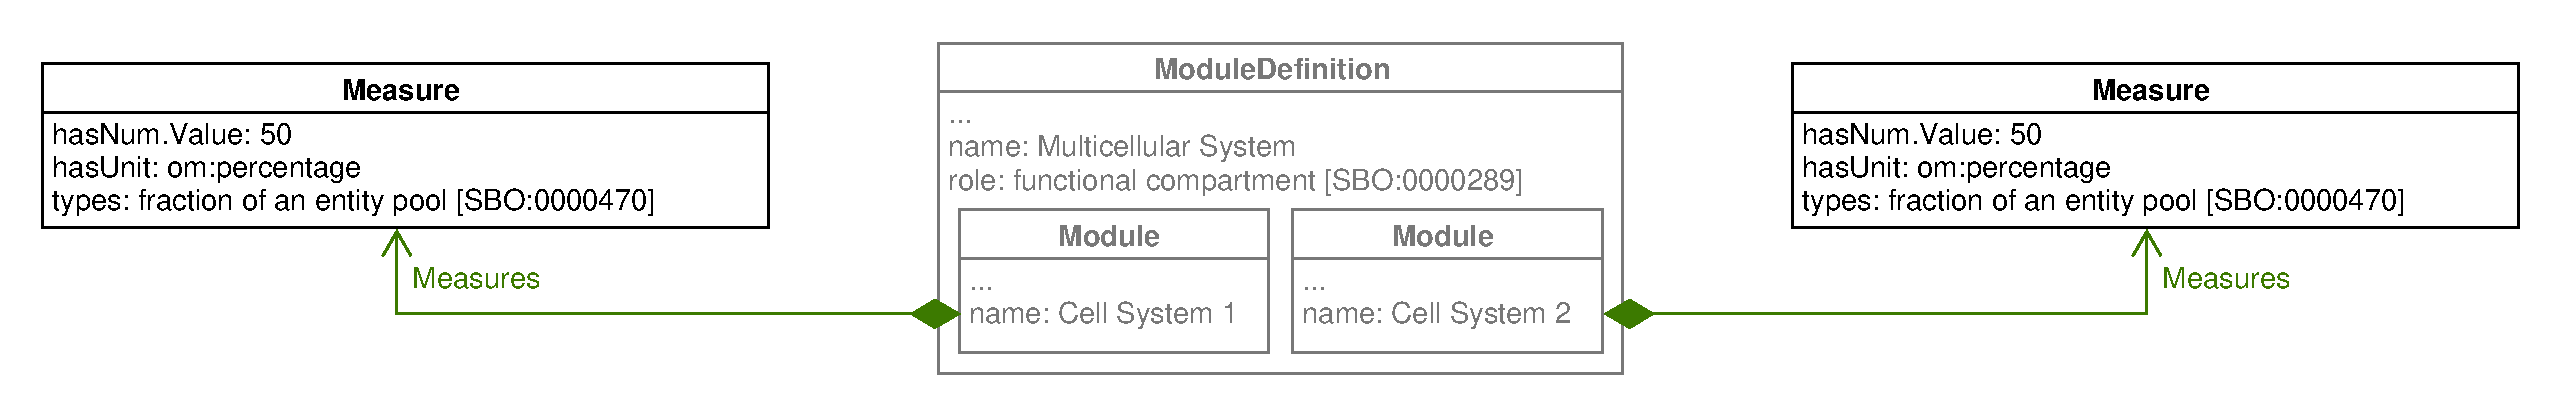
\includegraphics[width=\textwidth]{uml/cell_ratios}
		\caption[]{Annotating class instances with cellular proportions. Instances of the Measure class are used to capture the percentage of each cell type present in the multicellular system design.
		}
		\label{uml:cell_ratios}
	\end{center}
\end{figure}


% % -----------------------------------------------------------------------------
\section{Data Model Examples}
\label{sec:examples}
% -----------------------------------------------------------------------------

%\subsection{LacI/TetR Toggle Switch}

This section illustrates how to use the SBOL data model by specifying the design of a LacI/TetR toggle switch similar to those constructed in \cite{Gardner2000}. This design is visualized conceptually in \ref{images:toggle} and in detail in \ref{images:toggleswitch_modular}. 

Conceptually, the toggle switch is constructed from two mutually repressing genes.  
With repressors LacI and TetR, this results in a bi-stable system that will tend to settle into a state where precisely one of the two repressors is strongly expressed, repressing the other.
Each of these repressors can have its activity disrupted by a small molecule (IPTG for LacI, aTc for TetR), which allows the system to be ``toggled'' from one state to the other by dosing it with the appropriate small molecule.

\begin{figure}[ht]
\begin{center}
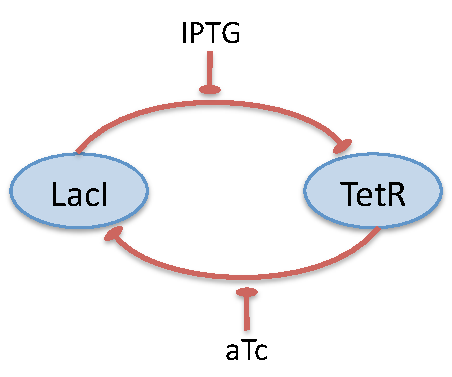
\includegraphics[scale=1.0]{images/toggle-highlevel.pdf}
\caption[]{Conceptual diagram of LacI/TetR toggle switch: the LacI 
  and TetR transcriptional factors are arranged to mutually repress, 
  creating a bi-stable system.  Transition between the two states
  is triggered by the small-molecule signals aTc (which disrupts TetR
  repression) and IPTG (which disrupts LacI repression).}
\label{images:toggle}
\end{center}
\end{figure}

\begin{figure}[ht]
\begin{center}
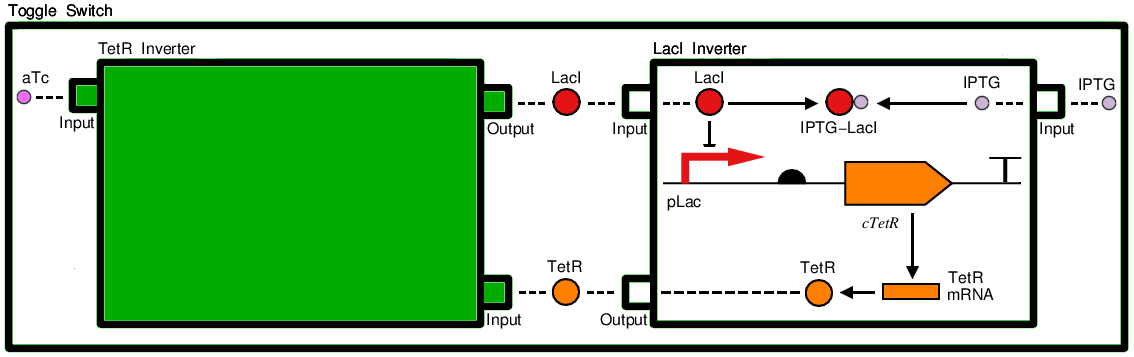
\includegraphics[scale=0.4]{images/toggleswitch_modular}
\caption[]{Design of a LacI/TetR toggle switch. This design is composed of two inverter sub-designs, each containing a single gene. These genes mutually repress each other's expression via their encoded protein transcription factors, LacI and TetR. Furthermore, both LacI and TetR are bound by specific small molecules that sequester them and prevent them from acting as repressors. In this design, arrows represent different molecular interactions, including the repression of pLac via LacI, the non-covalent binding of IPTG to LacI, the transcription of TetR mRNA, and the translation of TetR. Dashed lines serve to map between transcription factors in the inverter sub-designs and those in the overall toggle switch design.}
\label{images:toggleswitch_modular}
\end{center}
\end{figure}

The LacI/TetR toggle switch is modeled in SBOL as two parallel hierarchies of structure and function. The structural hierarchy of the toggle switch is represented using \sbol{ComponentDefinition}s:
\begin{itemize}
\item The base elements of the hierarchy are DNA components, transcription factor proteins, and small molecules. As an example, \ref{uml:ex_comp_defs} is a UML diagram of the \sbol{ComponentDefinition}s that represent these elements.
\item Base elements are composed to form more complex structures at the top of the hierarchy, including genes and non-covalent complexes between transcription factor proteins and small molecules. As an example, \ref{uml:ex_comp_def_compo} is a UML diagram of the composite \sbol{ComponentDefinition}s that represent the TetR gene and IPTG-LacI complex.
\end{itemize}

\begin{figure}[ht]
\begin{center}
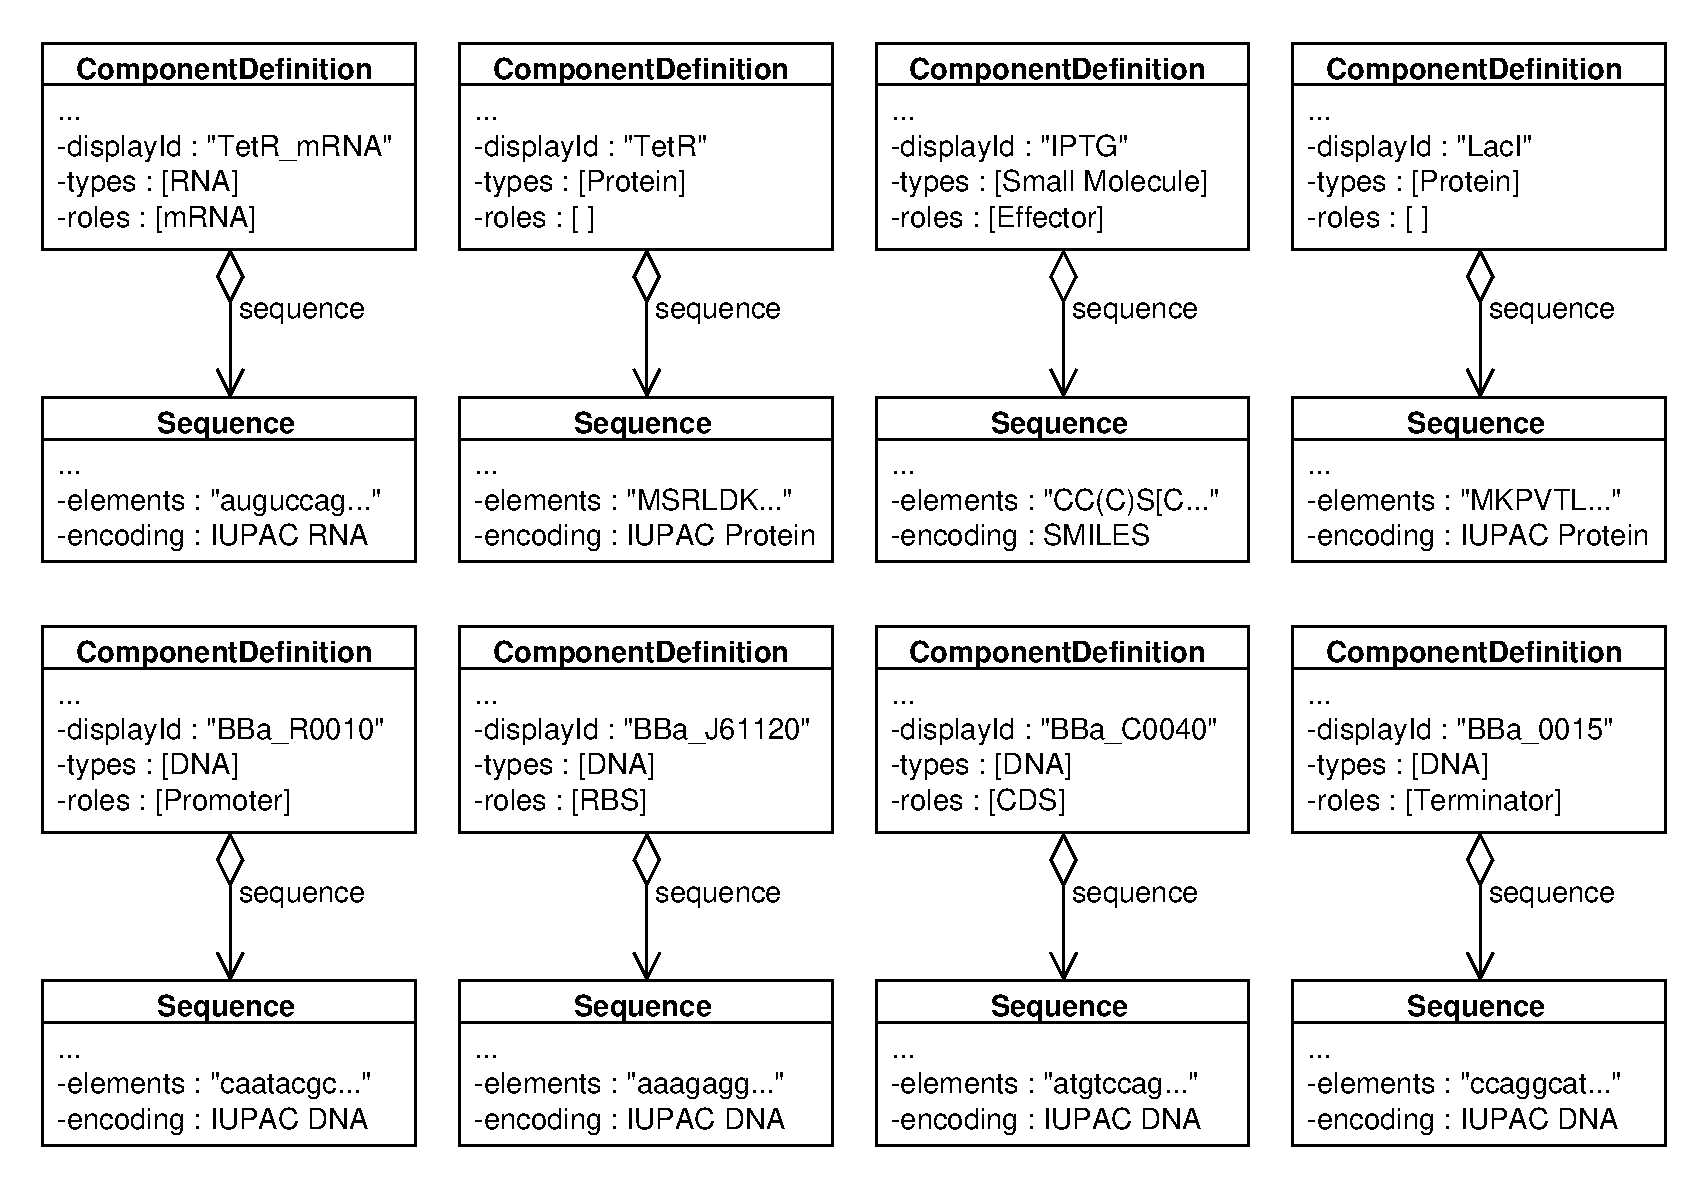
\includegraphics[width=\textwidth]{example_uml/toggle_1}
\caption[]{\sbol{ComponentDefinition} objects for the LacI inverter. These include \sbol{ComponentDefinition} objects based on DNA parts from the iGEM Registry and  \sbol{ComponentDefinition}s that represent TetR mRNA, TetR, LacI, and and IPTG. Each \sbol{ComponentDefinition} is associated with a \sbol{Sequence} that has an \external{IUPAC DNA/RNA} or \external{IUPAC protein} \sbol{encoding}, except the \sbol{ComponentDefinition} of IPTG, which is associated with a \sbol{Sequence} that has a \external{SMILES} \sbol{encoding}.}
\label{uml:ex_comp_defs}
\end{center}
\end{figure}

\begin{figure}[ht]
\begin{center}
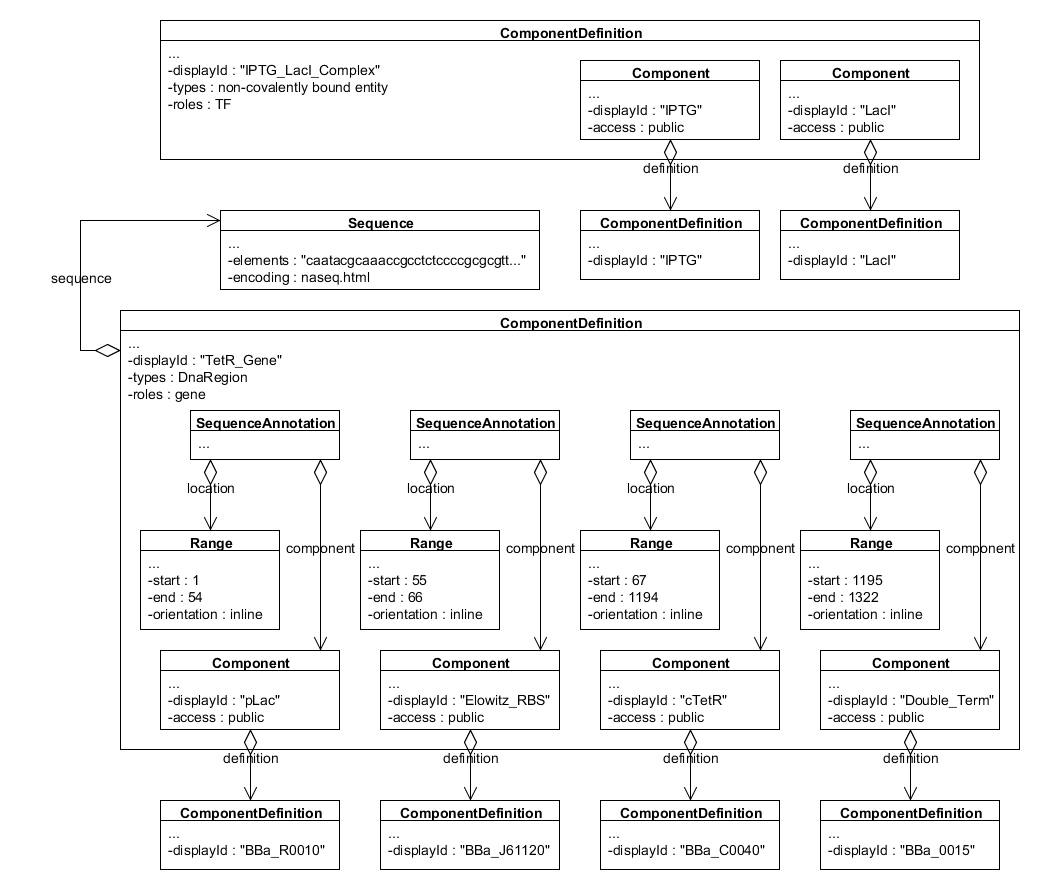
\includegraphics[width=\textwidth]{example_uml/toggle_2}
\caption[]{Composite \sbol{ComponentDefinition} objects for the LacI inverter. In the case of the \sbol{ComponentDefinition} that represents the TetR gene, its sub-\sbol{Component} objects are located as \sbol{Range}s along its \sbol{Sequence} using \sbol{SequenceAnnotation}s. The \sbol{ComponentDefinition} that represents the IPTG-LacI complex, however, has no \sbol{Sequence} and its sub-\sbol{Component} objects are composed without any data about their relative positions.}
\label{uml:ex_comp_def_compo}
\end{center}
\end{figure}

The functional hierarchy of the toggle switch is represented using
\sbol{ModuleDefinition}s:
\begin{itemize}
\item The base elements of the hierarchy are LacI-dependent repression of TetR expression (the LacI inverter) and TetR-dependent repression of LacI (the TetR inverter). As an example, \ref{uml:ex_mod_def} is a UML diagram of the \sbol{ModuleDefinition} that represents the LacI inverter.
\item Base elements are composed to form the toggle switch at the top of the hierarchy.  As an example, \ref{uml:ex_mod_def_compo} is a UML diagram of the \sbol{ModuleDefinition} that represents the toggle switch.
\end{itemize}

\begin{figure}[ht]
\begin{center}
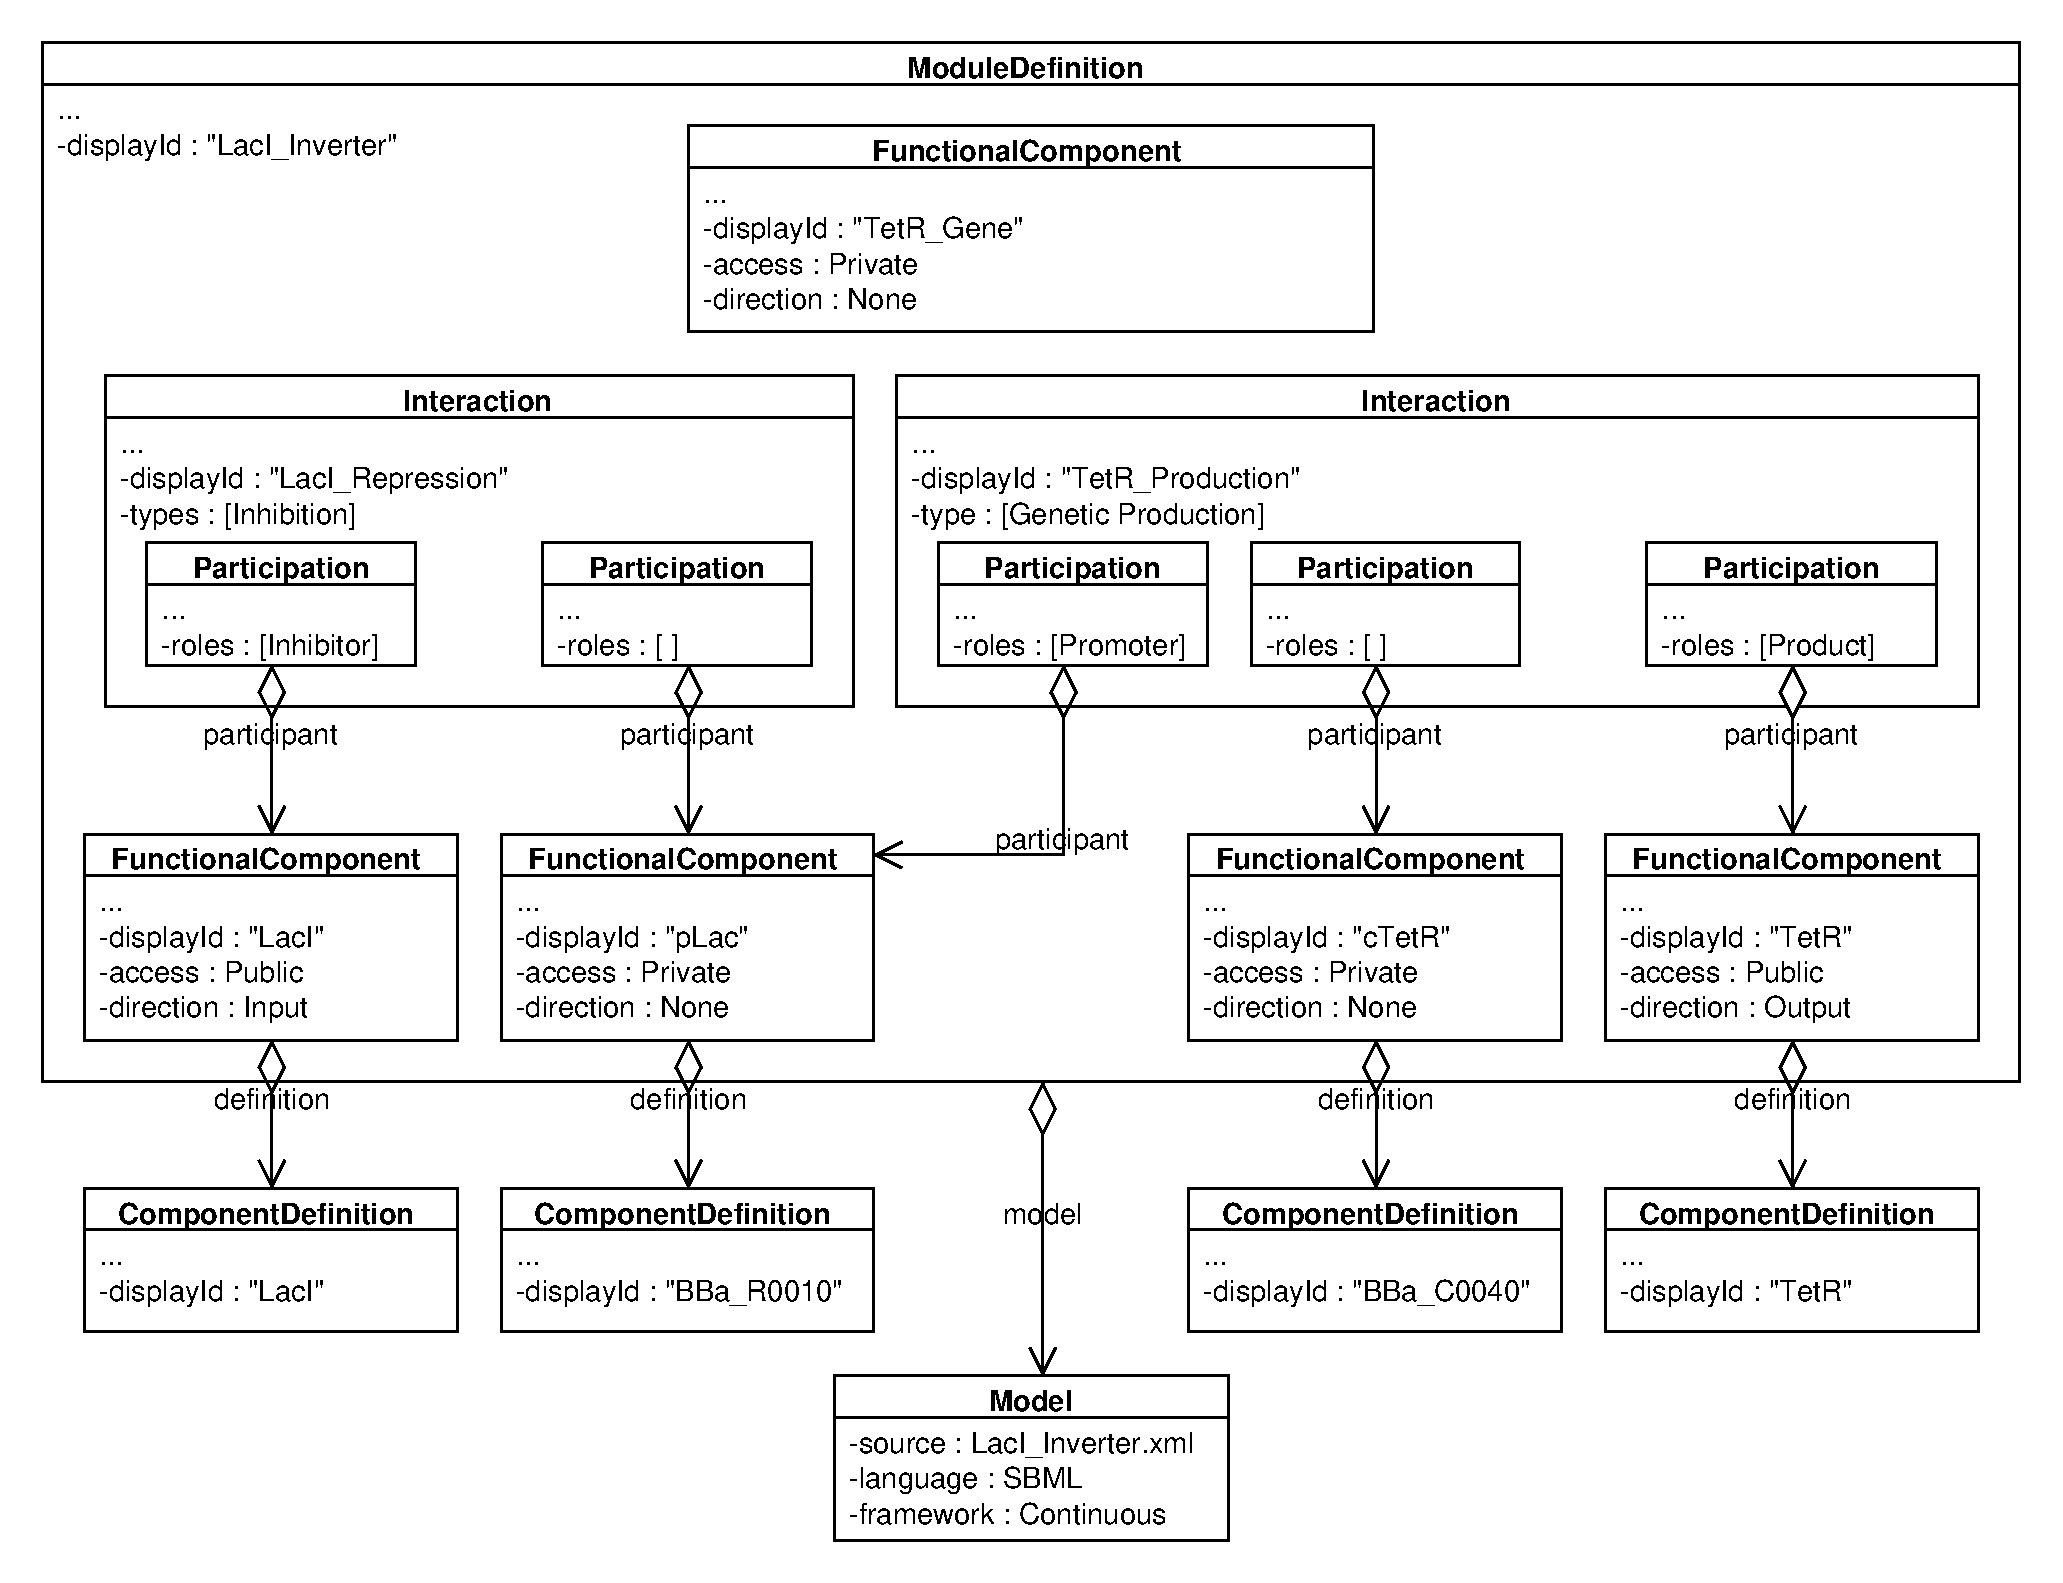
\includegraphics[width=\textwidth]{example_uml/toggle_3}
\caption[]{\sbol{ModuleDefinition} of the LacI inverter. This \sbol{ModuleDefinition} contains \sbol{FunctionalComponent} objects that instantiate the \sbol{ComponentDefinition} objects for the LacI/TetR transcription factors and TetR gene. The \sbol{FunctionalComponent} for the TetR gene as a whole does not participate in any \sbol{Interaction} and merely indicates the overall structure that is functionally described by the LacI inverter \sbol{ModuleDefinition}. The remaining \sbol{FunctionalComponent} objects participate in a repression \sbol{Interaction} and a genetic production \sbol{Interaction}, thereby indicating which parts of the overall structure carry out the function of the LacI inverter \sbol{ModuleDefinition}. In this case, the transcription and translation of TetR are represented as a single genetic production \sbol{Interaction} that abstracts away the presence of the intermediate TetR mRNA.  In addition, this \sbol{ModuleDefinition} is also associated with a continuous \sbol{Model} written in the SBML source file ``LacI\_Inverter.xml.''}
\label{uml:ex_mod_def}
\end{center}
\end{figure}

\begin{figure}[ht]
\begin{center}
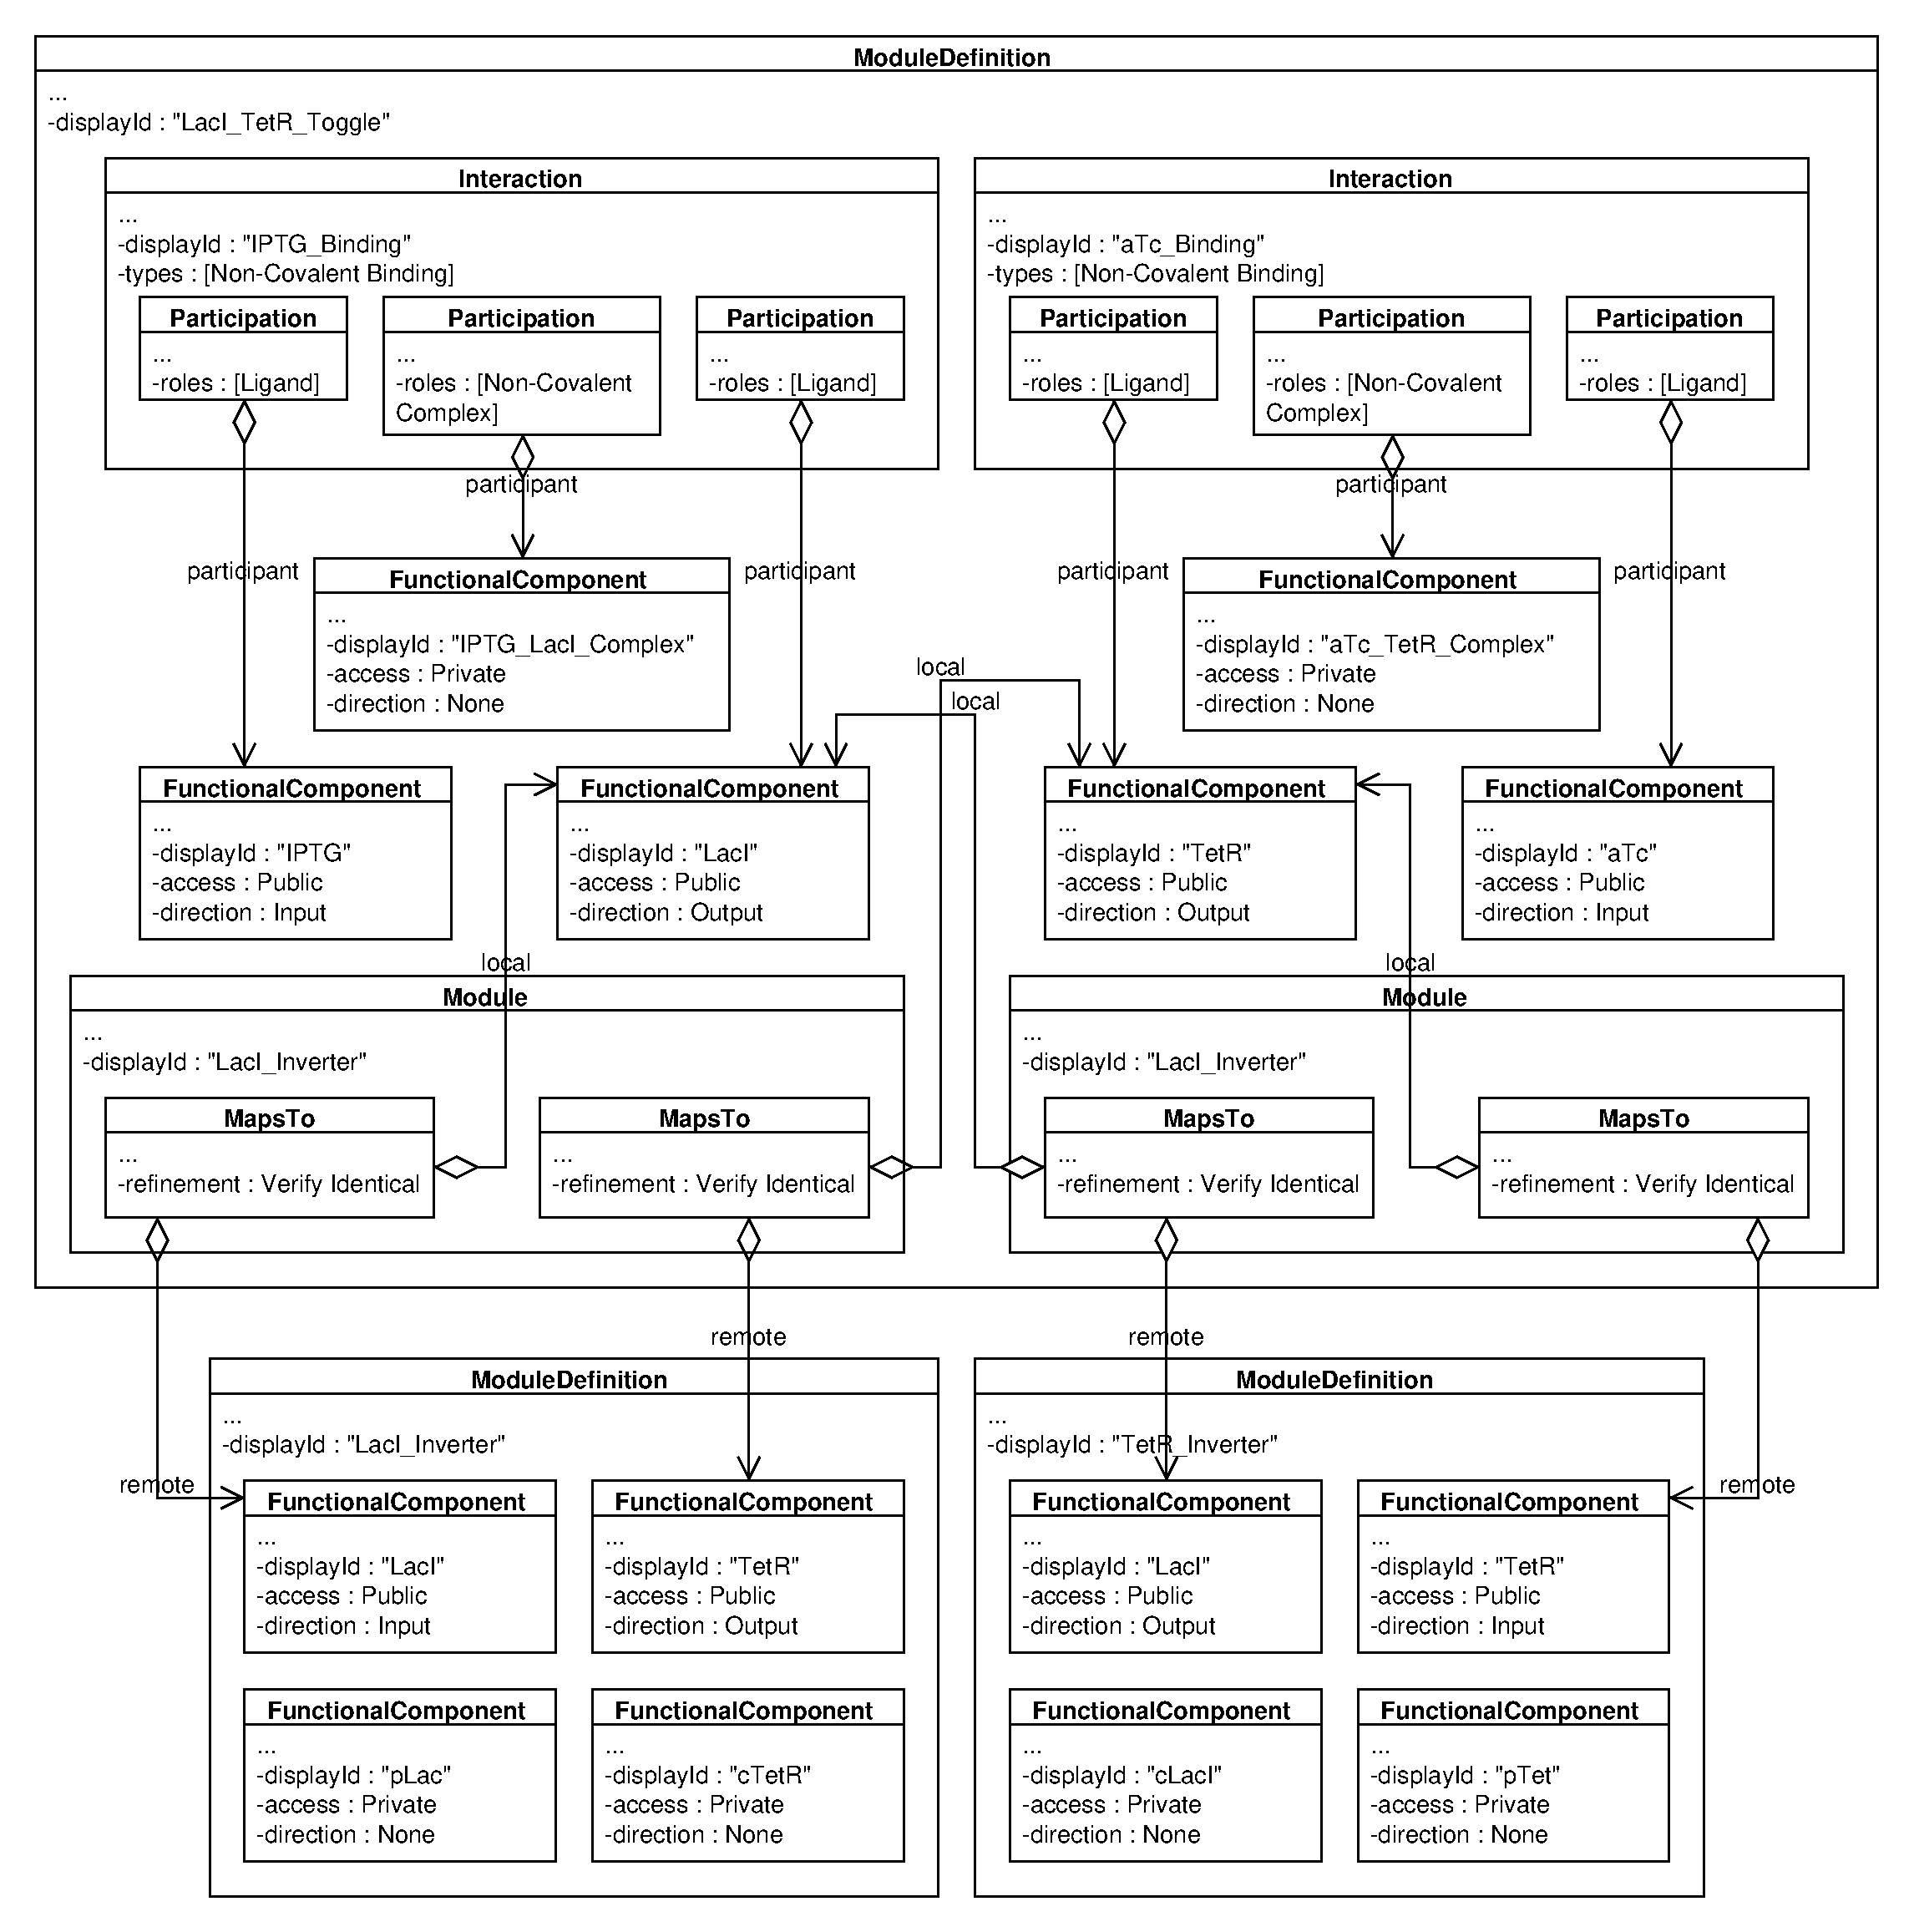
\includegraphics[width=\textwidth]{example_uml/toggle_4}
\caption[]{Composite \sbol{ModuleDefinition} of the LacI/TetR toggle switch. This \sbol{ModuleDefinition} contains the \sbol{Module} objects that instantiate \sbol{ModuleDefinition} object for sthe LacI and TetR inverter. It also contains \sbol{FunctionalComponent} objects that instantiate the \sbol{ComponentDefinition} objects for the LacI/TetR transcription factors and IPTG/aTc small molecules. These \sbol{FunctionalComponent} objects each participate in a non-covalent binding \sbol{Interaction}. To complete the composition of the toggle switch, \sbol{MapsTo} objects are used to indicate that the output of the LacI inverter \sbol{ModuleDefinition} is identical to the input of the TetR inverter \sbol{ModuleDefinition} and vice versa.
}
\label{uml:ex_mod_def_compo}
\end{center}
\end{figure}

% Each \sbol{ModuleDefinition} also contains the \sbol{FunctionalComponent}s that participate in \sbol{Interaction}s and are defined by the same \sbol{ComponentDefinition}s as the parallel \sbol{Component}s in the structural hierarchy of the toggle switch. Finally, \sbol{MapsTo} entities are used to refine which \sbol{FunctionalComponent}s of the functional hierarchy are identical or map them to \sbol{Component}s in the structural hierarchy.

\Rtodo{ComponentDefinition.types in the following figure are not consistent with the list of BioPax ontological terms described previously in the Data Model section. Should now be consistent. - Nic}

%  The first use case is to indicate with greater fidelity how a module describes the function of a composite component, namely by asserting that particular component instantiations within the module correspond to particular component instantiations within the component. 

% As an example of this use case, one might compose the structure and function of the LacI-repressible gene of the genetic toggle switch. In this example, the LacI-repressible gene and two of its subcomponents, the pLac promoter and cTetR CDS, are to be composed with the LacI inverter module. In order to compose these components with the LacI inverter module and indicate that it describes their behavior, they are instantiated inside the module. In addition, port maps are placed on the instantiation of the LacI-repressible gene to connect between its pLac plus cTetR subcomponent instantiations and the corresponding component instantiations in the module. Doing so makes it clear which subcomponent instantiations in the gene are being described by which component instantiations in the module. In this way, GDA tools for sequence editing and biochemical modeling can guarantee that their users are handling corresponding elements of a given genetic design, while GDA tools for genetic technology mapping can make explicit connections between the structural and functional elements of a design.

% -----------------------------------------------------------------------------
\section{SBOL RDF Serialization}
\label{sec:serialization}
% -----------------------------------------------------------------------------

\todo[inline]{try to target readers unfamiliar with RDF/XML.  -bder}

The SBOL serialization is designed to meet several competing requirements. Firstly, SBOL needs to support ad-hoc annotations and extensions. Secondly, SBOL needs to support processing by generic semantic web and database tools that have little or no knowledge of the SBOL data model. Thirdly, SBOL needs to support the generation of light-weight software clients so as to lower the barrier to entry for new API implementations within environments where community-maintained implementation(s) are not suitable.

The canonical serialization of SBOL is to a strict dialect of RDF/XML. This serialization provides the base from which to meet further requirements. Any RDF/XML-aware tooling can consume and analyze an SBOL file. Where possible, we have re-used predicates from widely-used terminologies (such as Dublin Core~\cite{dcmi2012}) to expose as much of the data as practical to standard RDF tooling.

Arbitrary RDF/XML provides a great deal of flexibility in how equivalent data can be serialized. This flexibility can result in different serializations when processing RDF/XML files using standard off-the-shelf XML tools, such as DOM-OO mappings. To address this problem, we define a canonical association between the nesting of data structures within the SBOL UML data model and the RDF/XML file. For all ownership associations (filled diamonds), the RDF/XML for the owned entity is embedded within the owner's RDF/XML. For all associations that are by reference (open diamonds), the RDF/XML for the referenced property is linked via a resource URI.

All first-class SBOL datatypes have an associated identity URI. In the RDF, this is the resource URI used by instances of that type. Properties and associations are asserted as nested RDF/XML assertions. Some datatypes are `top level,' which means that they always appear at the top level of the RDF/XML serialization. All other datatypes will always appear nested within their parent container.

Each instance of a first-class SBOL datatype may have annotations attached. These annotations are composed of a name and a value.  They are serialized to RDF as a triple with the subject being the identity of the instance they annotate, the predicate being the name of the annotation, and the object being the value of that annotation. Annotation values are always nested within the RDF/XML serialization of the instance that they annotate.

SBOL supports top-level, user-defined annotations. This is to allow non-standardized but necessary information to be carried around as part of a design. For example, a particular sub-community may have an internal standard for data sheets. Individual data sheets can be represented as a generic top-level annotation with internal structured annotations. This annotation will be serialized into the RDF/XML in the usual way, as a RDF/XML block at the top level of the file. Other objects may refer to this entity through their annotations by reference, and this generic top-level entity may refer to other entities via references.

By adopting this paradigm of RDF/XML serialization, SBOL is able to adapt to future changes in the standard without requiring large-scale alterations to the RDF files. Since exactly the same scheme is used to serialize annotations as is used to serialize specification-defined properties and associations, it is possible to update the SBOL standard to recognize a different range of properties and associations. Those properties not recognized by the specification will always be available through the API as annotations. Similarly, by allowing arbitrary top-level entities in an SBOL file, we enable future specifications or extensions to ratify the structure of . These entities would then become part of the explicit data model, but the identical RDF serialization would be used. Applications lacking support for a given extension can safely round-trip the top-level data that is not understood, treating it as a top-level structured annotation, without data loss or corruption. The very regimented control of nesting versus referencing allows the XML structure to be very predictable, enabling XML/DOM-based tooling to work with SBOL RDF/XML files safely.


\section{SBOL Compliance}

There are different types of software compliance with respect to the SBOL specification.  First, a software tool can either support all classes of the SBOL 2.x data model or only its structural subset.  The structural subset includes the following classes:
\begin{itemize}
\item \sbol{Sequence}
\item \sbol{ComponentDefinition}
\begin{itemize}
\item \sbol{Component}
\item \sbol{SequenceAnnotation}
\item \sbol{SequenceConstraint}
\end{itemize}
\item \sbol{Collection}
\item \sbol{Annotation}
\item \sbol{GenericTopLevel}
\end{itemize}
Second, an SBOL-compliant software tool can support import of SBOL, export of SBOL, or both.  
If it supports both import and export, it can do so in either a lossy or lossless fashion.

In order to test import compliance, developers are encouraged to use the SBOL test files found here:\\ {\url{https://github.com/SynBioDex/SBOLTestSuite}}\\
Examples of every meaningful subset of objects are provided, including both structural-only SBOL (that is, annotated DNA sequence data) and complete tests.  

In order to test export compliance, developers are encouraged to validate SBOL files generated by their software with the SBOL Validator found here:\\
\url{http://www.async.ece.utah.edu/sbol-validator/}\\
This validator can also be used to check lossless import/export support, since it can compare the data content of files imported and exported by a software tool.

Finally, developers of SBOL-compliant tools are encouraged to notify the SBOL editors\\(sbol-editors@googlegroups.com) when they have determined that their tool is SBOL compliant, so their tool can be publicly categorized as such on the SBOL website.




\section{Mapping Between SBOL 1, SBOL 2, and SBOL3}
\label{sec:mapping}

In broad strokes, the SBOL 1 standard focused on conveying physical, structural information, whereas SBOL 2 expanded the scope to include functional aspects as well.  
The physical information about a designed genetic construct includes the order of its constituents and their descriptions. 
Specifying the exact locations of these constituents and their sequences allows genetic constructs to be defined unambiguously and reused in other designs. 
SBOL 2 extended SBOL 1 in several ways: it extends physical descriptions to include entities beyond DNA sequences, and it added support for functional descriptions of designs.  
SBOL 3 refined the data model to simplify the representation of common use cases.

\subsection{Mapping between SBOL 1 and SBOL 2}

\ref{SBOL1TO2} depicts the mapping of SBOL 1.1 classes to SBOL 2.x classes, indicating corresponding classes/properties by color.
The SBOL 2.x \sbol{Model} and \sbol{CompenentDefinition} classes have no SBOL 1.1 equivalent, and thus are not shown.
In particular:
\begin{itemize}
\item SBOL 1.1 \external{Collection} objects containing \external{DnaComponent} objects map to SBOL 2.x \sbol{Collection} objects that contain \sbol{CompenentDefinition} objects with DNA \sbolmult{types:CD}{types} properties.
\item SBOL 1.1 \external{DnaComponent} objects maps to SBOL 2.x \sbol{CompenentDefinition} objects with DNA \sbolmult{types:CD}{types} properties.
\item SBOL 1.1 \external{DnaSequence} objects maps to an SBOL 2.x \sbol{Sequence} objects with \external{IUPAC DNA} \sbol{encoding} properties.
\item SBOL 1.1 \external{SequenceAnnotation} objects with \external{bioStart} and \external{bioEnd} properties map to SBOL 2.x\\
\sbol{SequenceAnnotation} objects that contain \sbol{Range} objects.
\item SBOL 1.1 \external{SequenceAnnotation} objects that lack \external{bioStart} and \external{bioEnd} properties map to an SBOL 2.x \sbol{SequenceFeature} objects that contain \sbol{GenericLocation} objects.
\item Each SBOL 1.1 \external{SequenceAnnotation} also maps to an SBOL 2.x \sbol{Component}, which represents the instantiation or usage of the appropriate \sbol{CompenentDefinition}.
\item Each SBOL 1.1 \external{precedes} property maps to an SBOL 2.x \sbol{SequenceConstraint} that specifies a precedes \sbol{restriction} property.
\end{itemize}

\begin{figure*}[h]
\begin{center}
  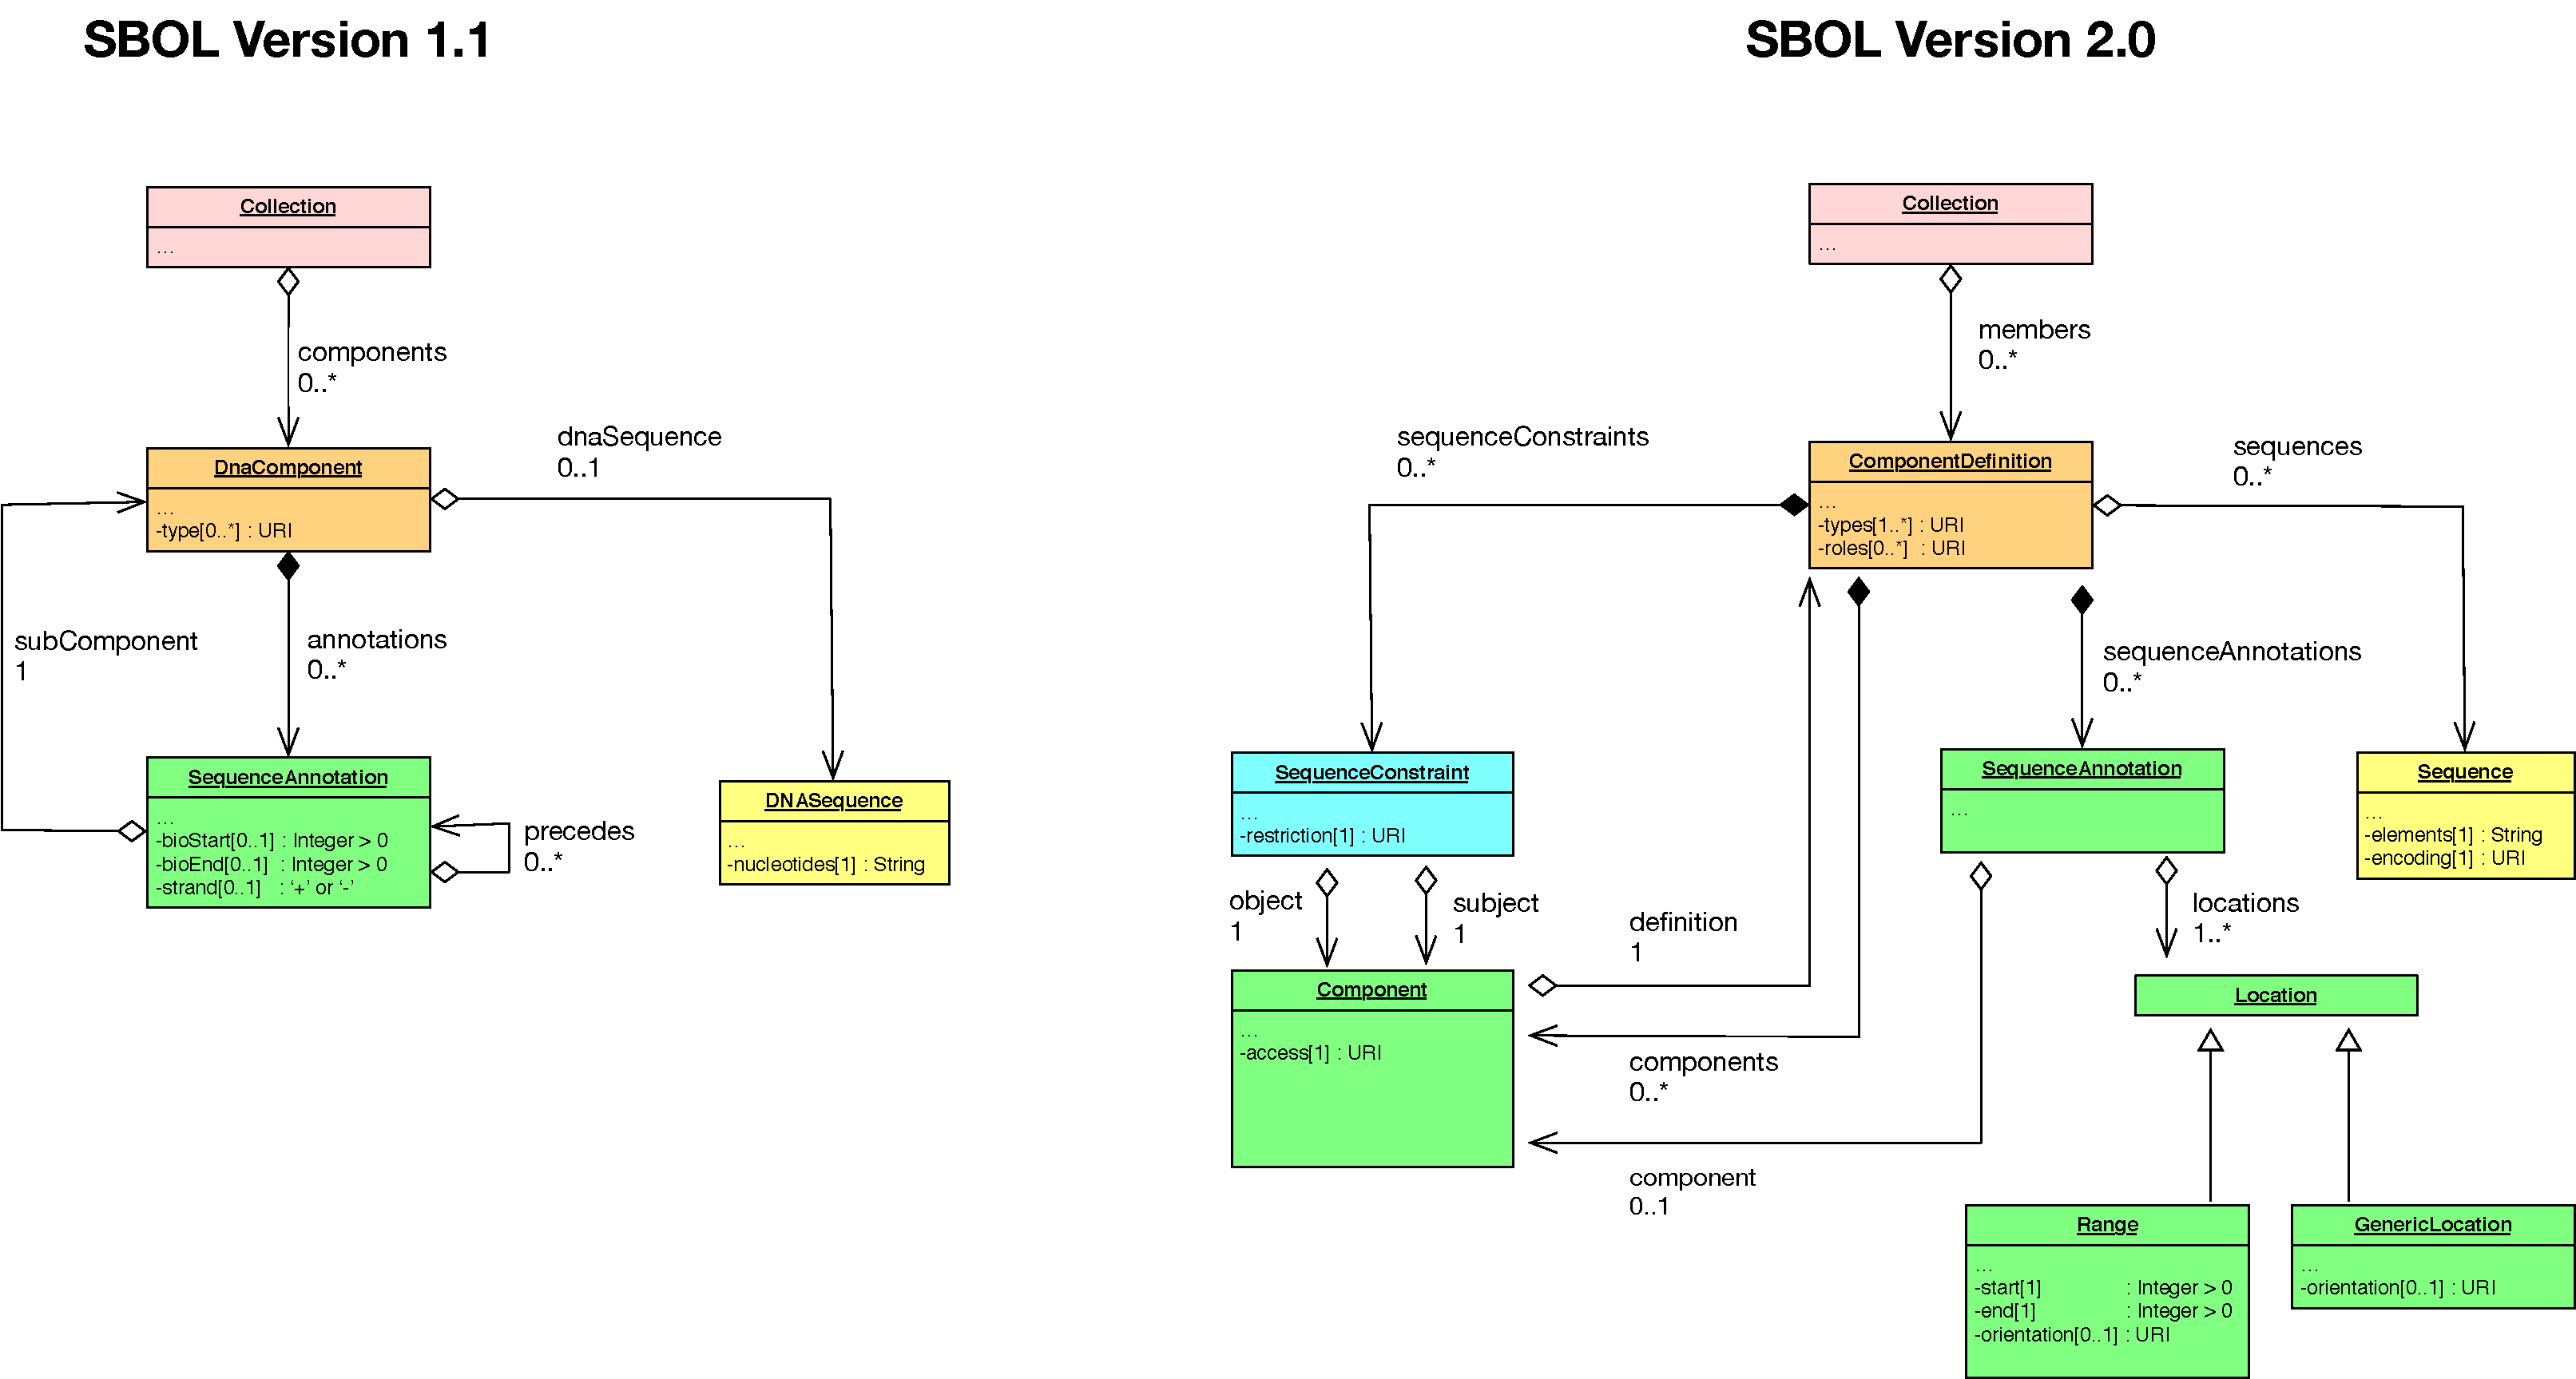
\includegraphics[width=\textwidth]{images/sbol_v1_to_v2}
\end{center}
\caption{\label{SBOL1TO2}The mapping from the SBOL 1.1 data model to the SBOL 2.x  data model, indicating corresponding classes/properties by color.}
\end{figure*}

\subsection{Mapping between SBOL 2 and SBOL 3}

\ref{SBOL1TO2} depicts the mapping of SBOL 2.3 classes to SBOL 3.x classes, indicating corresponding classes/properties by color.

\begin{itemize}
    \item SBOL 2.x \external{ComponentDefinition} objects map to SBOL 3.x \sbol{Component} objects.  The \sbol{type} property is mapped according to  \ref{tbl:component_type_mapping}.
    \item SBOL 2.x \external{ModuleDefinition} objects map to SBOL 3.x \sbol{Component} objects with a \sbol{type} of \texttt{SBO:0000241} (functional entity)
    \item Every \external{FunctionalComponent} in an SBOL 2.x \external{ModuleDefinition} with a "direction" property that is not "none" is listed in the \sbol{Interface} of its SBOL 3.x \sbol{Component}. The mapping from direction to interface properties is: "in"-->"inputs", "out"-->"outputs", "inout" --> "nondirectional". Finally, every Component with "access"="public" and "direction"="none" is listed as "nondirectional" in the Interface.
    \item Every \external{Component} in an SBOL 2.x \external{ComponentDefinition} with "access"="public" is listed as "nondirectional" in the \sbol{Interface} of its SBOL 3.x \sbol{Component}.
    \item SBOL 2.x \external{Component}, \external{Module}, and \external{FunctionalComponent} objects map to SBOL 3.x \sbol{SubComponent} objects
    \item SBOL 2.x \external{SequenceConstraint} objects map to SBOL 3.x \sbol{Constraint} objects
    \item SBOL 2.x \external{MapsTo} objects with a value other than \external{merge} are converted to an SBOL 3.x \sbol{Constraint}. \todo{Jake: please can you provide more detail?}
    \item SBOL 2.x \external{SequenceAnnotation} objects map to SBOL 3.x \sbol{SequenceFeature} objects if they do not have a \external{component}. If they do have a \external{component}, their locations are added to the corresponding SBOL3 \sbol{SubComponent}.
    \item \external{Location} objects are assigned an \sbol{order} integer.  In the case of multiple locations, the order may be inferred, e.g. from the \external{start} and \external{end} properties of ranges.  However, such behaviour is tooling-specific.
\end{itemize}

\begin{table}[ht]
  \begin{edtable}{tabular}{ll}
    \toprule
    \textbf{SBOL 2.x Type} & \textbf{SBOL 3.x Type} \\
    \midrule
      \url{http://www.biopax.org/release/biopax-level3.owl\#Dna} & \url{https://identifiers.org/SBO:0000251 (DNA)}\\
      \url{http://www.biopax.org/release/biopax-level3.owl\#DnaRegion} & \url{https://identifiers.org/SBO:0000251} (DNA)\\
      \url{http://www.biopax.org/release/biopax-level3.owl\#Rna} & \url{https://identifiers.org/SBO:0000250} (RNA)\\
      \url{http://www.biopax.org/release/biopax-level3.owl\#RnaRegion} & \url{https://identifiers.org/SBO:0000250} (RNA)\\
      \url{http://www.biopax.org/release/biopax-level3.owl\#Protein} & \url{https://identifiers.org/SBO:0000252} (Protein)\\
      \url{http://www.biopax.org/release/biopax-level3.owl\#SmallMolecule} & \url{https://identifiers.org/SBO:0000247} (Simple Chemical)\\
      \url{http://www.biopax.org/release/biopax-level3.owl\#Complex} & \url{https://identifiers.org/SBO:0000253} (Non-covalent Complex)\\
    \bottomrule
  \end{edtable}
  \caption{Mapping of SBOL2 ComponentDefinition types to SBOL3 Component types}
 \label{tbl:component_type_mapping}
\end{table}:

\begin{figure*}[h]
	\begin{subfigure}{.5\textwidth}
		\centering
		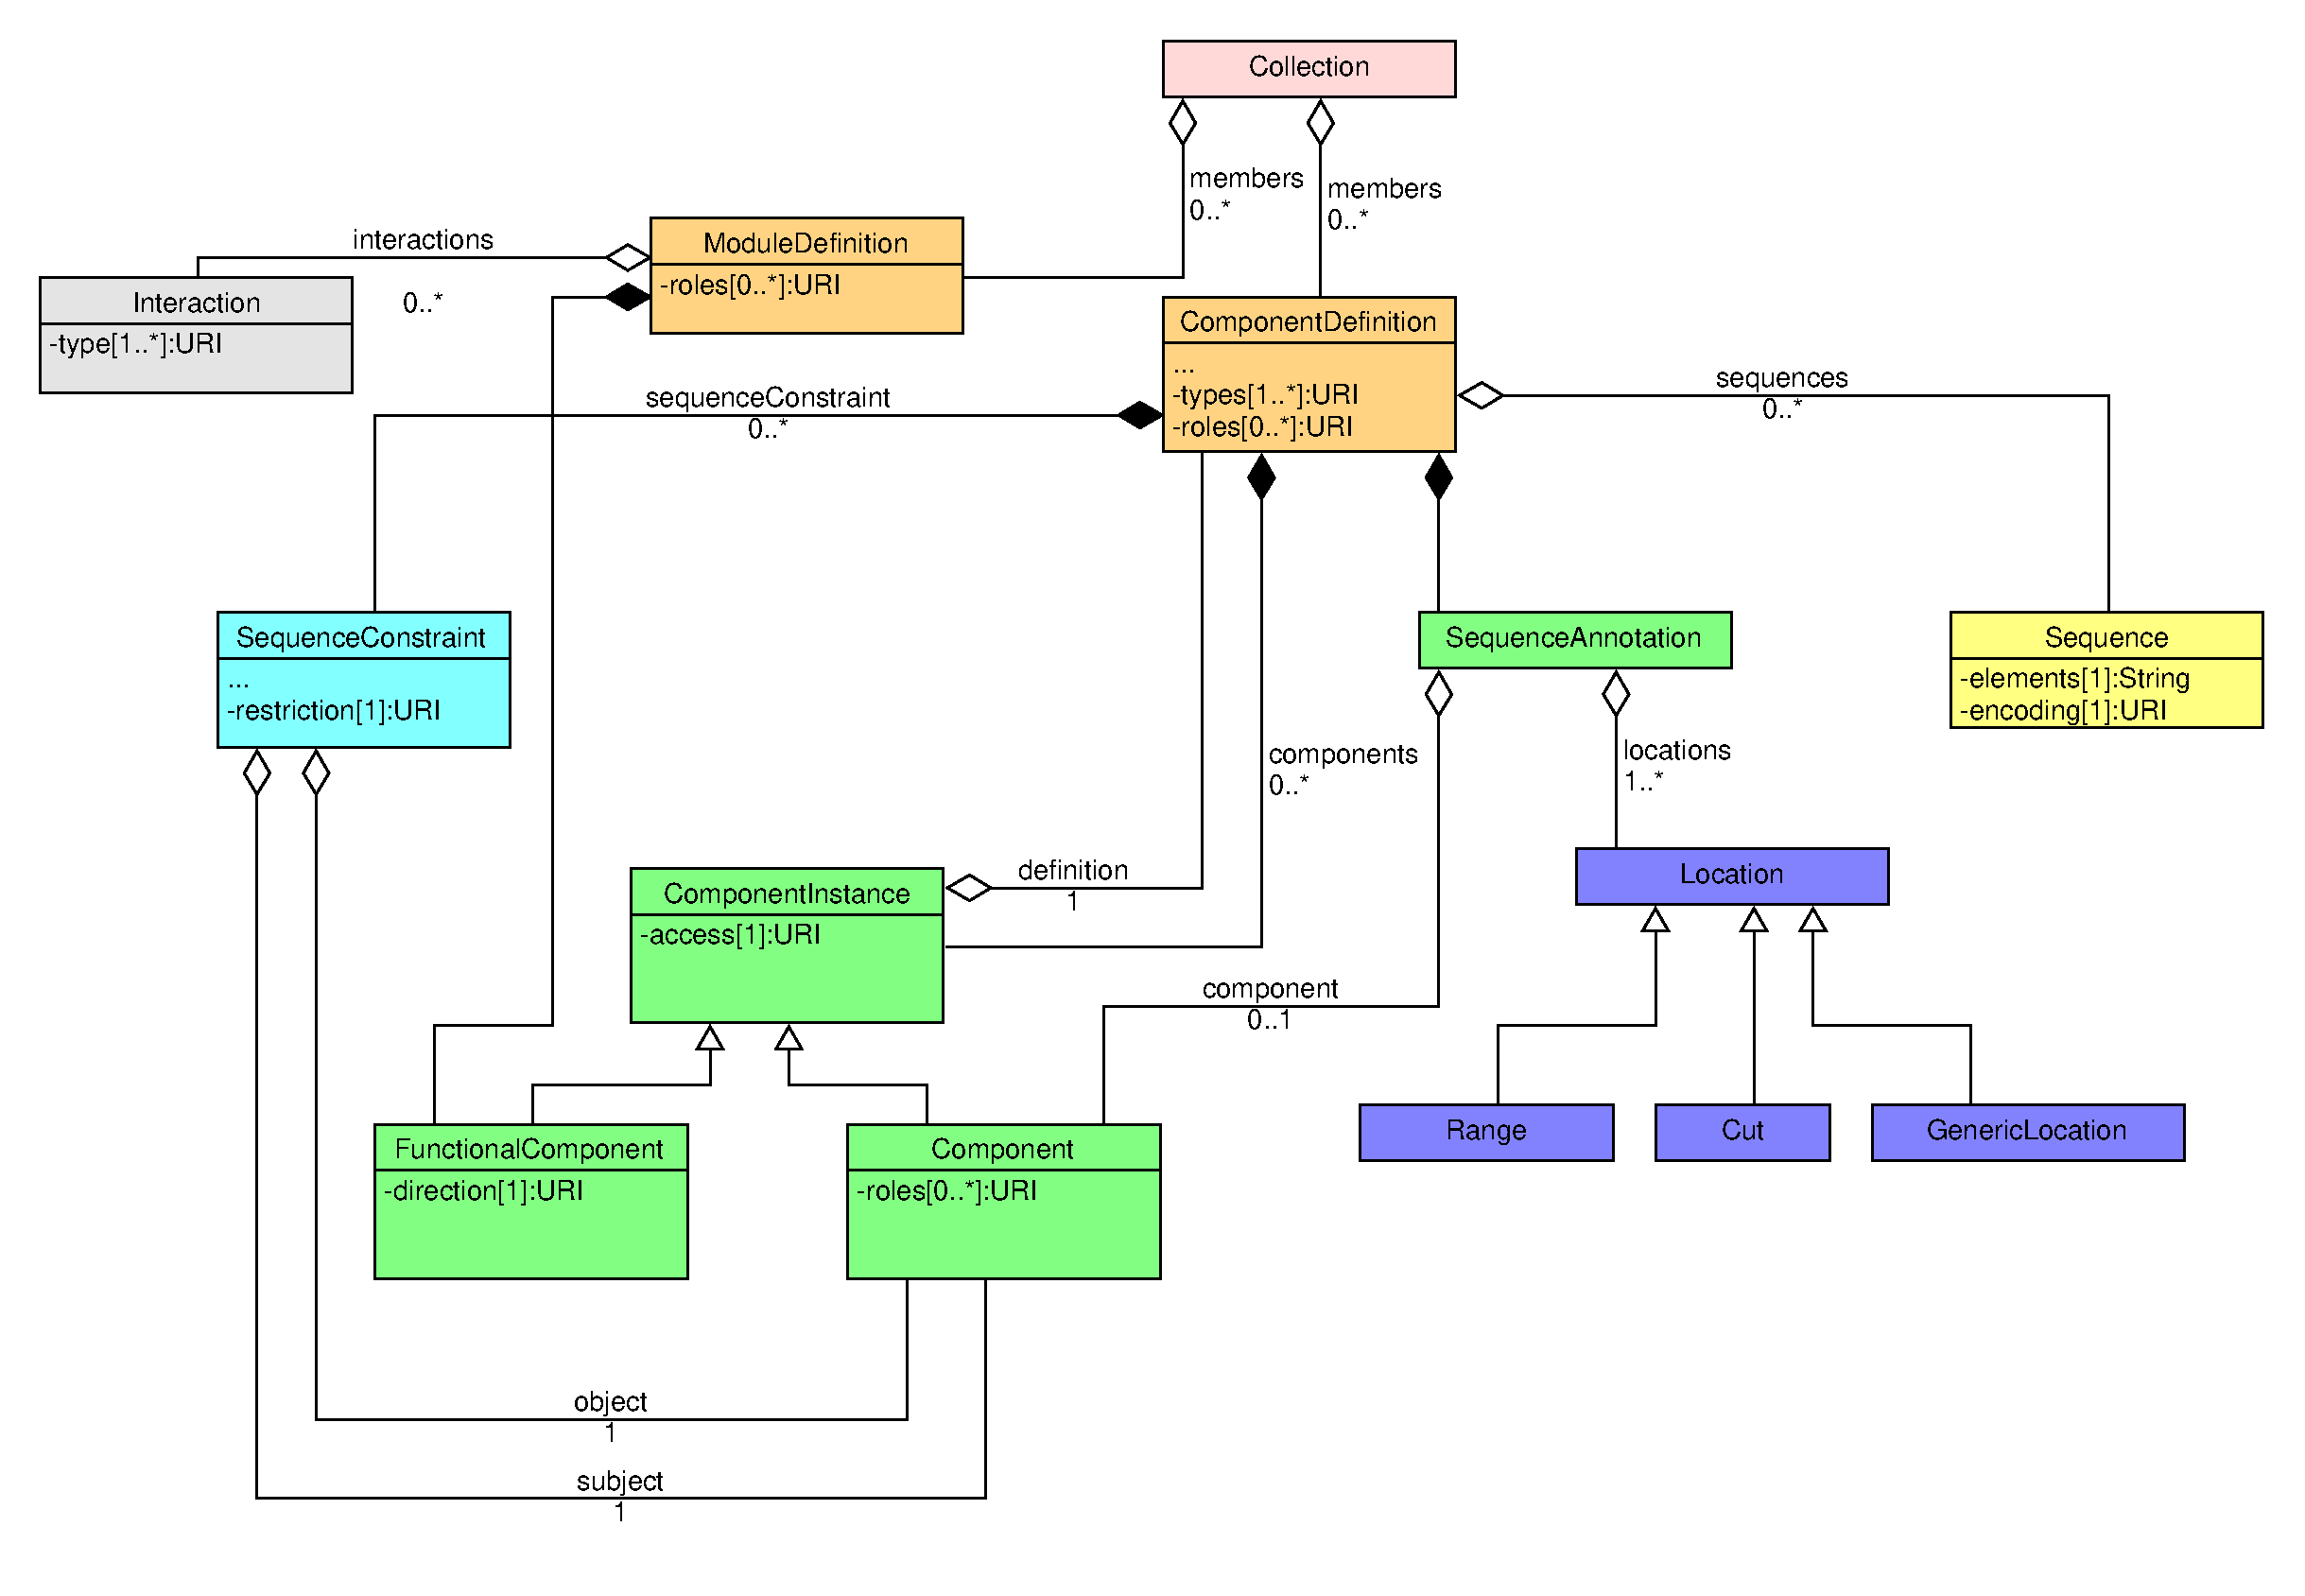
\includegraphics[width=\linewidth]{images/sbol_v2_to_v3_left_subfigure}  
		\caption{SBOL 2.3}
		\label{fig:sub-first}
	\end{subfigure}\begin{subfigure}{.5\textwidth}
		\centering
		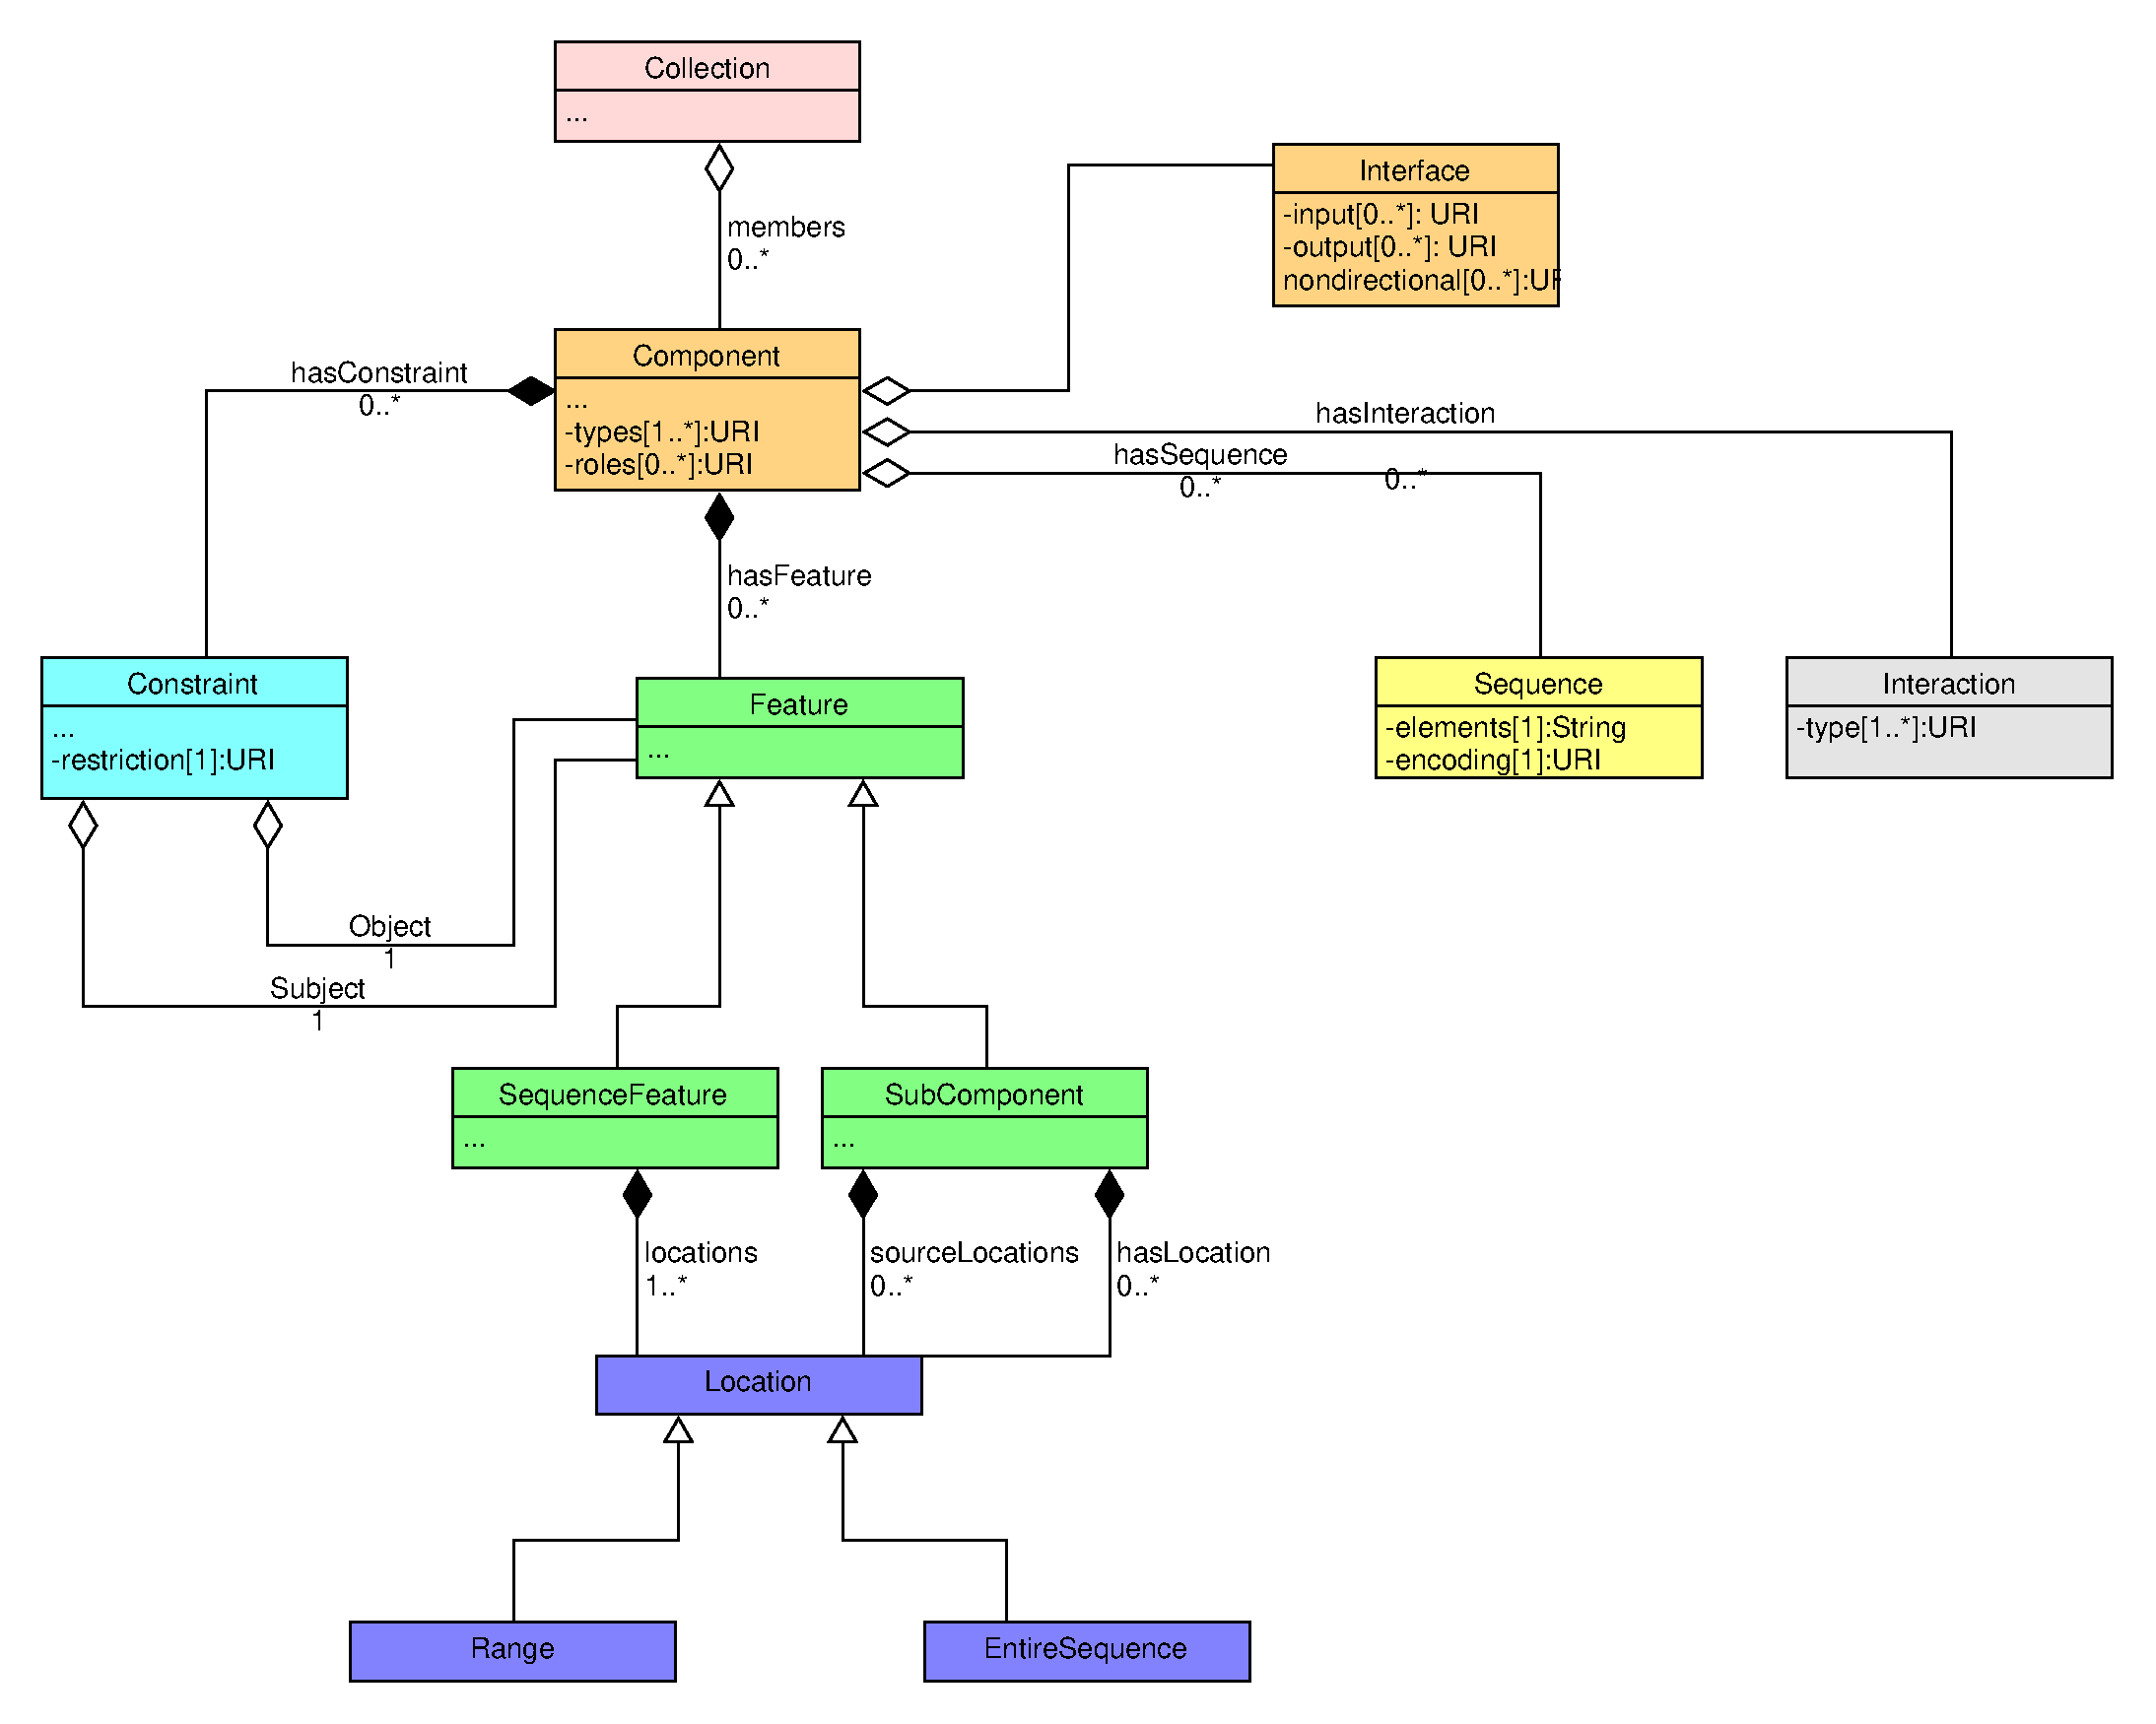
\includegraphics[width=\linewidth]{images/sbol_v2_to_v3_right_subfigure}  
		\caption{SBOL 3.x}
		\label{fig:sub-second}
	\end{subfigure}
	\caption{\label{SBOL2TO3}The mapping from the SBOL 2.3 data model to the SBOL 3.x  data model, indicating corresponding classes/properties by color.}
\end{figure*}




\newpage
\bibliography{sbol}

\appendix

% -----------------------------------------------------------------------------
\section{Complementary Standards}
\label{sec:complementaryStandards}
% -----------------------------------------------------------------------------
\subsection{Adding Provenance with PROV-O}
\label{sec:provenance}
\label{sec:prov:Entity}

The PROV-O ontology (\url{https://www.w3.org/ns/prov#}) defines a complementary data model that is leveraged by SBOL to describe provenance. Provenance is central to a range of workflow management, quality control, and attribution tasks within the Synthetic Biology design process. Tracking attribution and derivation of one resource from another is paramount for managing intellectual property purposes. Source designs are often modified in systematic ways to generate derived designs, for example, by applying codon optimization or systematically removing all of a class of restriction enzyme sites.  Documenting the transformation used, and any associated parameters, makes this explicit and potentially allows the process to be reproduced systematically. If a design has been used within other designs, and is later found to be defective, it is paramount that all uses of it, including uses of edited versions of the design, can be identified, and ideally replaced with a non-defective alternative. When importing data from external sources, it is important not only to attribute the original source (for example, GenBank), but also the tool used to perform the import, as this may have made arbitrary choices as to how to represent the source knowledge as SBOL. All these activities have in common that it is necessary to track what resource, and what transformation process was applied by whom to derive an SBOL design.

This section describes a minimal subset of PROV-O terms and classes that may be used by SBOL tools to support representation of provenance\footnote{We thank Dr Paolo Missier from the School of Computing Science, Newcastle University for discussions regarding the use of PROV-O.}. Although the full-set of PROV-O terms can be used in SBOL documents, a subset of PROV-O is adopted as a best practice. It is advised that SBOL tools should at least understand this subset, defined in \ref{uml:provenance}. Providers of provenance information are free to make use of more of PROV-O than is described here. It is acceptable for tools that understand more than this subset to use as much as they are able. Tools that only understand this subset must treat any additional data as annotations. Tools that are not aware of SBOL provenance at all MUST maintain and provide access to this information as annotations. This specification does not state what the newly added properties must point to. As long as they are resources that are consistent with the PROV-O property domains, they are legal. For example, a \sbol{Component} may be derived from another \sbol{Component}, but it would probably not make sense for it to be derived from a \sbol{Collection}.

The most basic and general type of provenance relationship can be represented using the \prov{wasDerivedFrom} property. This relationship describes derivation of an SBOL entity from another. 
Any \sbol{Identified} object may be annotated with this property. More specific provenance relationships can also be defined using PROV-O, such as \prov{wasGeneratedBy}. Generation of a new object is defined by the W3C PROV-O specification as follows:
\begin{quote}
	...the completion of production of a new entity by an activity. This entity did not exist before generation and becomes available for usage after this generation.
\end{quote}
These relationships are leveraged in SBOL tooling for describing multi-stage synthetic biology workflows.

Synthetic biology workflows may involve multiple stages, multiple users, multiple organizations, and interdisciplinary collaborations. These workflows can be described using four core PROV-O classes: \prov{Entity}, \\ \prov{Activity}, \prov{Agent}, and \prov{Plan}. Any SBOL \sbol{Identified} object can implicitly act as an instance of PROV-O's \prov{Entity} class. Workflow histories (retrospective provenance) and workflow specifications (prospective provenance) can be described in SBOL using \prov{Activity} objects to link \sbol{Identified} objects into workflows. An \prov{Agent} (for example a software or a person) runs an \prov{Activity} according to a \prov{Plan} to generate new entities. Resources representing \prov{Agent}, \prov{Activity} and \prov{Plan} classes should be handled as \sbol{TopLevel}, whilst \prov{Usage} and \prov{Association} resources should be treated as child \sbol{Identified} objects within their parent \prov{Activity} objects.  

A design-build-test-learn SBOL ontology has been adopted for use with PROV-O classes (see \ref{tbl:activity_types}). The terms \textit{design}, \textit{build}, \textit{test}, and \textit{learn} provide a high level workflow abstraction that allows tool-builders to quickly search for and isolate provenance histories relevant to their domain, while keeping track of the flow of data between different users working in different domains of synthetic biology. These terms SHOULD BE used on the \sbolmult{type:Activity}{type} property of the \prov{Activity} class. (Note that this property is a special property added by the SBOL specification, and is not part of the original PROV-O specification.) Additionally, these terms SHOULD BE used in the \provmult{hadRole:U}{hadRole} properties on \prov{Usage} to qualify how the referenced \prov{entity} is used by the parent \prov{Activity}. 

\begin{table}[ht]
	\begin{edtable}{tabular}{llp{3.5in}}
		\toprule
		\textbf{Activity Type} & \textbf{URI}  & \textbf{Description}\\
		\midrule
		Design  & \url{http://sbols.org/v3\#design}  & Design describes the process by which a conceptual representation of an engineer's imagined and intended design for a biological system is created or derived.\\
		Build  & \url{http://sbols.org/v3\#build}  & Build describes the process by which a biological construct, sample, or clone is implemented in the laboratory.\\
		Test  & \url{http://sbols.org/v3\#test} & Test describes the process of performing experimental measurements to characterize a synthetic biological construct.\\
		Learn  & \url{http://sbols.org/v3\#learn} & Learn describes the process of analyzing experimental measurements to produce a new entity that represents biological knowledge.\\
		\bottomrule
	\end{edtable}
	\caption{Synthetic biology workflow ontology}
	\label{tbl:activity_types}
\end{table}

Logical constraints are placed on the order in which different types of \prov{Activity}s are chained into design-build-test-learn workflows. These rules additionally place constraints on the types of objects that may be used as inputs for a particular type of \prov{Activity}. For example, a \textit{design} \prov{Usage} may be used as an input for either a \textit{design} or \textit{build} \prov{Activity} but SHOULD NOT be used as an input for a \textit{test} \prov{Activity}. An example of how these terms are used is provided in \ref{images:design-build-test-learn}. 
The ordering of stages and constraints on referred object type are given in \ref{tbl:dbtl_stages}.

\begin{table}[ht]
\begin{tabular}{lll}
\toprule
\textbf{Stage} & \textbf{Preceding Stage} & \textbf{Referred Object Type} \\
\midrule
\url{http://sbols.org/v3\#design}	& \url{http://sbols.org/v3\#learn}		& \sbol{TopLevel} other than \sbol{Implementation} \\
\url{http://sbols.org/v3\#build}	& \url{http://sbols.org/v3\#design}	& \sbol{Implementation} \\
\url{http://sbols.org/v3\#test}	& \url{http://sbols.org/v3\#build}		& \sbol{ExperimentalData} \\
\url{http://sbols.org/v3\#learn}	& \url{http://sbols.org/v3\#test}		& \sbol{Identified} other than \sbol{Implementation} \\
\bottomrule
\end{tabular}
\caption{Ordering of design-build-test-learn stages, and the types of objects RECOMMENDED to be associated with them.}
\label{tbl:dbtl_stages}
\end{table}


In addition to the design-build-test-learn terms, users may also wish to include more specific terms to specify how SBOL objects are used in-house in their own recipes, protocols, or computational analyses. In fact, it is expected that the SBOL workflow ontology will be expanded over time, as users experiment with and develop their own custom ontologies. For now, however, it is RECOMMENDED that SBOL tools also include the high-level terms in \ref{tbl:activity_types} to support data exchange across interdisciplinary boundaries.

\begin{figure}[ht]
\begin{center}
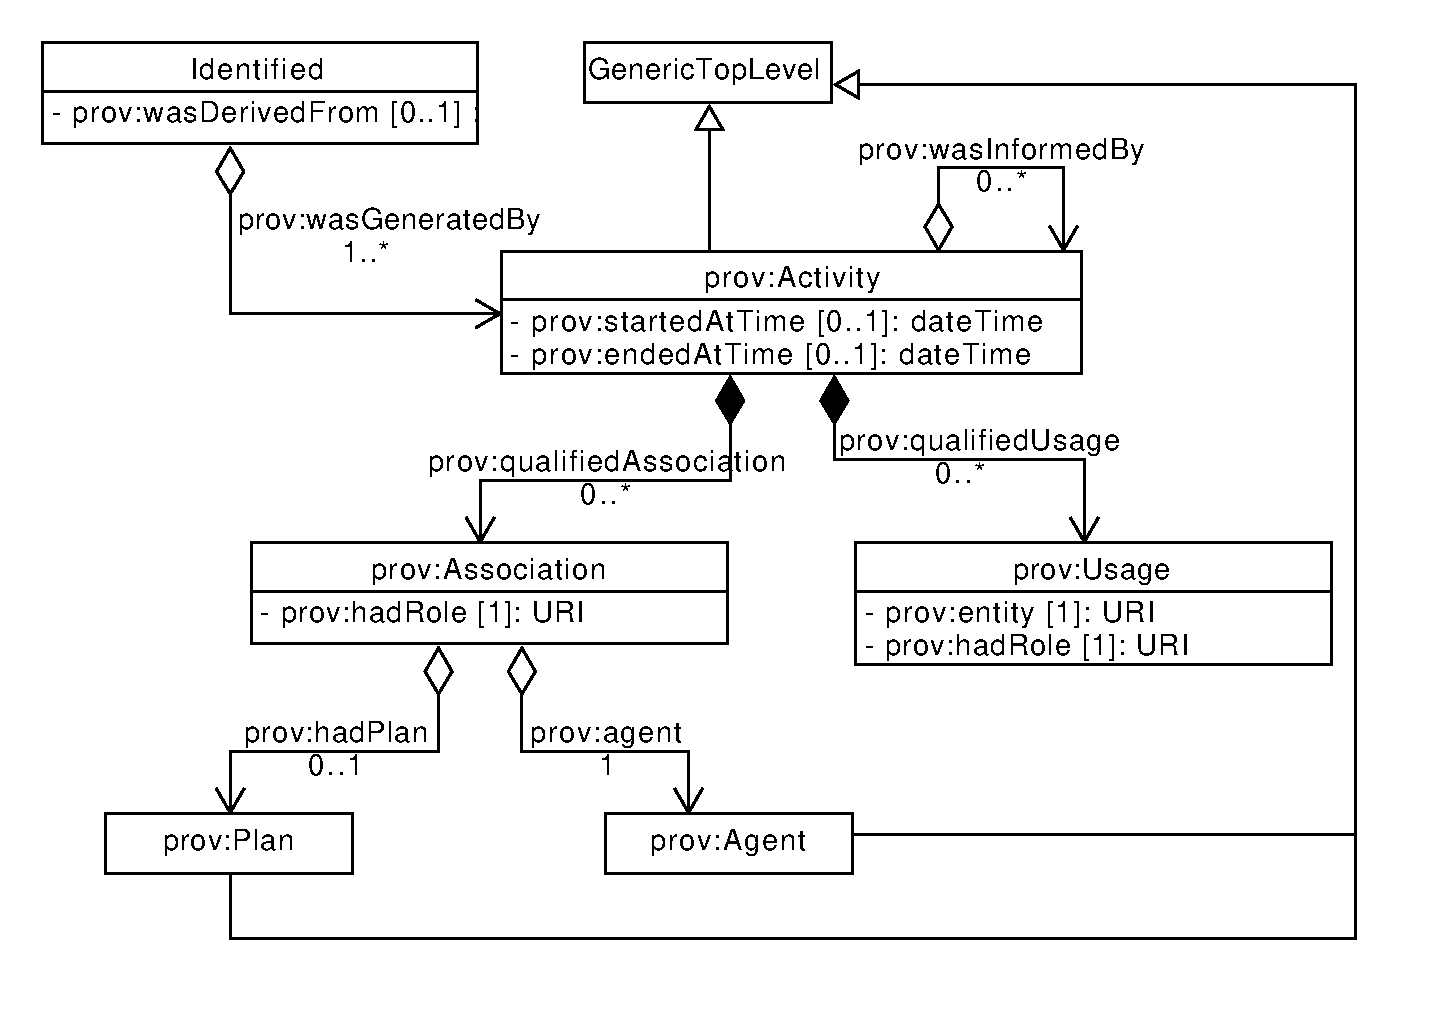
\includegraphics[scale=0.6]{uml/provenance}
\caption[]{Relationships between SBOL and PROV-O classes. The PROV-O classes \external{prov:Activity}, \external{prov:Plan}, and \external{prov:Agent} all derive from \sbol{TopLevel} in the context of the SBOL data model.
\label{uml:provenance}}
\end{center}
\end{figure}

\subsubsection{prov:Activity}
\label{sec:prov:Activity}

A generated \prov{Entity} is linked through a \prov{wasGeneratedBy} relationship to an \prov{Activity}, which is used to describe how different \prov{Agent}s and other entities were used. An \prov{Activity} is linked through a \prov{qualifiedAssociation} to \prov{Association}s, to describe the role of agents, and is linked through \\ \prov{qualifiedUsage} to \prov{Usage}s to describe the role of other entities used as part of the activity. Moreover, each \prov{Activity} includes optional \prov{startedAtTime} and \prov{endedAtTime} properties. When using \prov{Activity} to capture how an entity was derived, it is expected that any additional information needed will be attached as annotations. This may include software settings or textual notes. Activities can also be linked together using the \prov{wasInformedBy} relationship to provide dependency without explicitly specifying start and end times.

\subparagraph{The \sbolheading{type} property}\label{sec:type:Activity}

An \prov{Activity} MAY have one or more \sbolmult{type:Activity}{type} properties, each of type \sbol{URI} that explicitly specifies the type of the provenance \prov{Activity} in more detail.  If specified, it is RECOMMENDED that at least one \sbolmult{type:Activity}{type} property refers to a \sbol{URI} from \ref{tbl:activity_types}.

\subparagraph{The \sbolheading{prov:startedAtTime} property}\label{sec:prov:startedAtTime}

The \prov{startedAtTime} property is OPTIONAL and contains a DateTime (see~\ref{sec:DateTime}) value, indicating when the activity started.  If this property is present, then the \prov{endedAtTime} property is REQUIRED.

\subparagraph{The \sbolheading{prov:endedAtTime} property}\label{sec:prov:endedAtTime}

The \prov{endedAtTime} property is OPTIONAL and contains a DateTime (see~\ref{sec:DateTime}) value, indicating when the activity ended.

\subparagraph{The \sbolheading{prov:qualifiedAssociation} property}\label{sec:prov:qualifiedAssociation}

An \prov{Activity} MAY have one or more \prov{qualifiedAssociation} properties, each of type \sbol{URI} that refers to an \prov{Association} object.

\subparagraph{The \sbolheading{prov:qualifiedUsage} property}\label{sec:prov:qualifiedUsage}

An \prov{Activity} MAY have one or more \prov{qualifiedUsage} properties, each of type \sbol{URI} that refers to an \prov{Usage} object.

\subparagraph{The \sbolheading{prov:wasInformedBy} property}\label{sec:prov:wasInformedBy}

An \prov{Activity} MAY have one or more \prov{wasInformedBy} properties, each of type \sbol{URI} that refers to another \prov{Activity} object.

\subsubsection{prov:Usage}
\label{sec:prov:Usage}

How different entities are used in an \prov{Activity} is specified with the \prov{Usage} class, which is linked from an \prov{Activity} through the \prov{Usage} relationship. A \prov{Usage} is then linked to an \prov{Entity} through the \prov{entity} property \sbol{URI} and the \provmult{hadRole:U}{hadRole} property species how the \prov{Entity} is used.  When the \prov{wasDerivedFrom} property is used together with the full provenance described here, the entity pointed at by the \prov{wasDerivedFrom} property MUST be included in a \prov{Usage}.

\subparagraph{The \sbolheading{prov:entity} property}\label{sec:prov:entity}

The \prov{entity} property is REQUIRED and MUST contain a \sbol{URI} which MAY refer to an \sbol{Identified} object.

\subparagraph{The \sbolheading{prov:hadRole} property}\label{sec:prov:hadRole:U}

An \prov{Usage} MAY have one or more \provmult{hadRole:U}{hadRole} properties, each of type \sbol{URI} that refers to particular term(s) describing the usage of an \prov{Entity} referenced by the \prov{entity} property. Recommended terms that are defined in \ref{tbl:activity_types} can be used to indicate how the referenced \prov{Entity} is being used in this \prov{Activity}.

\subsubsection{prov:Association}
\label{sec:prov:Association}

An \prov{Association} is linked to an \prov{Agent} through the \prov{agent} relationship. The \prov{Association} includes the \provmult{hadRole:A}{hadRole} property to qualify the role of the \prov{Agent} in the \prov{Activity}.

\subparagraph{The \sbolheading{prov:agent} property}\label{sec:prov:agent}

The \prov{agent} property is REQUIRED and MUST contain a \sbol{URI} that refers to an \prov{Agent} object.

\subparagraph{The \sbolheading{prov:hadRole} property}\label{sec:prov:hadRole:A}

An \prov{Association} MAY have one or more \provmult{hadRole:A}{hadRole} properties, each of type \sbol{URI} that refers to particular term(s) that describes the role of the \prov{Agent} in the parent \prov{Activity}. 

\subparagraph{The \sbolheading{prov:hadPlan} property}\label{sec:prov:hadPlan}

The \prov{hadPlan} property is OPTIONAL and contains a \sbol{URI} that refers to a \prov{Plan}.

\subsubsection{prov:Plan}
\label{sec:prov:Plan}

 The \prov{Plan} entity can be used as a place holder to describe the steps (for example scripts or lab protocols) taken when an \prov{Agent} is used in a particular \prov{Activity}. 

\subsubsection{prov:Agent}
\label{sec:prov:Agent}

Examples of agents are a person, organization, or software tool. 
These agents should be annotated with additional information, such as software version, needed to be able to run the same \prov{Activity} again.

\subparagraph{Example - Codon optimization}

Codon optimization is an example of where provenance properties can be applied. 
The relationship between an original CDS and the codon-optimized version could simply be represented using the \prov{wasDerivedFrom} predicate, in a light-weight form. With more comprehensive use of the PROV ontology, the codon optimization can be represented as an \prov{Activity}. This \prov{Activity} can then include additional information, such as the \prov{Agent} responsible (in this case, codon-optimizing software), and additional parameters.

\subparagraph{Example - Deriving strains}

Bacterial strains are often derived from other strains through modifications such as gene knockouts or mutations. For example, the \textit{Bacillus subtilis} 168 strain was derived from the NCIMB3610 strain in the 1940s through x-radiation. \textit{B. subtilis} 168 is a laboratory strain and has several advantages as a model organism in synthetic biology. 
The relationship between the original strain and the 168 strain can be represented using the \prov{wasDerivedFrom} predicate or, more comprehensively, with an \prov{Activity} describing the protocols used.

\subparagraph{Example - Design-build-test-learn Workflow}

\ref{images:design-build-test-learn} illustrates one complete iteration through a design-build-test-learn cycle.
The workflow begins with a \sbol{Model} which describes the hypothesized behavior of a biological device. 
Using a computational tool, a new Design (\sbol{Component}) is composed from biological parts, which links back to its \sbol{Model}. A genetic construct is then produced in the laboratory via an assembly protocol, and this biological sample is represented by a Build (\sbol{Implementation}). Once constructed, the Build is then characterized in the laboratory using an automated measurement protocol on a Tecan plate reader, thus generating Test data (represented by an \sbol{ExperimentalData}). Finally, a new \sbol{Model} is derived from these data using a fitting algorithm implemented in the Python programming language. The final \sbol{Model} may not match the beginning \sbol{Model}, as the observed behavior may not match the prediction. 

\begin{figure}[ht]
\begin{center}
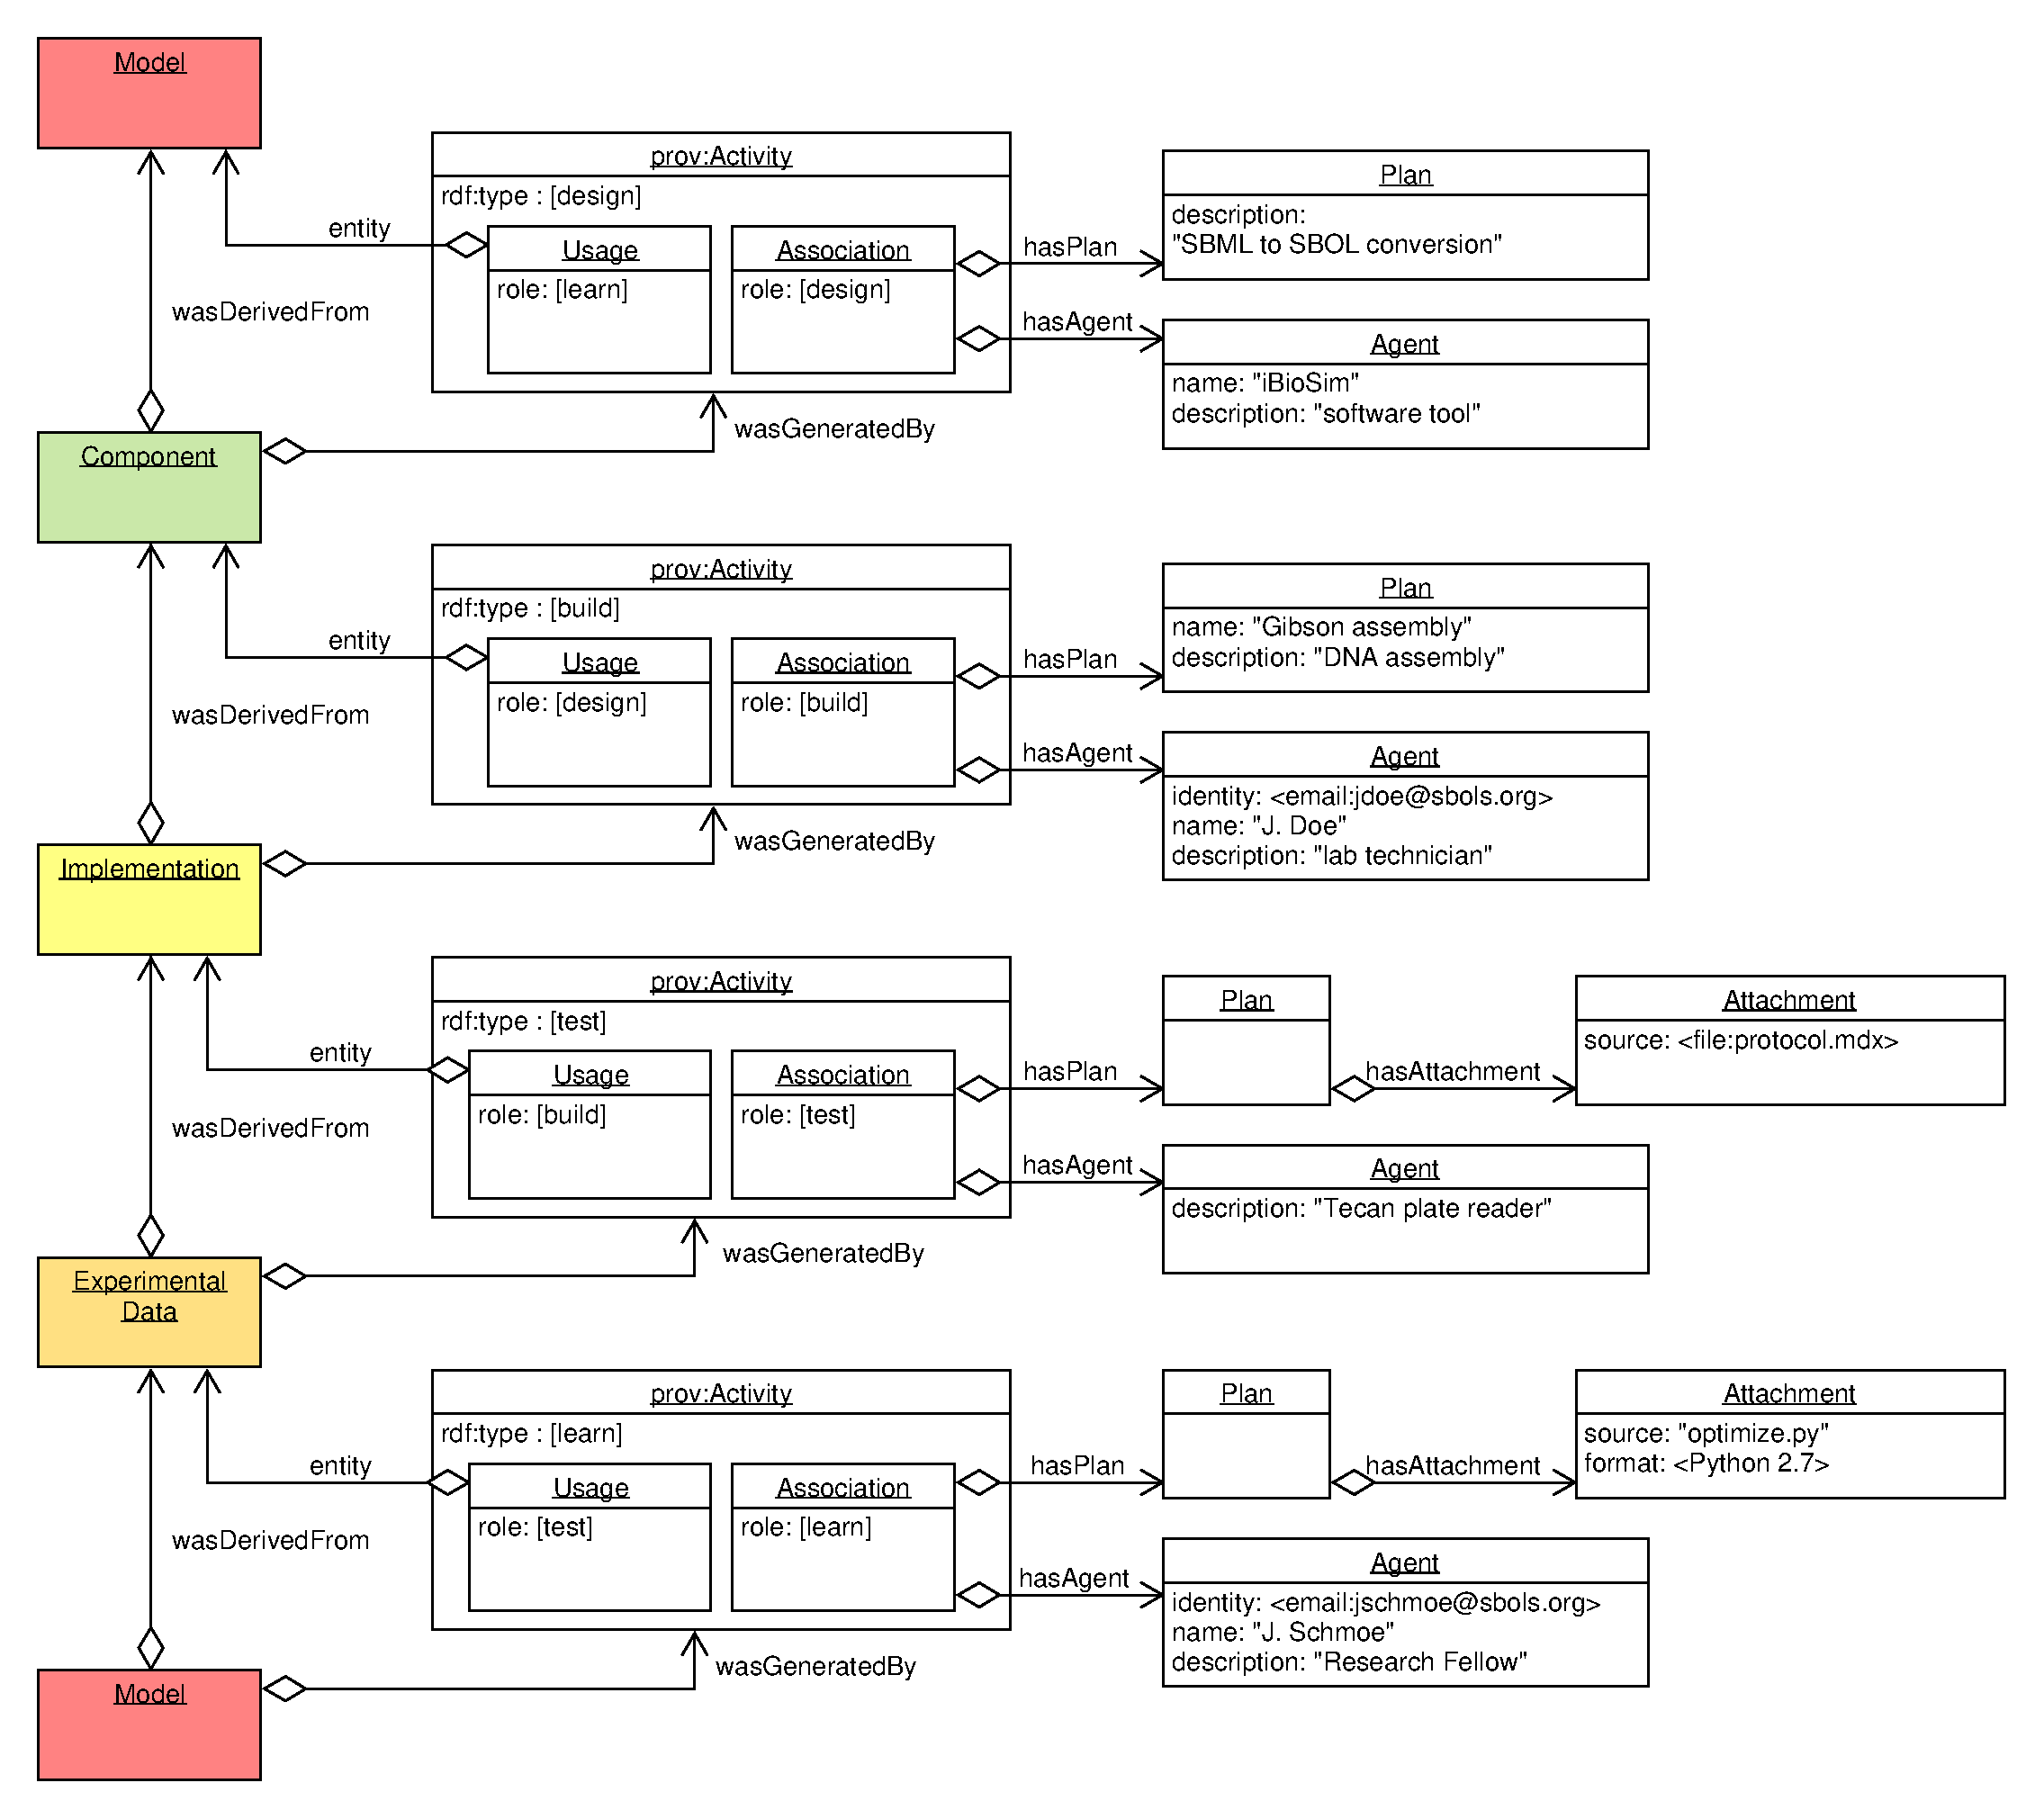
\includegraphics[width=0.75\linewidth]{uml/design-build-test}
\caption[]{An example data structure representing an idealized workflow for model-based design.}
\label{images:design-build-test-learn}
\end{center}
\end{figure}

%% proposed by issue #137
\clearpage

\subparagraph{Example - Combinatorial Derivation}

As specified in the description of \sbol{CombinatorialDerivation}, provenance can be used to link each generated \sbol{Component} (or \sbol{Collection} thereof) back to the source form which it was derived.
In particular, each derived design links with \prov{wasDerivedFrom} to the \sbol{CombinatorialDerivation} that it was derived from.  Also, each \sbol{SubComponent} has a \prov{wasDerivedFrom} linking it to the \sbol{SubComponent} within the \sbol{template} that it is derived from.  The advantage of these provenance links is that they provide sufficient information to validate that this derived design has been properly derived from the specified \sbol{CombinatorialDerivation}s.

\subsection{Adding Measures/Parameters with OM}
\label{sec:parameters}

There are at least two well-established cases for including measures/parameters and their associated units in SBOL design specifications. These use cases are the specification of genetic circuit designs and their associated parameters (such as rates of transcription) and the specification of environmental conditions for biological system designs (such as growth media concentrations and temperatures). In the first use case, parameters are necessary to enable the generation of quantitive models of circuit behavior from circuit design specifications. In the second use case, measures are necessary to define experimental conditions and enable the analysis of system behavior or characterization with respect to environmental context.

The Ontology of Units of Measure (OM) (\url{http://www.ontology-of-units-of-measure.org/resource/om-2}) already defines a data model for representing measures and their associated units. Here, a subset of OM is adopted by SBOL to describe these concepts for biological design specifications. As shown in \ref{uml:om}, SBOL leverages three of the base classes defined by the OM: \om{Measure}, \om{Unit} and \om{Prefix}. A \om{Measure} links a numerical value to a \om{Unit}, which may or may not have a \om{Prefix} (e.g. centi, milli, micro, etc.). As these classes are adopted by SBOL, \om{Measure} is treated as a subclass of \sbol{Identified}, while \om{Unit} and \om{Prefix} are treated as subclasses of \sbol{TopLevel}. In addition, SBOL adopts the following OM \om{Unit} subclasses: \om{SingularUnit}, \om{CompoundUnit}, \om{UnitMultiplication}, \om{UnitDivision}, \om{UnitExponentiation}, and \om{PrefixedUnit}. Lastly, SBOL adopts the following \om{Prefix} subclasses from OM: \om{SIPrefix} and \om{BinaryPrefix}.

\begin{figure}[ht]
\begin{center}
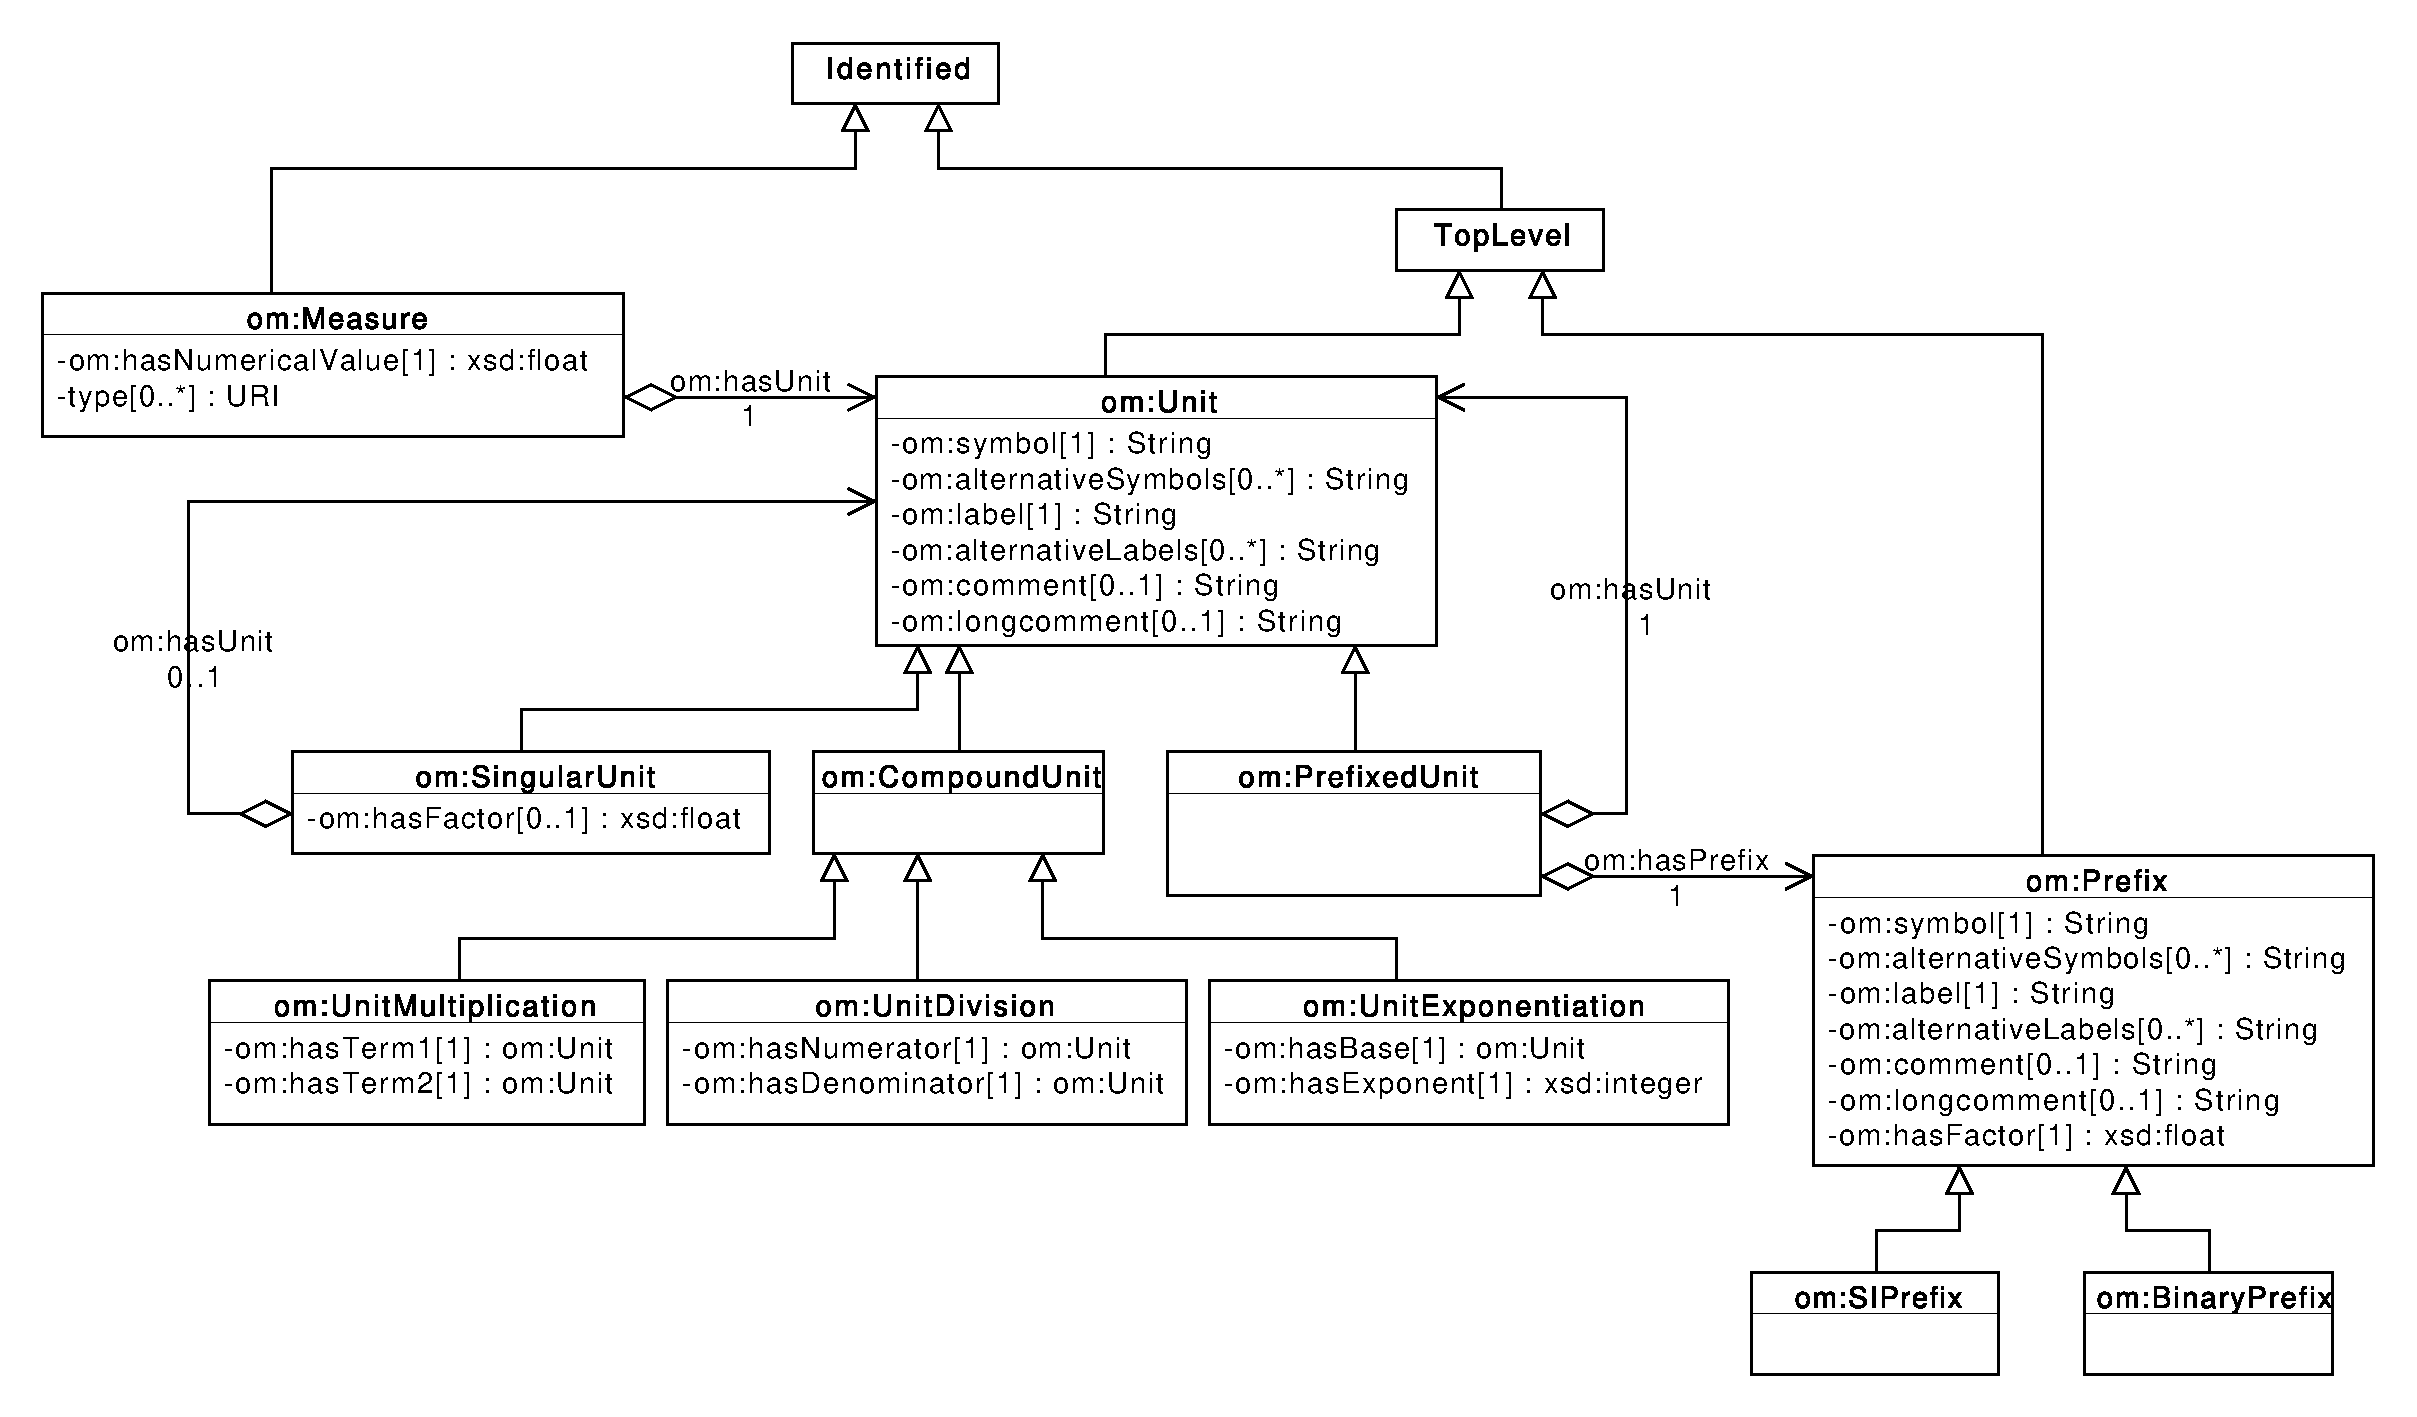
\includegraphics[width=\linewidth]{uml/om}
\caption[]{OM classes adopted by SBOL and their subclass relationships to \sbol{Identified} and \sbol{TopLevel}}
\label{uml:om}
\end{center}
\end{figure}

SBOL-compliant tools are allowed to read, write, and modify data belonging to OM classes other than those described here, but this specification does not provide any guidance for the interpretation or use of these data in the context of SBOL.

\subsubsection{om:Measure} \label{sec:om:Measure}

The purpose of the \om{Measure} class is to link a numerical value to a \om{Unit}. 

\subparagraph{The \sbolheading{om:hasNumericalValue} property}\label{sec:om:hasNumericalValue}
The \om{hasNumericalValue} property is REQUIRED and MUST contain a single xsd:float.

\subparagraph{The \sbolheading{om:hasUnit} property}\label{sec:om:hasUnit:Measure}
The \ommult{hasUnit:Measure}{hasUnit} property is REQUIRED and MUST contain a \sbol{URI} that refers to a \om{Unit}. The OM provides \sbol{URI}s for many existing instances of the \om{Unit} class for reference (for example,\\ \url{http://www.ontology-of-units-of-measure.org/resource/om-2/gramPerLitre}).

\subparagraph{The \sbolheading{type} property}\label{sec:type:Measure}

A \om{Measure} MAY have one or more \sbolmult{type:Measure}{type} properties, each is of type \sbol{URI}. It is RECOMMENDED that one of these \sbol{URI}s identify a term from the Systems Description Parameter branch of the Systems Biology Ontology (SBO) (\url{http://www.ebi.ac.uk/sbo/main/}). This \sbolmult{type:Measure}{type} property of the \om{Measure} class is not specified in the OM and is added by SBOL to describe different types of parameters 
(for example, rate of reaction is identified by the SBO term \url{http://identifiers.org/SBO:0000612}).

\subsubsection{om:Unit}
\label{sec:om:Unit}

As adopted by SBOL, \om{Unit} is an abstract class that is extended by other classes to describe units of measure using a shared set of properties. 

\subparagraph{The \sbolheading{om:symbol} property}\label{sec:om:symbol:Unit}
The \ommult{symbol:Unit}{symbol} property is REQUIRED and MUST contain a \sbol{String}. This \sbol{String} is commonly used to abbreviate the unit of measure's name. For example, the unit of measure named ``gram per liter'' is commonly abbreviated using the \sbol{String} ``g/l''.

\subparagraph{The \sbolheading{om:alternativeSymbols} property}\label{sec:om:alternativeSymbols:Unit}
The \ommult{alternativeSymbols:Unit}{alternativeSymbols} property is OPTIONAL and MAY contain a set of \sbol{String}s. This property can be used to specify alternative abbreviations other than that specified using the \ommult{symbol:Unit}{symbol} property.

\subparagraph{The \sbolheading{om:label} property}\label{sec:om:label:Unit}
The \ommult{label:Unit}{label} property is REQUIRED and MUST contain a \sbol{String}. This \sbol{String} is a common name for the unit of measure and SHOULD be identical to any \sbol{String} contained by the \sbol{name} property inherited from \sbol{Identified}.

\subparagraph{The \sbolheading{om:alternativeLabels} property}\label{sec:om:alternativeLabels:Unit}
The \ommult{alternativeLabels:Unit}{alternativeLabels} property is OPTIONAL and MAY contain a set of \sbol{String}s. This property can be used to specify alternative common names other than that specified using the \ommult{label:Unit}{label} property.

\subparagraph{The \sbolheading{om:comment} property}\label{sec:om:comment:Unit}
The \ommult{comment:Unit}{comment} property is OPTIONAL and MAY contain a \sbol{String}. This \sbol{String} is a description of the unit of measure and SHOULD be identical to any \sbol{String} contained by the \sbol{description} property inherited from \sbol{Identified}.

\subparagraph{The \sbolheading{om:longcomment} property}\label{sec:om:longcomment:Unit}
The \ommult{longcomment:Unit}{longcomment} property is OPTIONAL and MAY contain a \sbol{String}. This \sbol{String} is a long description of the unit of measure and SHOULD be longer than any \sbol{String} contained by the \ommult{comment:Unit}{comment} property.

\subsubsection{om:SingularUnit}
\label{sec:om:SingularUnit}

The purpose of the \om{SingularUnit} class is to describe a unit of measure that is not explicitly represented as a combination of multiple units, but could be equivalent to such a representation. For example, a joule is considered to be a \om{SingularUnit}, but it is equivalent to the multiplication of a newton and a meter.  

\subparagraph{The \sbolheading{om:hasUnit} property}\label{sec:om:hasUnit:SingularUnit}
The \ommult{hasUnit:SingularUnit}{hasUnit} is OPTIONAL and MAY contain a \sbol{URI}. This \sbol{URI} MUST refer to another \om{Unit}. The \ommult{hasUnit:SingularUnit}{hasUnit} propery can be used in conjunction with the \ommult{hasFactor:SingularUnit}{hasFactor} property to specify whether a \om{SingularUnit} is equivalent to another \om{Unit} multiplied by a factor. For example, an angstrom is equivalent to $10^{-10}$ meters.

\subparagraph{The \sbolheading{om:hasFactor} property}\label{sec:om:hasFactor:SingularUnit}
The \ommult{hasFactor:SingularUnit}{hasFactor} property is OPTIONAL and MAY contain a xsd:float. If the \ommult{hasFactor:SingularUnit}{hasFactor} property of a \om{SingularUnit} is non-empty, then its \ommult{hasUnit:SingularUnit}{hasUnit} property SHOULD also be non-empty.

\subsubsection{om:CompoundUnit}
\label{sec:om:CompoundUnit}

As adopted by SBOL, \om{CompoundUnit} is an abstract class that is extended by other classes to describe units of measure that can be represented as combinations of multiple other units of measure.

\subsubsection{om:UnitMultiplication}
\label{sec:om:UnitMultiplication}

The purpose of the \om{UnitMultiplication} class is to describe a unit of measure that is the multiplication of two other units of measure. 

\subparagraph{The \sbolheading{om:hasTerm1} property}\label{sec:om:hasTerm1}
The \om{hasTerm1} property is REQUIRED and MUST contain a \sbol{URI} that refers to another \om{Unit}. This \om{Unit} is the first multiplication term.

\subparagraph{The \sbolheading{om:hasTerm2} property}\label{sec:om:hasTerm2}
The \om{hasTerm2} property is REQUIRED and MUST contain a \sbol{URI} that refers to another \om{Unit}. This \om{Unit} is the second multiplication term. It is okay if the \om{Unit} referred to by \om{hasTerm1} is the same as that referred to by \om{hasTerm2}.

\subsubsection{om:UnitDivision}
\label{sec:om:UnitDivision}

The purpose of the \om{UnitDivision} class is to describe a unit of measure that is the division of one unit of measure by another.

\subparagraph{The \sbolheading{om:hasNumerator} property}\label{sec:om:hasNumerator}
The \om{hasNumerator} property is REQUIRED and MUST contain a \sbol{URI} that refers to another \om{Unit}.

\subparagraph{The \sbolheading{om:hasDenominator} property}\label{sec:om:hasDenominator}
The \om{hasDenominator} property is REQUIRED and MUST contain a \sbol{URI} that refers to another \om{Unit}.

\subsubsection{om:UnitExponentiation}
\label{sec:om:UnitExponentiation}

The purpose of the \om{UnitExponentiation} class is to describe a unit of measure that is raised to an integer power.

\subparagraph{The \sbolheading{om:hasBase} property}\label{sec:om:hasBase}
The \om{hasBase} property is REQUIRED and MUST contain a \sbol{URI} that refers to another \om{Unit}.

\subparagraph{The \sbolheading{om:hasExponent} property}\label{sec:om:hasExponent}
The \om{hasExponent} property is REQUIRED and MUST contain an \texttt{xsd:integer}.

\subsubsection{om:PrefixedUnit}
\label{sec:om:PrefixedUnit}

The purpose of the \om{PrefixedUnit} class is to describe a unit of measure that is the multiplication of another unit of measure and a factor represented by a standard prefix such as ``milli,'' ``centi,'' ``kilo,'' etc. 

\subparagraph{The \sbolheading{om:hasUnit} property}\label{sec:om:hasUnit:PrefixedUnit}
The \ommult{hasUnit:PrefixedUnit}{hasUnit} property is REQUIRED and MUST contain a \sbol{URI} that refers to another \om{Unit}. 

\subparagraph{The \sbolheading{om:hasPrefix} property}\label{sec:om:hasPrefix}
The \om{hasPrefix} property is REQUIRED and MUST contain a \sbol{URI} that refers to a \om{Prefix}.

\subsubsection{om:Prefix}
\label{sec:om:Prefix}

As adopted by SBOL, \om{Prefix} is an abstract class that is extended by other classes to describe factors that are commonly represented by standard unit prefixes. For example, the factor $10^{-3}$ is represented by the standard unit prefix ``milli.'' 

\subparagraph{The \sbolheading{om:symbol} property}\label{sec:om:symbol:Prefix}
The \ommult{symbol:Prefix}{symbol} property is REQUIRED and MUST contain a \sbol{String}. This \sbol{String} is commonly used to abbreviate the name of the unit prefix. For example, the \sbol{String} ``m'' is commonly used to abbreviate the name ``milli.''

\subparagraph{The \sbolheading{om:alternativeSymbols} property}\label{sec:om:alternativeSymbols:Prefix}
The \ommult{alternativeSymbols:Prefix}{alternativeSymbols} property is OPTIONAL and MAY contain a set of \sbol{String}s. This property can be used to specify alternative abbreviations other than that specified using the \ommult{symbol:Prefix}{symbol} property.

\subparagraph{The \sbolheading{om:label} property}\label{sec:om:label:Prefix}
The \ommult{label:Prefix}{label} property is REQUIRED and MUST contain a \sbol{String}. This \sbol{String} is a common name for the unit prefix and SHOULD be identical to any \sbol{String} contained by the \sbol{name} property inherited from \sbol{Identified}.

\subparagraph{The \sbolheading{om:alternativeLabels} property}\label{sec:om:alternativeLabels:Prefix}
The \ommult{alternativeLabels:Prefix}{alternativeLabels} property is OPTIONAL and MAY contain a set of \sbol{String}s. This property can be used to specify alternative common names other than that specified using the \ommult{label:Prefix}{label} property.

\subparagraph{The \sbolheading{om:comment} property}\label{sec:om:comment:Prefix}
The \ommult{comment:Prefix}{comment} property is OPTIONAL and MAY contain a \sbol{String}. This \sbol{String} is a description of the unit prefix and SHOULD be identical to any \sbol{String} contained by the \sbol{description} property inherited from \sbol{Identified}.

\subparagraph{The \sbolheading{om:longcomment} property}\label{sec:om:longcomment:Prefix}
The \ommult{longcomment:Prefix}{longcomment} property is OPTIONAL and MAY contain a \sbol{String}. This \sbol{String} is a long description of the unit of measure and SHOULD be longer than any \sbol{String} contained by the \ommult{comment:Prefix}{comment} property.

\subparagraph{The \sbolheading{om:hasFactor} property}\label{sec:om:hasFactor:Prefix}
The \ommult{hasFactor:Prefix}{hasFactor} property is REQUIRED and MUST contain an xsd:float.

\subsubsection{om:SIPrefix}
\label{sec:om:SIPrefix}

The purpose of the \om{SIPrefix} class is to describe standard SI prefixes such as ``milli,'' ``centi,'' ``kilo,'' etc. 

\subsubsection{om:BinaryPrefix}
\label{sec:om:BinaryPrefix}

The purpose of the \om{BinaryPrefix} class is to describe standard binary prefixes such as ``kibi,'' ``mebi,'' ``gibi,'' etc. These prefixes commonly precede units of information such as ``bit'' and ``byte.''

\begin{figure}[ht]
\begin{center}
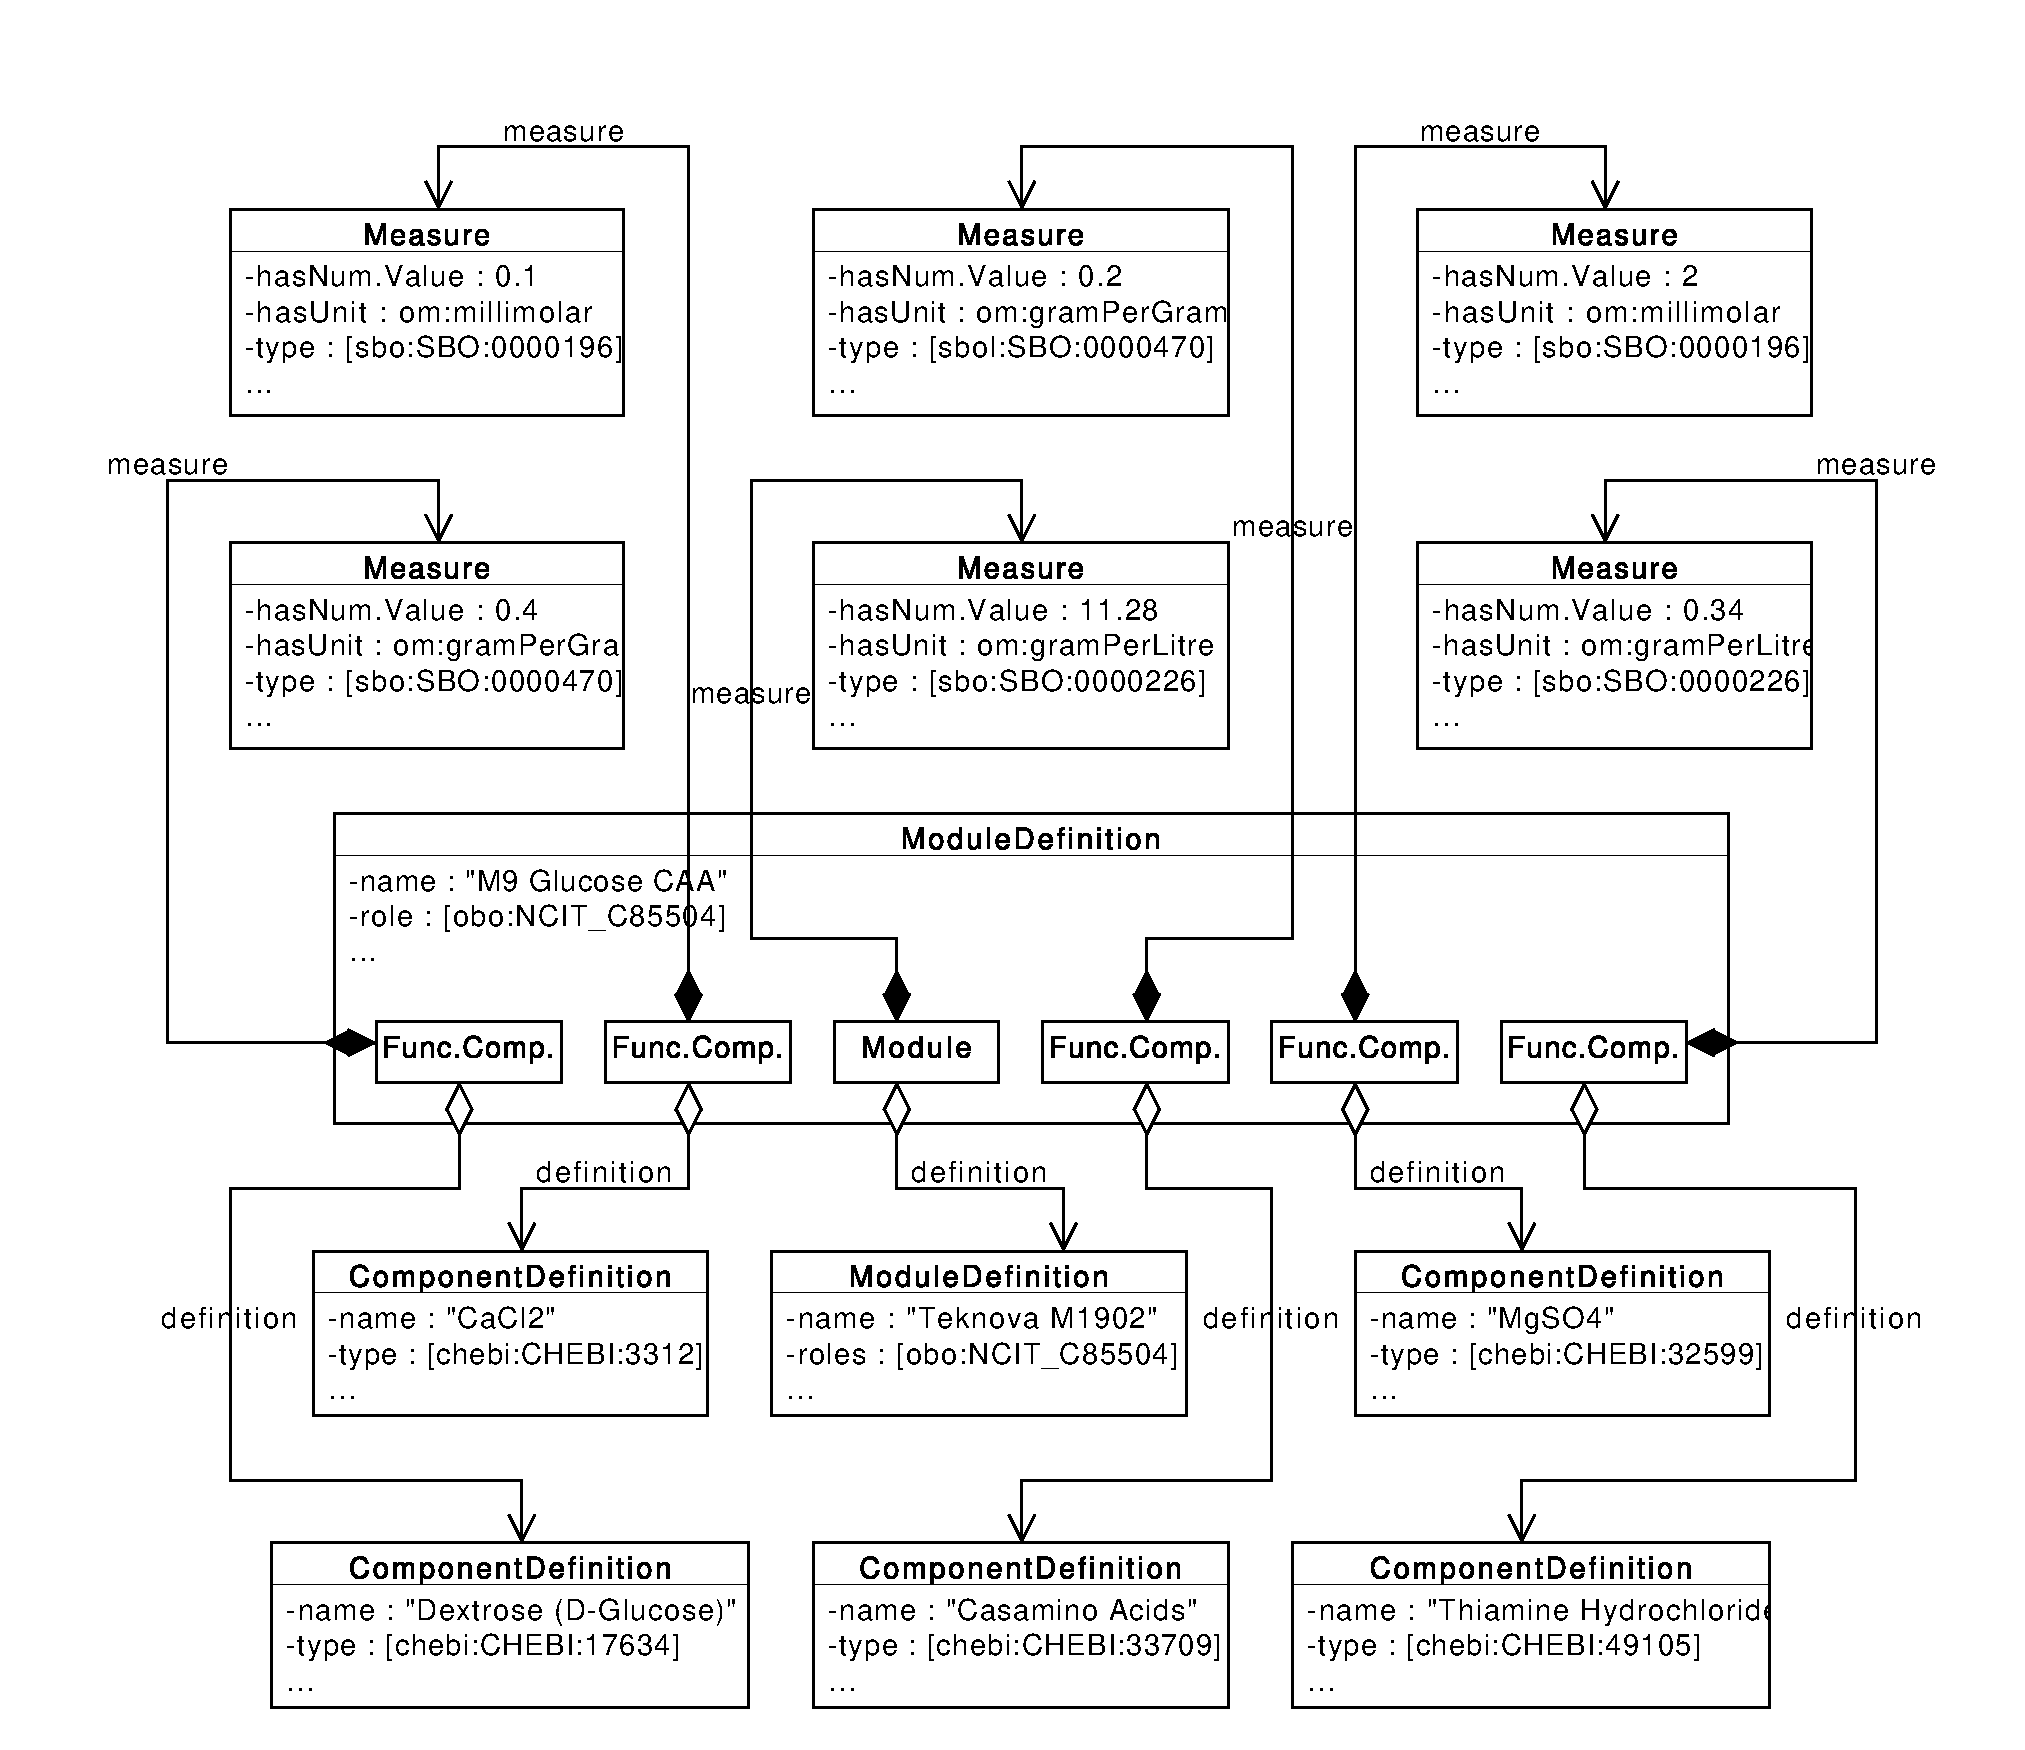
\includegraphics[width=\linewidth]{uml/media_example}
\caption[]{Growth media recipe represented using instances of the \om{Measure} and \om{Unit} classes from the OM.}
\label{uml:media_example}
\end{center}
\end{figure}


\newcounter{sbolCtr}
\newcommand{\printValid}{\validRule{sbol-\arabic{sbolCtr}\addtocounter{sbolCtr}{1}}}
\newcommand{\printWarning}{\consistencyRule{sbol-\arabic{sbolCtr}\addtocounter{sbolCtr}{1}}}
\newcommand{\printModeling}{\modelingRule{sbol-\arabic{sbolCtr}\addtocounter{sbolCtr}{1}}}

\section{Validation Rules}
\label{validation}

This section summarizes all the conditions that MUST be or 
are RECOMMENDED to be true of an SBOL Version~2 document.  
There are different degrees of rule strictness.  
Rules of the former kind are strict SBOL validation rules---data encoded in SBOL MUST conform to
all of them in order to be considered valid.  Rules of the latter kind
are consistency rules that are RECCOMENDED for following best practices.  To help highlight these differences, we use the
following symbols next to the rule numbers:

\begin{description}

\item[\hspace*{6.5pt}\vSymbol\vsp] A \vSymbolName indicates a strong
  REQUIRED condition for SBOL conformance. If a SBOL document does not follow this rule, it does not conform to the SBOL
  specification.  (Mnemonic intention behind the choice of symbol:
  ``This must be checked.'')

\item[\hspace*{6.5pt}\cSymbol\csp] A \cSymbolName indicates a weak
  REQUIRED condition for SBOL conformance. While this rule MUST be followed, it is difficult, if not  impossible, for a machine to automatically check whether the rule has been followed. (Mnemonic intention behind the choice of symbol: ``This is a cause for warning.'')

\item[\hspace*{6.5pt}\mSymbol\msp] A \mSymbolName indicates a 
  RECOMMENDED condition for following best practices.  This rule is not strictly a matter of SBOL conformance, but its recommendation comes from logical
  reasoning.  If an SBOL document does not follow this rule, it is still valid SBOL, but it may have degraded functionality in some tools.  (Mnemonic intention behind the choice of symbol: ``You're a star if you heed this.'')

\end{description}

The validation rules listed in the following subsections should all be
stated or implied in the rest of this specification document.  They
are enumerated here for convenience and to provide a ``master
checklist'' for SBOL compliance.  In case of a conflict between this
section and other portions of the specification (though there should
be none), this section is considered authoritative for purpose of
determining SBOL document compliance.

For \notice convenience and brievity, we use the shorthand
``\token{sbol:x}'' to stand for an attribute or element name \token{x}
in the namespace for the SBOL specification, using
the namespace prefix \token{sbol}.  In reality, the prefix string may be different from the literal ``\token{sbol}'' used here (and indeed, it can be any valid XML namespace prefix that the software
chooses).  We use ``\token{sbol:x}'' because it is shorter than to
write a full explanation everywhere we refer to an attribute or element
in the SBOL specification namespace.

\subsubsection*{General rules about an SBOL document}
\setcounter{sbolCtr}{10101} 

\printValid{An SBOL document MUST declare the use of the following XML namespace: \\ \textls[-25]{\uri{http://sbols.org/v2\#}}.\\
Reference: \sec{xml-namespace}}

\printValid{An SBOL document MUST declare the use of the following XML namespace: \\ \textls[-25]{\uri{http://www.w3.org/1999/02/22-rdf-syntax-ns\#}}.\\
Reference: \sec{xml-namespace}}

\printValid{An SBOL document MUST declare the use of the following XML namespace when it includes any \sbol{name} or \sbol{description} properties: \\ \textls[-25]{\uri{http://purl.org/dc/terms/}}.\\ 
Reference: \sec{xml-namespace}}

\printValid{An SBOL document MUST declare the use of the following XML namespace when it includes any \sbol{wasDerivedFrom} properties: \\ \textls[-25]{\uri{http://www.w3.org/ns/prov\#}}.\\ Reference: \sec{xml-namespace}}

\subsubsection*{Rules for the \class{Identified} class} 
\setcounter{sbolCtr}{10201}

\printValid{The \sbol{identity} is a REQUIRED property for all \sbol{Identified} objects and has a data type of URI with a syntax defined by:\\
\uri{http://www.w3.org/1999/02/22-rdf-syntax\#about} \\ 
Reference: \sec{sec:Identified}}

\printValid{The \sbol{persistentIdentity} is an OPTIONAL property for all \sbol{Identified} objects and, if provided, has a data type of \sbol{URI} with a syntax defined by:\\ \uri{http://www.w3.org/1999/02/22-rdf-syntax\#about}\\ 
Reference: \sec{sec:Identified}}

\printValid{The \sbol{displayId} is an OPTIONAL property for all \sbol{Identified} objects and, if provided, has a data type of String that is composed only of alphanumeric or underscore characters and MUST NOT begin with a digit.\\ Reference: \sec{sec:Identified}}

\printValid{The \sbol{version} is an OPTIONAL property for all \sbol{Identified} objects and, if provided, has a data type of String that is composed only of alphanumeric characters, underscores, hyphens, and periods and MUST begin with a digit.\\ Reference: \sec{sec:Identified}}

\printValid{The \sbol{annotations} field is an OPTIONAL list of for all \sbol{Identified} objects and, if provided, includes references to \sbol{Annotation} objects.\\ Reference: \sec{sec:Identified}}

\printValid{The \sbol{wasDerivedFrom} property is OPTIONAL for all \sbol{Identified} objects and, if provided, has a data type of \sbol{URI}.  \\ Reference: \sec{sec:Identified}}

\printValid{The \sbol{name} is an OPTIONAL property for all \sbol{Identified} objects and, if provided, has a data type of String.  \\ Reference: \sec{sec:Identified}}

\printValid{The \sbol{description} is an OPTIONAL property for all \sbol{Identified} objects and, if provided, has a data type of String.  \\ Reference: \sec{sec:Identified}}

\printModeling{The \sbol{displayId} of a compliant object is REQUIRED.  \\ Reference: \sec{sec:compliant}}

\printModeling{The \sbol{persistentIdentity} of a compliant top level object is REQUIRED and MUST end with a delimiter ('/', '\#', or ':') followed by the \sbol{displayId} of the object.\\ Reference: \sec{sec:compliant}}

\printModeling{The \sbol{persistentIdentity} of a compliant child object is REQUIRED and MUST begin with the\\ \sbol{persistentIdentity} of its parent object and be immediately followed by a delimiter ('/', '\#', or ':') and the \sbol{displayId} of the object.\\ Reference: \sec{sec:compliant}}

\printModeling{The \sbol{identity} of a compliant object MUST either be equal to the \sbol{persistentIdentity} when no \sbol{version} is specified or equal to "\refObj{persistentIdentity}/\refObj{version}" when a \sbol{version} is provided.\\ Reference: \sec{sec:compliant}}

\printModeling{The \sbol{version} of a compliant child object is REQUIRED to be equal to the \sbol{version} of its parent object.\\ Reference: \sec{sec:compliant}}

\subsubsection*{Rules for the \class{TopLevel} class} 
\setcounter{sbolCtr}{10301}

\printValid{A \sbol{TopLevel} object inherits all properties of a \sbol{Identified} object.\\ Reference: \sec{sec:TopLevel}}

\subsubsection*{Rules for the \class{Sequence} class} 
\setcounter{sbolCtr}{10401}

\printValid{A \sbol{Sequence} MUST inherit all properties of the \sbol{TopLevel} class.\\ Reference: \sec{sec:Sequence}}

\printValid{The \sbol{elements} property of a \sbol{Sequence} is REQUIRED and MUST contain a \external{String}.\\ Reference: \sec{sec:Sequence}}

\printValid{The \sbol{encoding} property of \sbol{Sequence} is REQUIRED and MUST contain a \external{URI}.\\ Reference: \sec{sec:Sequence}}

\printWarning{The \sbol{encoding} property of a \sbol{Sequence} MUST contain a \external{URI} from \ref{tbl:sequence_encodings} if it is well-described by this \external{URI}.\\ Reference: \sec{sec:Sequence}}

\printWarning{The \sbol{elements} property of a \sbol{Sequence} MUST be consistent with its \sbol{encoding} property.\\ Reference: \sec{sec:Sequence}}

\subsubsection*{Rules for the \class{ComponentDefinition} class} 
\setcounter{sbolCtr}{10501}

\printValid{A \sbol{ComponentDefinition} MUST inherit all properties of the \sbol{TopLevel} class.\\ Reference: \sec{sec:ComponentDefinition}}

\printValid{The \sbolmult{types:CD}{types} property of a \sbol{ComponentDefinition} is REQUIRED and MUST contain a non-empty set of \external{URI}s.\\ Reference: \sec{sec:ComponentDefinition}}

\printValid{The \sbolmult{types:CD}{types} property of a \sbol{ComponentDefinition} MUST NOT contain more than one \external{URI} from \ref{tbl:componentdefinition_types}.\\ Reference: \sec{sec:ComponentDefinition}}

\printWarning{The \sbolmult{types:CD}{types} property of a \sbol{ComponentDefinition} MUST contain a \external{URI} from \ref{tbl:componentdefinition_types} if it is well-described by this \external{URI}.\\ Reference: \sec{sec:ComponentDefinition}}

\printWarning{Each \external{URI} contained by the \sbolmult{types:CD}{types} property of a \sbol{ComponentDefinition} MUST refer to an ontology term that describes the category of biochemical or physical entity that is represented by the \sbol{ComponentDefinition}.\\ Reference: \sec{sec:ComponentDefinition}}

\printWarning{All \external{URI}s contained by the \sbolmult{types:CD}{types} property of a \sbol{ComponentDefinition} MUST refer to non-conflicting ontology terms.\\ Reference: \sec{sec:ComponentDefinition}}

\printValid{The \sbolmult{roles:CD}{roles} property of a \sbol{ComponentDefinition} is OPTIONAL and MAY contain a set of \external{URI}s.\\ Reference: \sec{sec:ComponentDefinition}}

\printWarning{The \sbolmult{roles:CD}{roles} property of a \sbol{ComponentDefinition} MUST contain a \external{URI} from \ref{tbl:componentdefinition_roles} if it is well-described by this \external{URI}.\\ Reference: \sec{sec:ComponentDefinition}}

\printWarning{Each \external{URI} contained by the \sbolmult{roles:CD}{roles} property of a \sbol{ComponentDefinition} MUST refer to an ontology term that clarifies the potential function of the \sbol{ComponentDefinition} in a biochemical or physical context.\\ Reference: \sec{sec:ComponentDefinition}}

\printWarning{Each \external{URI} contained by the \sbolmult{roles:CD}{roles} property of a \sbol{ComponentDefinition} MUST refer to an ontology term that is consistent with its \sbolmult{types:CD}{types} property.\\ Reference: \sec{sec:ComponentDefinition}}

\printModeling{The \sbolmult{roles:CD}{roles} property of a  \sbol{ComponentDefinition} SHOULD only contain a \external{URI} provided in  \ref{tbl:componentdefinition_roles} if one of its \sbolmult{types:CD}{types} is cross-listed with the \external{URI}.\\ Reference: \sec{sec:ComponentDefinition}}

\printValid{The \sbol{sequences} property of a \sbol{ComponentDefinition} is OPTIONAL and MAY contain a set of \external{URI} references to \sbol{Sequence} objects.\\ Reference: \sec{sec:ComponentDefinition}}

\printWarning{Each \external{URI} in the set of \sbol{sequences} MUST reference a \sbol{Sequence} object.\\ Reference: \sec{sec:ComponentDefinition}}

\printWarning{The \sbol{sequences} property of a \sbol{ComponentDefinition} MUST NOT refer to \sbol{Sequence} objects with conflicting \sbol{encoding} properties.\\ Reference: \sec{sec:ComponentDefinition}}

\printWarning{The \sbol{Sequence} objects referred to by the \sbol{sequences} property of a \sbol{ComponentDefinition} MUST be consistent with each other, such that well-defined mappings exist between their \sbol{elements} properties in accordance with their \sbol{encoding} properties.\\ Reference: \sec{sec:ComponentDefinition}}

\printWarning{The \sbol{sequences} property of a \sbol{ComponentDefinition} MUST NOT refer to \sbol{Sequence} objects with conflicting \external{IUPAC} \sbol{encoding} \external{URI}s from \ref{tbl:sequence_encodings}.\\ Reference: \sec{sec:ComponentDefinition}}

\printWarning{If the \sbol{sequences} property of a \sbol{ComponentDefinition} refers to one or more \sbol{Sequence} objects, and one of the  \sbolmult{types:CD}{types} of this \sbol{ComponentDefinition} comes from \ref{tbl:componentdefinition_types}, then one of the \sbol{Sequence} objects MUST have the \sbol{encoding} that is cross-listed with this type in \ref{tbl:sequence_encodings}.\\ Reference: \sec{sec:ComponentDefinition}}

\printWarning{If the \sbol{sequences} property of a \sbol{ComponentDefinition} refers to a \sbol{Sequence} with an \sbol{encoding} from \ref{tbl:sequence_encodings}, then the \sbolmult{types:CD}{types} property of the \sbol{ComponentDefinition} MUST contain the type from \ref{tbl:componentdefinition_types} that is cross-listed with this \sbol{encoding} in  \ref{tbl:sequence_encodings}.\\ Reference: \sec{sec:ComponentDefinition}}

\printModeling{If a \sbol{ComponentDefinition} refers to more than one \sbol{Sequence} with the same \sbol{encoding}, then the \sbol{elements} of these \sbol{Sequence} objects SHOULD have equal lengths.\\ Reference: \sec{sec:ComponentDefinition}}

\printValid{The \sbol{components} property of a \sbol{ComponentDefinition} is OPTIONAL and MAY contain a set of \sbol{Component} objects.\\ Reference: \sec{sec:ComponentDefinition}}

\printModeling{If a \sbol{ComponentDefinition} in a \sbol{ComponentDefinition}-\sbol{Component} hierarchy refers to one or more \sbol{Sequence} objects, and there exist \sbol{ComponentDefinition} objects lower in the hierarchy that refer to \sbol{Sequence} objects with the same \sbol{encoding}, then the \sbol{elements} properties of these \sbol{Sequence} objects SHOULD be consistent with each other, such that well-defined mappings exist from the ``lower level'' \sbol{elements} to the ``higher level'' \sbol{elements} in accordance with their shared \sbol{encoding} (subject to any restrictions on the positions of \sbol{Component} objects in the hierarchy that are imposed by \sbol{SequenceAnnotation} or \sbol{SequenceConstraint} objects).\\ Reference: \sec{sec:ComponentDefinition}}

\printValid{The \sbol{sequenceAnnotations} property of a \sbol{ComponentDefinition} is OPTIONAL and MAY contain a set of \sbol{SequenceAnnotation} objects.\\ Reference: \sec{sec:ComponentDefinition}}

\printValid{If the \sbol{sequenceAnnotations} property of a \sbol{ComponentDefinition} must not contain two or more \sbol{SequenceAnnotation} objects that refer to the same \sbol{Component}.\\ Reference: \sec{sec:ComponentDefinition}}

\printModeling{If the \sbol{sequences} property of a \sbol{ComponentDefinition} refers to a \sbol{Sequence} with an \external{IUPAC} \sbol{encoding} from \ref{tbl:sequence_encodings}, then each \sbol{SequenceAnnotation} that includes a \sbol{Range} and/or \sbol{Cut} in the \sbol{sequenceAnnotations} property of the \sbol{ComponentDefinition} SHOULD specify a region on the \sbol{elements} of this \sbol{Sequence}.\\ Reference: \sec{sec:ComponentDefinition}}

\printValid{The \sbol{sequenceConstraints} property of a \sbol{ComponentDefinition} is OPTIONAL and MAY contain a set of \sbol{SequenceConstraint} objects.  \\ Reference: \sec{sec:ComponentDefinition}}

\subsubsection*{Rules for the \class{ComponentInstance} class} 
\setcounter{sbolCtr}{10601}

\printValid{A \sbol{ComponentInstance} MUST inherit all properties of the \sbol{Identified} class.\\ Reference: \sec{sec:ComponentInstance}}

\printValid{The \sbol{access} property of a \sbol{ComponentInstance} is REQUIRED and MUST contain a \external{URI} from \ref{tbl:componentInstance_access} \\ Reference: \sec{sec:ComponentInstance}}

\printValid{The \sbolmult{definition:CI}{definition} property of a \sbol{ComponentInstance} is REQUIRED and MUST contain a \external{URI} reference to a \sbol{ComponentDefinition}.\\ Reference: \sec{sec:ComponentInstance}}

\printWarning{The \sbol{definition} property \external{URI} must reference a \sbol{ComponentDefinition} object.\\ Reference: \sec{sec:ComponentInstance}}

\printValid{The \sbolmult{definition:CI}{definition} property of a \sbol{ComponentInstance} MUST NOT contain a \external{URI} reference to the \sbol{ComponentDefinition} that contains the \sbol{ComponentInstance}.\\ Reference: \sec{sec:ComponentInstance}}

\printWarning{\sbol{ComponentInstance} objects MUST NOT form circular reference chains via their \sbolmult{definition:CI}{definition} properties and parent \sbol{ComponentDefinition} objects.\\ Reference: \sec{sec:ComponentInstance}}

\printValid{The \sbolmult{mapsTos:CI}{mapsTos} property of a \sbol{ComponentInstance} is OPTIONAL and MAY contain a set of \sbol{MapsTo} objects.\\ Reference: \sec{sec:ComponentInstance}}

\subsubsection*{Rules for the \class{Component} class} 
\setcounter{sbolCtr}{10701}

\printValid{A \sbol{Component} MUST inherit all properties of the \sbol{ComponentInstance} class.\\ Reference: \sec{sec:ComponentInstance}}

\subsubsection*{Rules for the \class{MapsTo} class} 
\setcounter{sbolCtr}{10801}

\printValid{A \sbol{MapsTo} MUST inherit all properties of the \sbol{Identified} class.\\ Reference: \sec{sec:MapsTo}}

\printValid{The \sbol{local} property of a \sbol{MapsTo} is REQUIRED and MUST contain a \external{URI} reference to a \sbol{ComponentInstance}.\\ Reference: \sec{sec:MapsTo}}

\printValid{If a \sbol{MapsTo} is contained by a \sbol{Component} in a \sbol{ComponentDefinition}, then the \sbol{local} property of the \sbol{MapsTo} MUST refer to another \sbol{Component} in the \sbol{ComponentDefinition}.\\ Reference: \sec{sec:MapsTo}}

\printValid{If a \sbol{MapsTo} is contained by a \sbol{FunctionalComponent} or \sbol{Module} in a \sbol{ModuleDefinition}, then the \sbol{local} property of the \sbol{MapsTo} MUST refer to another \sbol{FunctionalComponent} in the \sbol{ModuleDefinition}.\\ Reference: \sec{sec:MapsTo}}

\printValid{The \sbol{remote} property of a \sbol{MapsTo} is REQUIRED and MUST contain a \external{URI} reference to a \sbol{ComponentInstance}.\\ Reference: \sec{sec:MapsTo}}

\printWarning{The \sbol{remote} property of a \sbol{MapsTo} MUST refer to a \sbol{ComponentInstance} with an \sbol{access} property that contains the \external{URI} \url{http://sbols.org/v2\#public}.\\ Reference: \sec{sec:MapsTo}}

\printWarning{If a \sbol{MapsTo} is contained by a \sbol{ComponentInstance}, then the \sbol{remote} property of the \sbol{MapsTo} MUST refer to a \sbol{Component} in the \sbol{ComponentDefinition} that is referenced by the \sbolmult{definition:CI}{definition} of the \sbol{ComponentInstance}.\\ Reference: \sec{sec:MapsTo}} 

\printWarning{If a \sbol{MapsTo} is contained by a \sbol{Module}, then the \sbol{remote} property of the \sbol{MapsTo} MUST refer to a \sbol{FunctionalComponent} in the \sbol{ModuleDefinition} that is referenced by the \sbolmult{definition:CI}{definition} of the \sbol{Module}.\\ Reference: \sec{sec:MapsTo}} 

\printValid{The \sbol{refinement} property is REQUIRED and MUST contain a \external{URI} from \ref{tbl:mapsto_refinement}.
\\ Reference: \sec{sec:MapsTo}}

\subsubsection*{Rules for the \class{SequenceAnnotation} class} 
\setcounter{sbolCtr}{10901}

\printValid{A \sbol{SequenceAnnotation} MUST inherit all properties of the \sbol{Identified} class.\\ Reference: \sec{sec:SequenceAnnotation}}

\printValid{The \sbol{locations} property of a \sbol{SequenceAnnotation} is REQUIRED and MUST contain a non-empty set of \sbol{Location} objects.\\ Reference: \sec{sec:SequenceAnnotation}}

\printWarning{Each \sbol{Location} object in the list of \sbol{locations} should reference a valid location on the corresponding \sbol{Sequence} within the \sbol{ComponentDefinition} (for DNA/RNA/Protein types) that contains the \sbol{SequenceAnnotation}.}

\printValid{The \sbol{component} property is OPTIONAL and MAY contain a \sbol{URI} reference to a \sbol{Component}.\\ Reference: \sec{sec:SequenceAnnotation}}

\printValid{The \sbol{Component} referenced by the \sbol{component} property of a \sbol{SequenceAnnotation} MUST be contained by the \sbol{ComponentDefinition} that contains the \sbol{SequenceAnnotation}.\\ Reference: \sec{sec:SequenceAnnotation}}

\subsubsection*{Rules for the \class{Location} class} 
\setcounter{sbolCtr}{11001}

\printValid{A \sbol{Location} MUST inherit all properties of the \sbol{Identified} class.\\ Reference: \sec{sec:Location}}

\printValid{The \sbol{orientation} property of a \sbol{Location} is OPTIONAL and MAY contain a \sbol{URI} from \ref{tbl:orientation_types}.
\\ Reference: \sec{sec:GenericLocation}}

\subsubsection*{Rules for the \class{Range} class} 
\setcounter{sbolCtr}{11101}

\printValid{A \sbol{Range} MUST inherit all properties of the \sbol{Location} class.\\ Reference: \sec{sec:Range}}

\printValid{The \sbol{start} property of a \sbol{Range} is REQUIRED and MUST contain an \external{Integer} greater than zero.\\ Reference: \sec{sec:Range}}

\printValid{The \sbol{end} property of a \sbol{Range} is REQUIRED and MUST contain an \external{Integer} greater than zero.\\ Reference: \sec{sec:Range}}

\printValid{The value of the \sbol{end} property of a \sbol{Range} MUST be greater than or equal to the value of its \sbol{start} property.\\ Reference: \sec{sec:Range}}


\subsubsection*{Rules for the \class{Cut} class} 
\setcounter{sbolCtr}{11201}

\printValid{A \sbol{Cut} MUST inherit all properties of the \sbol{Location} class.\\ Reference: \sec{sec:Cut}}

\printValid{The \sbol{at} property is REQUIRED and MUST contain an \external{Integer} greater than or equal to zero.  \\ Reference: \sec{sec:Cut}}

\subsubsection*{Rules for the \class{GenericLocation} class} 
\setcounter{sbolCtr}{11301}

\printValid{A \sbol{GenericLocation} MUST inherit all properties of the \sbol{Location} class.\\ Reference: \sec{sec:GenericLocation}}

\subsubsection*{Rules for the \class{SequenceConstraint} class} 
\setcounter{sbolCtr}{11401}

\printValid{A \sbol{SequenceConstraint} MUST inherit all properties of the \sbol{Identified} class.\\ Reference: \sec{sec:SequenceConstraint}}

\printValid{The \sbol{subject} property is REQUIRED and MUST contain a \sbol{URI} reference to a \sbol{Component}.\\ Reference: \sec{sec:SequenceConstraint}}

\printValid{The \sbol{Component} referenced by the \sbol{subject} property of a \sbol{SequenceConstraint} MUST be contained by the \sbol{ComponentDefinition} that contains the \sbol{SequenceConstraint}.\\ Reference: \sec{sec:SequenceConstraint}}

\printValid{The \sbol{object} property is REQUIRED and MUST contain a \sbol{URI} reference to a \sbol{Component}.\\ Reference: \sec{sec:SequenceConstraint}}

\printValid{The \sbol{Component} referenced by the \sbol{object} property of a \sbol{SequenceConstraint} MUST be contained by the \sbol{ComponentDefinition} that contains the \sbol{SequenceConstraint}.\\ Reference: \sec{sec:SequenceConstraint}}

\printValid{The \sbol{object} property of a \sbol{SequenceConstraint} MUST NOT refer to the same \sbol{Component} as the \sbol{subject} property of the \sbol{SequenceConstraint}.\\ Reference: \sec{sec:SequenceConstraint}}

\printValid{The \sbol{restriction} property is REQUIRED and MUST contain a \sbol{URI}.
\\ Reference: \sec{sec:SequenceConstraint}}

\printModeling{The \sbol{URI} contained by the \sbol{restriction} property SHOULD come from \ref{tbl:restriction_types}.
\\ Reference: \sec{sec:SequenceConstraint}}

\subsubsection*{Rules for the \class{Model} class} 
\setcounter{sbolCtr}{11501}

\printValid{A \sbol{Model} object inherits all properties of a \sbol{TopLevel} object.\\ Reference: \sec{sec:Model}}

\printValid{The \sbol{source} property is a REQUIRED \sbol{URI} that specifies the location of the model source file.\\ Reference: \sec{sec:Model}}

\printValid{The \sbol{language} property is a REQUIRED \sbol{URI} that specifies the language in which the model is encoded.\\ Reference: \sec{sec:Model}}

\printModeling{The \sbol{language} property SHOULD be a \sbol{URI} from the EMBRACE Data and Methods (EDAM) ontology.\\ Reference: \sec{sec:Model}}

\printValid{The \sbol{framework} property is a REQUIRED \sbol{URI} that specifies the modeling framework.\\ Reference: \sec{sec:Model}}

\printModeling{The \sbol{framework} property SHOULD be a \sbol{URI} from the  modeling framework branch of the SBO.\\ Reference: \sec{sec:Model}}

\printWarning{The \sbol{source} property MUST specify the location of the model source file in the specified \sbol{language} using the specified \sbol{framework}.\\ Reference: \sec{sec:Model}}

\subsubsection*{Rules for the \class{ModuleDefinition} class} 
\setcounter{sbolCtr}{11601}

\printValid{A \sbol{ModuleDefinition} object inherits all properties of a \sbol{TopLevel} object.\\ Reference: \sec{sec:ModuleDefinition}}

\printValid{The \sbolmult{roles:MD}{roles} property is an OPTIONAL set of \sbol{URI}s.  \\ Reference: \sec{sec:ModuleDefinition}}

\printValid{The \sbol{modules} property is an OPTIONAL set of \sbol{Module} objects.  \\ Reference: \sec{sec:ModuleDefinition}}

\printValid{The \sbol{interactions} property is an OPTIONAL set of \sbol{Interaction} objects.  \\ Reference: \sec{sec:ModuleDefinition}}

\printValid{The \sbol{functionalComponents} property is an OPTIONAL set of \sbol{FunctionalComponent} objects.  \\ Reference: \sec{sec:ModuleDefinition}}

\printValid{The \sbol{models} property is an OPTIONAL set of \sbol{URI}s that reference \sbol{Model} objects.  \\ Reference: \sec{sec:ModuleDefinition}}

\printModeling{Each \sbol{URI} in the set of \sbol{models} SHOULD reference a \sbol{Model} object.  \\ Reference: \sec{sec:ModuleDefinition}}

\subsubsection*{Rules for the \class{FunctionalComponent} class} 
\setcounter{sbolCtr}{11701}

\printValid{A \sbol{FunctionalComponent} MUST inherit all properties of the \sbol{ComponentInstance} class.\\ Reference: \sec{sec:ComponentInstance}}

\printValid{The \sbol{direction} property of a \sbol{FunctionalComponent} is REQUIRED and MUST contain a \sbol{URI} from \ref{tbl:functionalcomponent_directions}.
\\ Reference: \sec{sec:FunctionalComponent}}

\subsubsection*{Rules for the \class{Module} class} 
\setcounter{sbolCtr}{11801}

\printValid{A \sbol{Module} object inherits all properties of an \sbol{Identified} object.\\ Reference: \sec{sec:Module}}

\printValid{The \sbolmult{definition:M}{definition} property is a REQUIRED \sbol{URI} reference to a \sbol{ModuleDefinition} object.  \\ Reference: \sec{sec:Module}}

\printValid{The \sbolmult{mapsTos:M}{mapsTos} property is an OPTIONAL set of \sbol{MapsTo} objects.  \\ Reference: \sec{sec:Module}}

\subsubsection*{Rules for the \class{Interaction} class} 
\setcounter{sbolCtr}{11901}

\printValid{An \sbol{Interaction} object inherits all properties of an \sbol{Identified} object.\\ Reference: \sec{sec:Interaction}}

\printValid{The \sbolmult{types:I}{types} property is a set of \sbol{URI}s, and it is REQUIRED to include at least one entry.\\ Reference: \sec{sec:Interaction}}

\printModeling{A least one type in the set of \sbolmult{types:I}{types} SHOULD be a \sbol{URI} from the occurring entity relationship branch of the SBO.\\ Reference: \sec{sec:Interaction}}

\printValid{The \sbol{participations} property is an OPTIONAL set of \sbol{Participation} objects.\\ Reference: \sec{sec:Interaction}}

\subsubsection*{Rules for the \class{Participation} class} 
\setcounter{sbolCtr}{12001}

\printValid{A \sbol{Participation} object inherits all properties of an \sbol{Identified} object.\\ Reference: \sec{sec:Participation}}

\printValid{The \sbol{participant} property is a REQUIRED \sbol{URI} that MUST reference a \sbol{FunctionalComponent} that is specified within the same \sbol{ModuleDefinition}.\\ Reference: \sec{sec:Participation}}

\printValid{The \sbolmult{roles:P}{roles} property is an OPTIONAL set of \sbol{URI}s.\\ Reference: \sec{sec:Participation}}

\printModeling{A least one role in the set of \sbolmult{roles:P}{roles} SHOULD be a \sbol{URI} from the participant role branch of the SBO.\\ Reference: \sec{sec:Participation}}

\subsubsection*{Rules for the \class{Collection} class} 
\setcounter{sbolCtr}{12101}

\printValid{A \sbol{Collection} object inherits all properties of a \sbol{TopLevel} object.\\ Reference: \sec{sec:Collection}}

\printValid{The \sbol{members} property is an OPTIONAL set of \sbol{URI}s. that reference \sbol{TopLevel} objects.\\ Reference: \sec{sec:Collection}}

\printModeling{Each \sbol{URI} in the set of \sbol{members} SHOULD reference a \sbol{TopLevel} object.\\ Reference: \sec{sec:Collection}}

\subsubsection*{Rules for the \class{Annotation} class} 
\setcounter{sbolCtr}{12201}

\printValid{The \sbol{name} property is REQUIRED, and it has data type \sbol{QName}.\\ Reference: \sec{sec:Annotations}}

\printValid{The \sbol{value} property is REQUIRED, and it has data type \sbol{AnnotationValue}.\\ Reference: \sec{sec:Annotations}}

\printValid{The \sbol{AnnotationValue} class MUST be of data type \sbol{String}, \sbol{Integer}, \sbol{Double}, \sbol{Boolean}, \sbol{URI}, or \sbol{NestedAnnotations}.\\ Reference: \sec{sec:Annotations}}

\printValid{The \sbol{nestedQName} property is REQUIRED for a \sbol{NestedAnnotations} object, and it has data type \sbol{QName}.  \\ Reference: \sec{sec:Annotations}}

\printValid{The \sbol{nestedURI} property is REQUIRED for a \sbol{NestedAnnotations} object, and it has data type \sbol{URI}.  \\ Reference: \sec{sec:Annotations}}

\printValid{The \sbol{annotations} property is an OPTIONAL set for a \sbol{NestedAnnotations} object, and each member is of data type \sbol{Annotation}.  \\ Reference: \sec{sec:Annotations}}

\subsubsection*{Rules for the \class{GenericTopLevel} class} 
\setcounter{sbolCtr}{12301}

\printValid{A \sbol{GenericTopLevel} object inherits all properties of a \sbol{TopLevel} object.\\ Reference: \sec{sec:GenericTopLevel}}

\printValid{The \sbol{rdfType} property is REQUIRED, and it has data type \sbol{QName}.\\ Reference: \sec{sec:GenericTopLevel}}

\end{document}
